\section{Experimental work/ analytical investigation/ design}

\textbf{实验流程}

\begin{center}
\begin{tikzpicture}[node distance=1.5cm,
    box/.style={
        rectangle,
        rounded corners,
        draw=black, very thick,
        text width=15em,
        minimum height=2em,
        text centered},
    arrow/.style={
        thick,
        ->,
        >=stealth}
    ]

    \node (collect) [box] {采集数据};
    \node (mix) [box, below of=collect] {标记数据};
    \node (train) [box, below of=mix] {训练模型};
    \node (test) [box, below of=train] {测试集测试};
    \node (evaluate) [box, below of=test] {标本评估};
    \node (rate) [box, below of=evaluate] {得出切削良品率};
    \node (improve) [box, below of=rate] {改进与提升};
    
    \draw [arrow] (collect) -- (mix);
    \draw [arrow] (mix) -- (train);
    \draw [arrow] (train) -- (test);
    \draw [arrow] (test) -- (evaluate);
    \draw [arrow] (evaluate) -- (rate);
    \draw [arrow] (rate) -- (improve);
    
    \end{tikzpicture}
\end{center}

% \begin{enumerate}
%     \item Collect Data
%     \item Label Data
%     \item Train Model
%     \item Test on Test Set
%     \item Evaluate Specimens
%     \item Determine Quality of each angle
%     \item Refine and Improve
% \end{enumerate}

\subsection{采集数据}
要进行深度学习,所需要的第一步就是采集数据。在本实验中,我们使用了预先从生物实验室制备好的石蜡包埋好的组织切片(鱼的卵巢组织),将其放在HM355s自动切片机上依据切片机的使用手册,以不同的切削角度执行切片操作。记录切削数据。

%在这不要提三个点的鱼的肺泡组织,在后面作为模型二次验证和增强使用。

其中切片机(\autoref{fig:machine})的切片示意图(以牙齿为例) 如\autoref{fig:cutting_machine}所示\cite{4.1}.

\begin{figure}[htbp]
    \centering
    \begin{minipage}{0.35\textwidth}
        \centering
        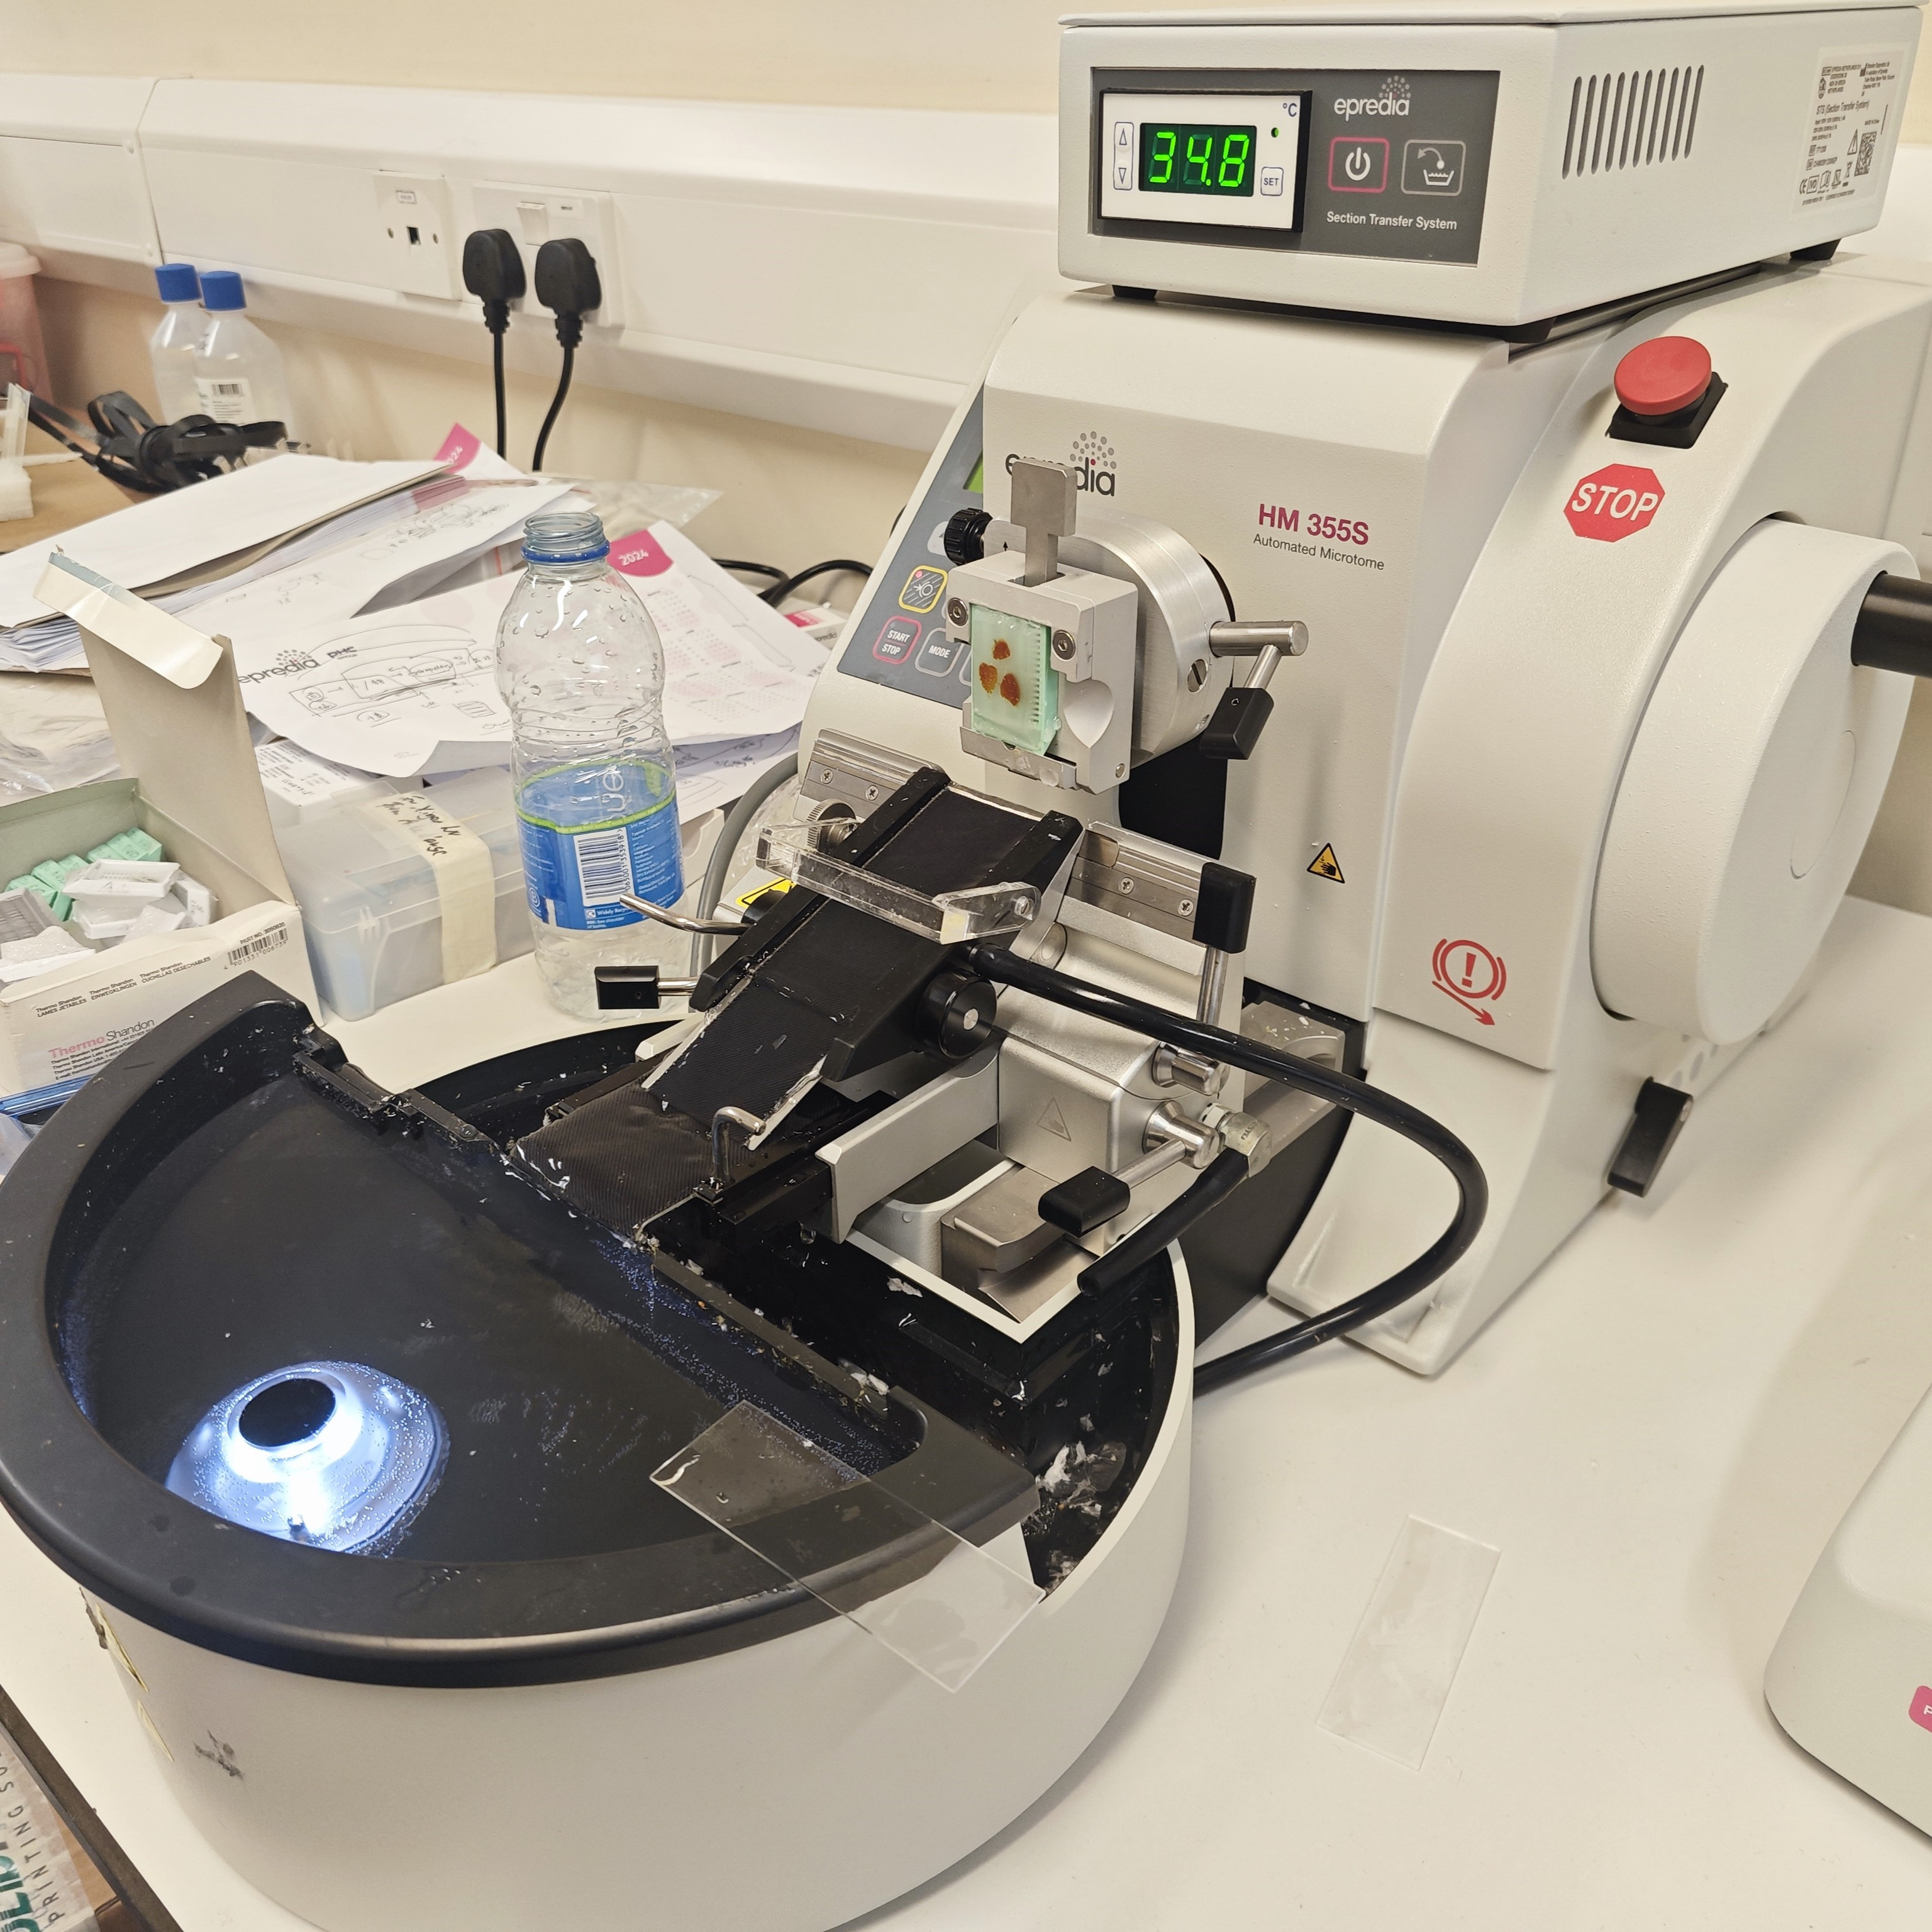
\includegraphics[width=\textwidth]{./fig/machine.jpg}
        \caption{切片机}
        \label{fig:machine}
    \end{minipage}
    \begin{minipage}{0.35\textwidth}
        \centering
        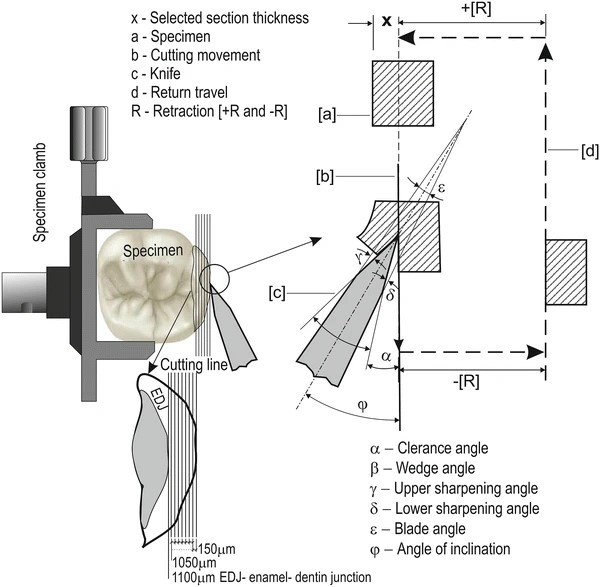
\includegraphics[width=\textwidth]{./fig/10266_2018_353_Fig1_HTML.jpg}
        \caption{切片机示意图}
        \label{fig:cutting_machine}
    \end{minipage}
\end{figure}
% https://link.springer.com/article/10.1007/s10266-018-0353-6



% 在切削过程中,从切角为8度开始(如\autoref{fig:machine}中的angle of inclination),每次增加0.5度,直到切角为12度。切片机在切片过程中保持给进速度为25,厚度为1。

在我们的实验中,我们使用切片机的参数如下:模式设置为连续,进给速度为5.0,修整值为25,速度为32,水流速度为7.5,水温约为36摄氏度,切割角度在8到12度之间。

用于切片的生物组织(示例)如\autoref{label:sample}所示

在切片完成之后,将切好的不同类型的组织切片放在载玻片上(如\autoref{fig:采集样本})所示,待其晾干后转移至VHX7000显微镜下,通过显微镜对每份样品进行拍照,获取到每份样品的电子图像数据(如\autoref{fig:显微镜})。

\begin{figure}[htbp]
    \centering
    \begin{minipage}{0.3\textwidth}
        \centering
        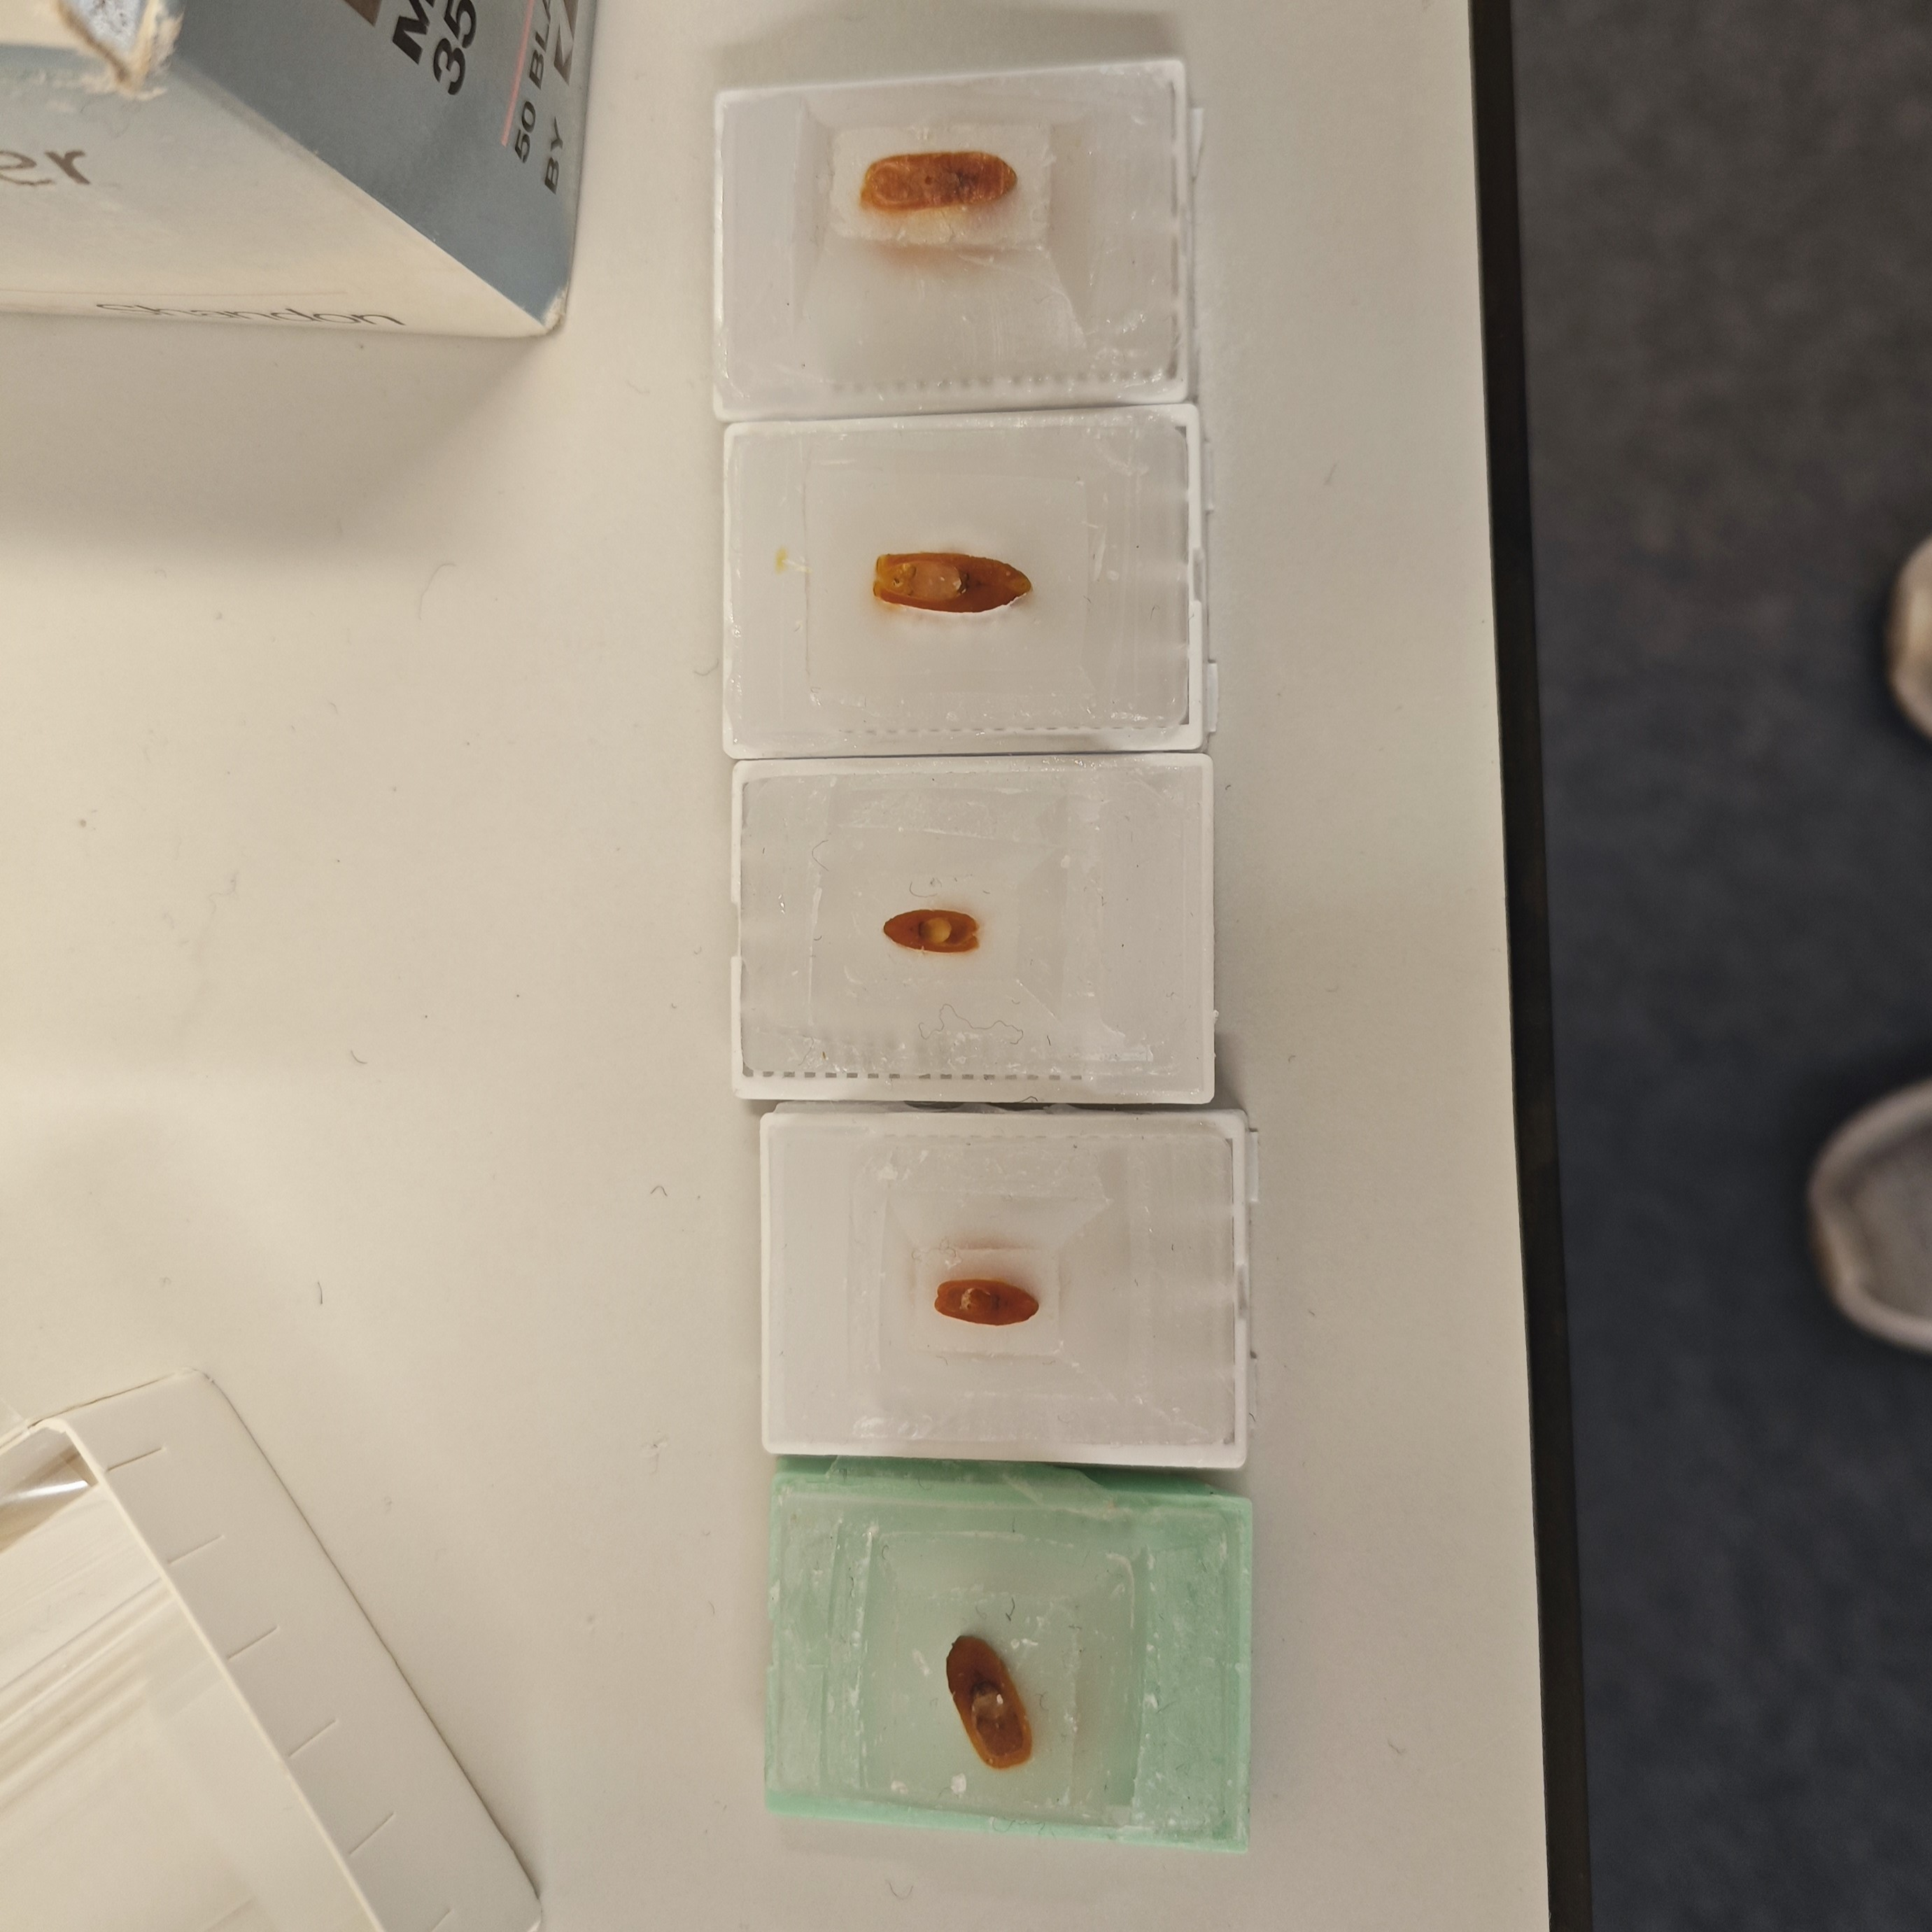
\includegraphics[width=\textwidth]{./fig/sample.jpg}
        \caption{生物组织切片}
        \label{label:sample}
    \end{minipage}
    \begin{minipage}{0.3\textwidth}
        \centering
        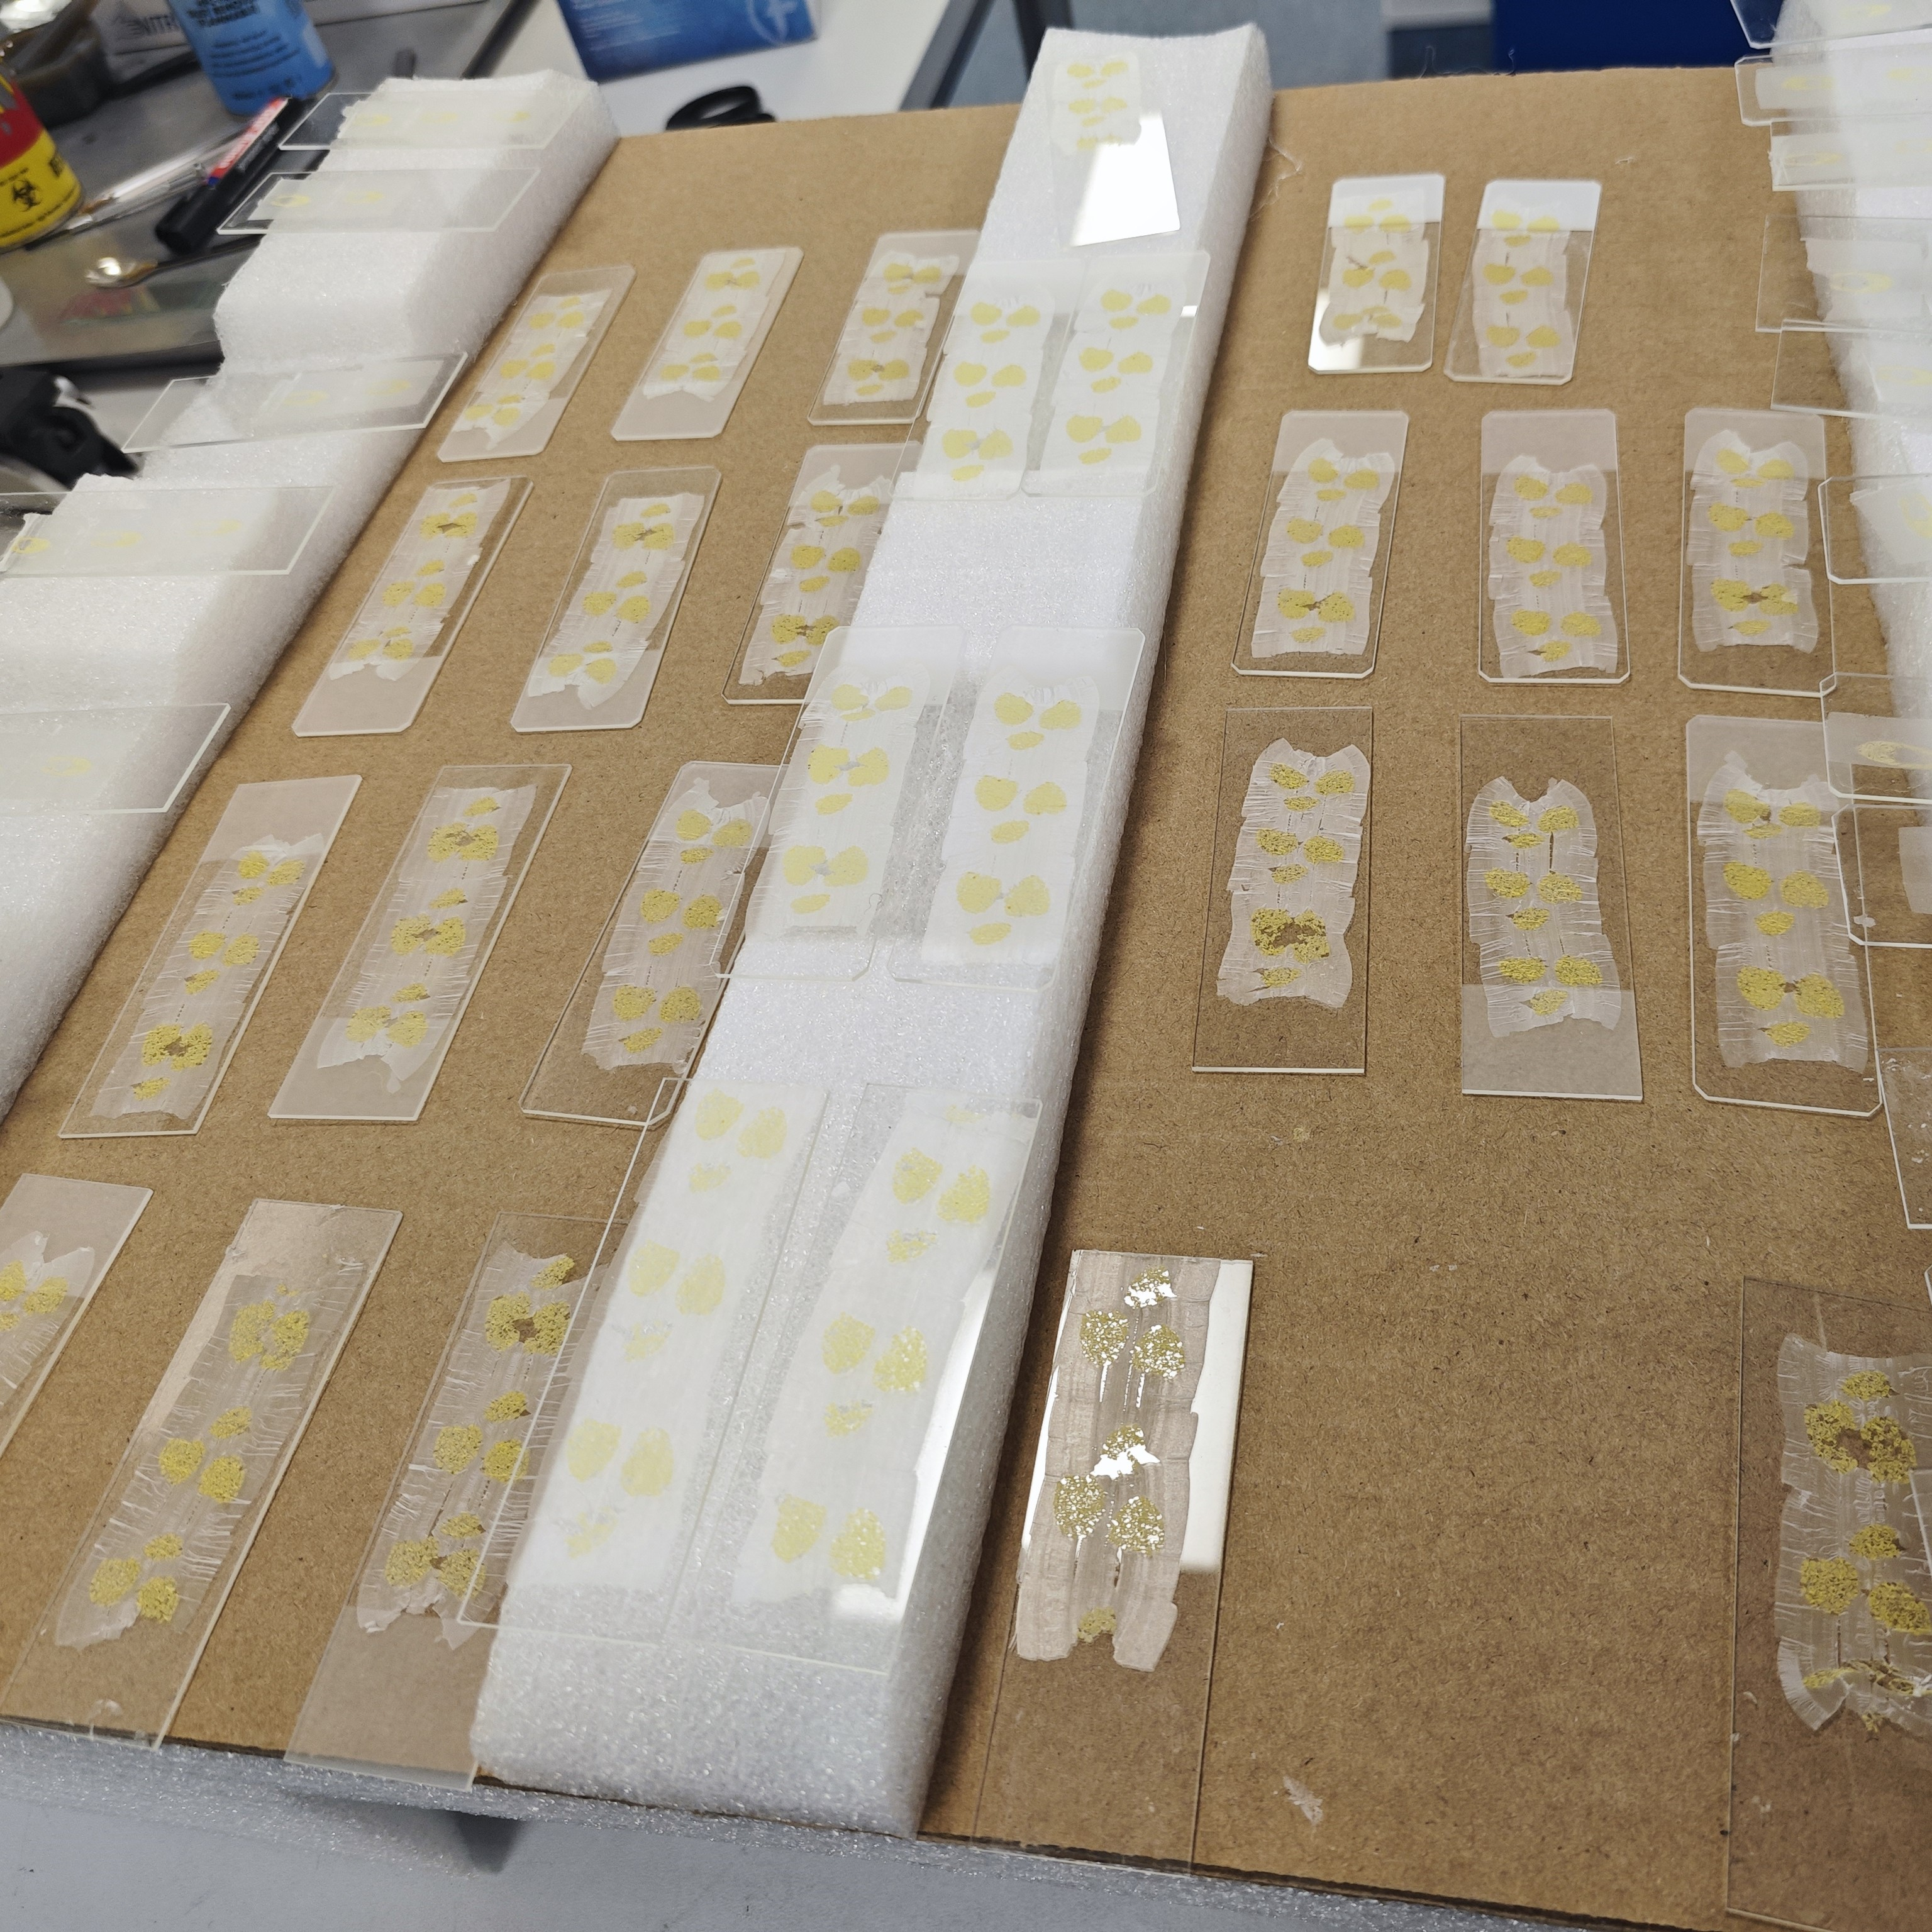
\includegraphics[width=\textwidth]{./fig/采集样本.jpg}
        \caption{采集样本}
        \label{fig:采集样本}
    \end{minipage}
    \begin{minipage}{0.35\textwidth}
        \centering
        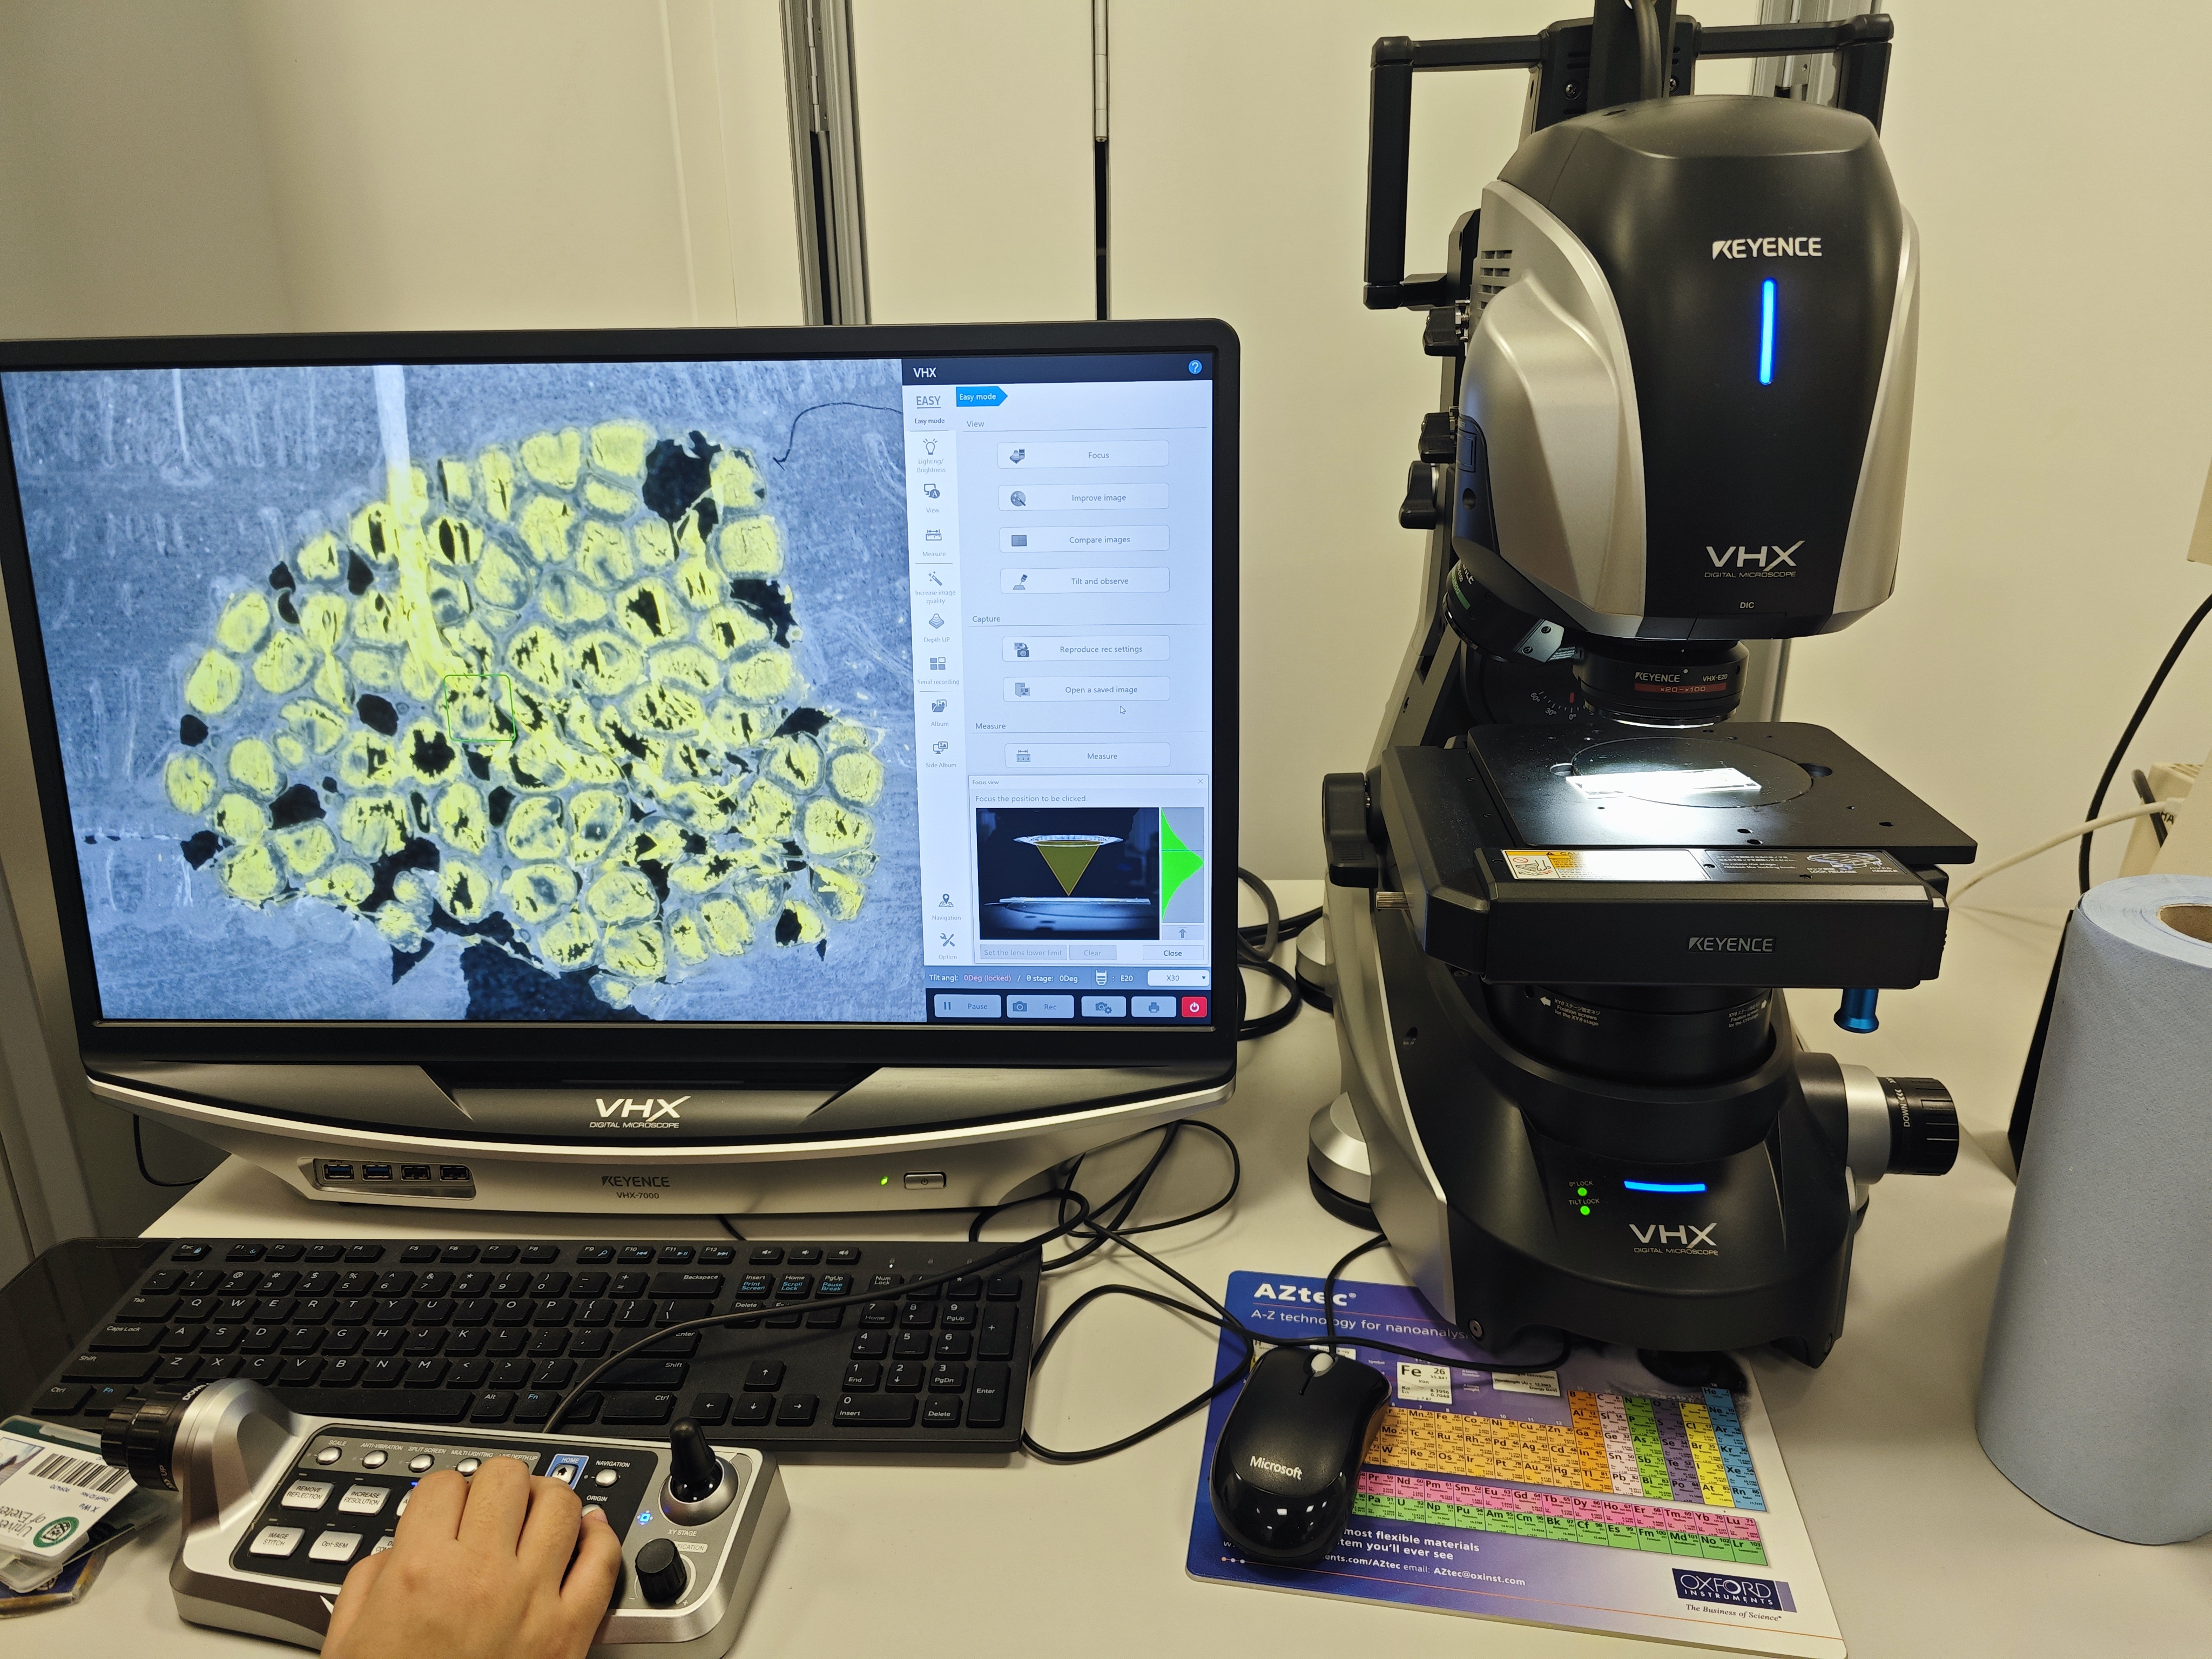
\includegraphics[width=\textwidth]{./fig/显微镜.jpg}
        \caption{显微镜}
        \label{fig:显微镜}
    \end{minipage}
\end{figure}

%图片需要后续更改为卵巢的

% 据此,一共得到几百张图片,每张图片的分辨率为2880*2160。样本示例如\autoref{fig:sample9.5}所示。

% \begin{figure}
%     \centering
%     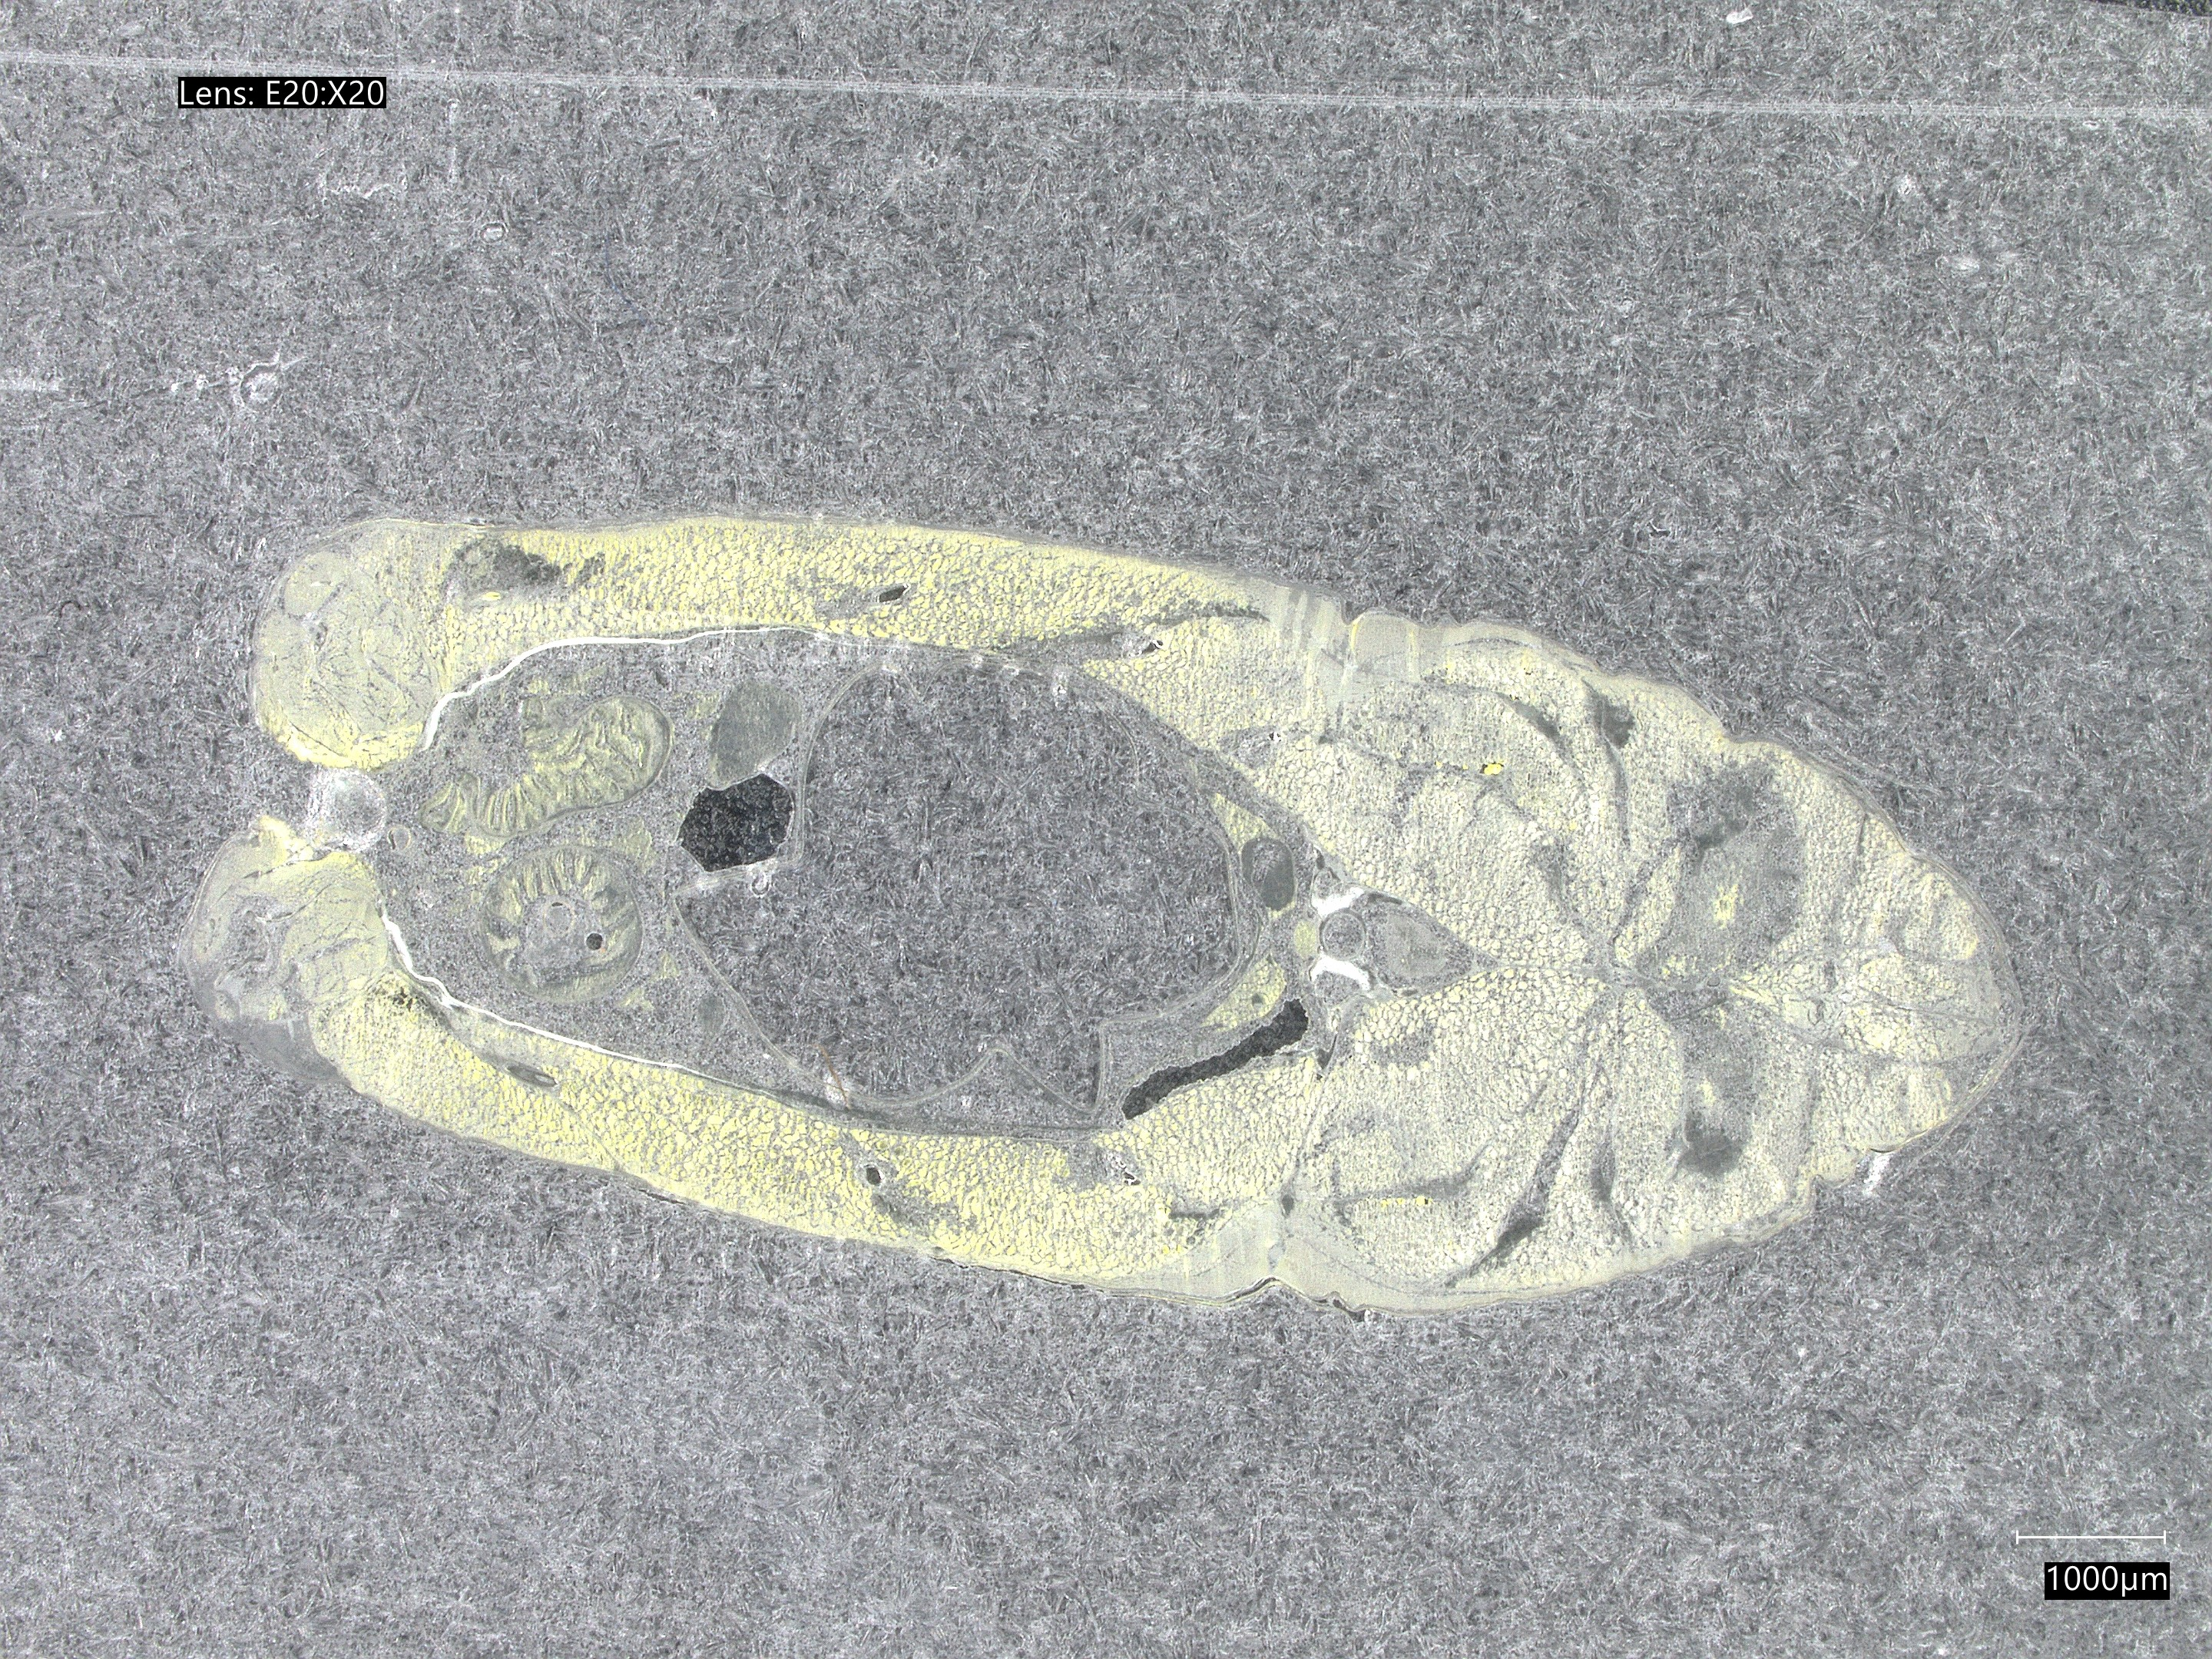
\includegraphics[width=0.8\textwidth]{./fig/sample9.5.jpg}
%     \caption{切角9.5度的样本}
%     \label{fig:sample9.5}
% \end{figure}


\subsection{标注数据}

对于这个实验,数据集是根据组织切片的质量进行标记的。总的来说,生物组织的质量被分为两个主要类别:正常和不良。对收集的数据进行进一步分析,发现了常见的缺陷 - 切片上存在垂直或水平的白色皱纹,这明显表明切片无法使用。鉴于这些缺陷的独特性质,它们被分类为两个额外的特定类别:\textbf{水平线}(见\autoref{fig:horizental_line})和\textbf{垂直线}(见\autoref{fig:vertical_line})。

\begin{figure}[H]
    \centering
    \begin{minipage}{0.33\textwidth}
        \centering
        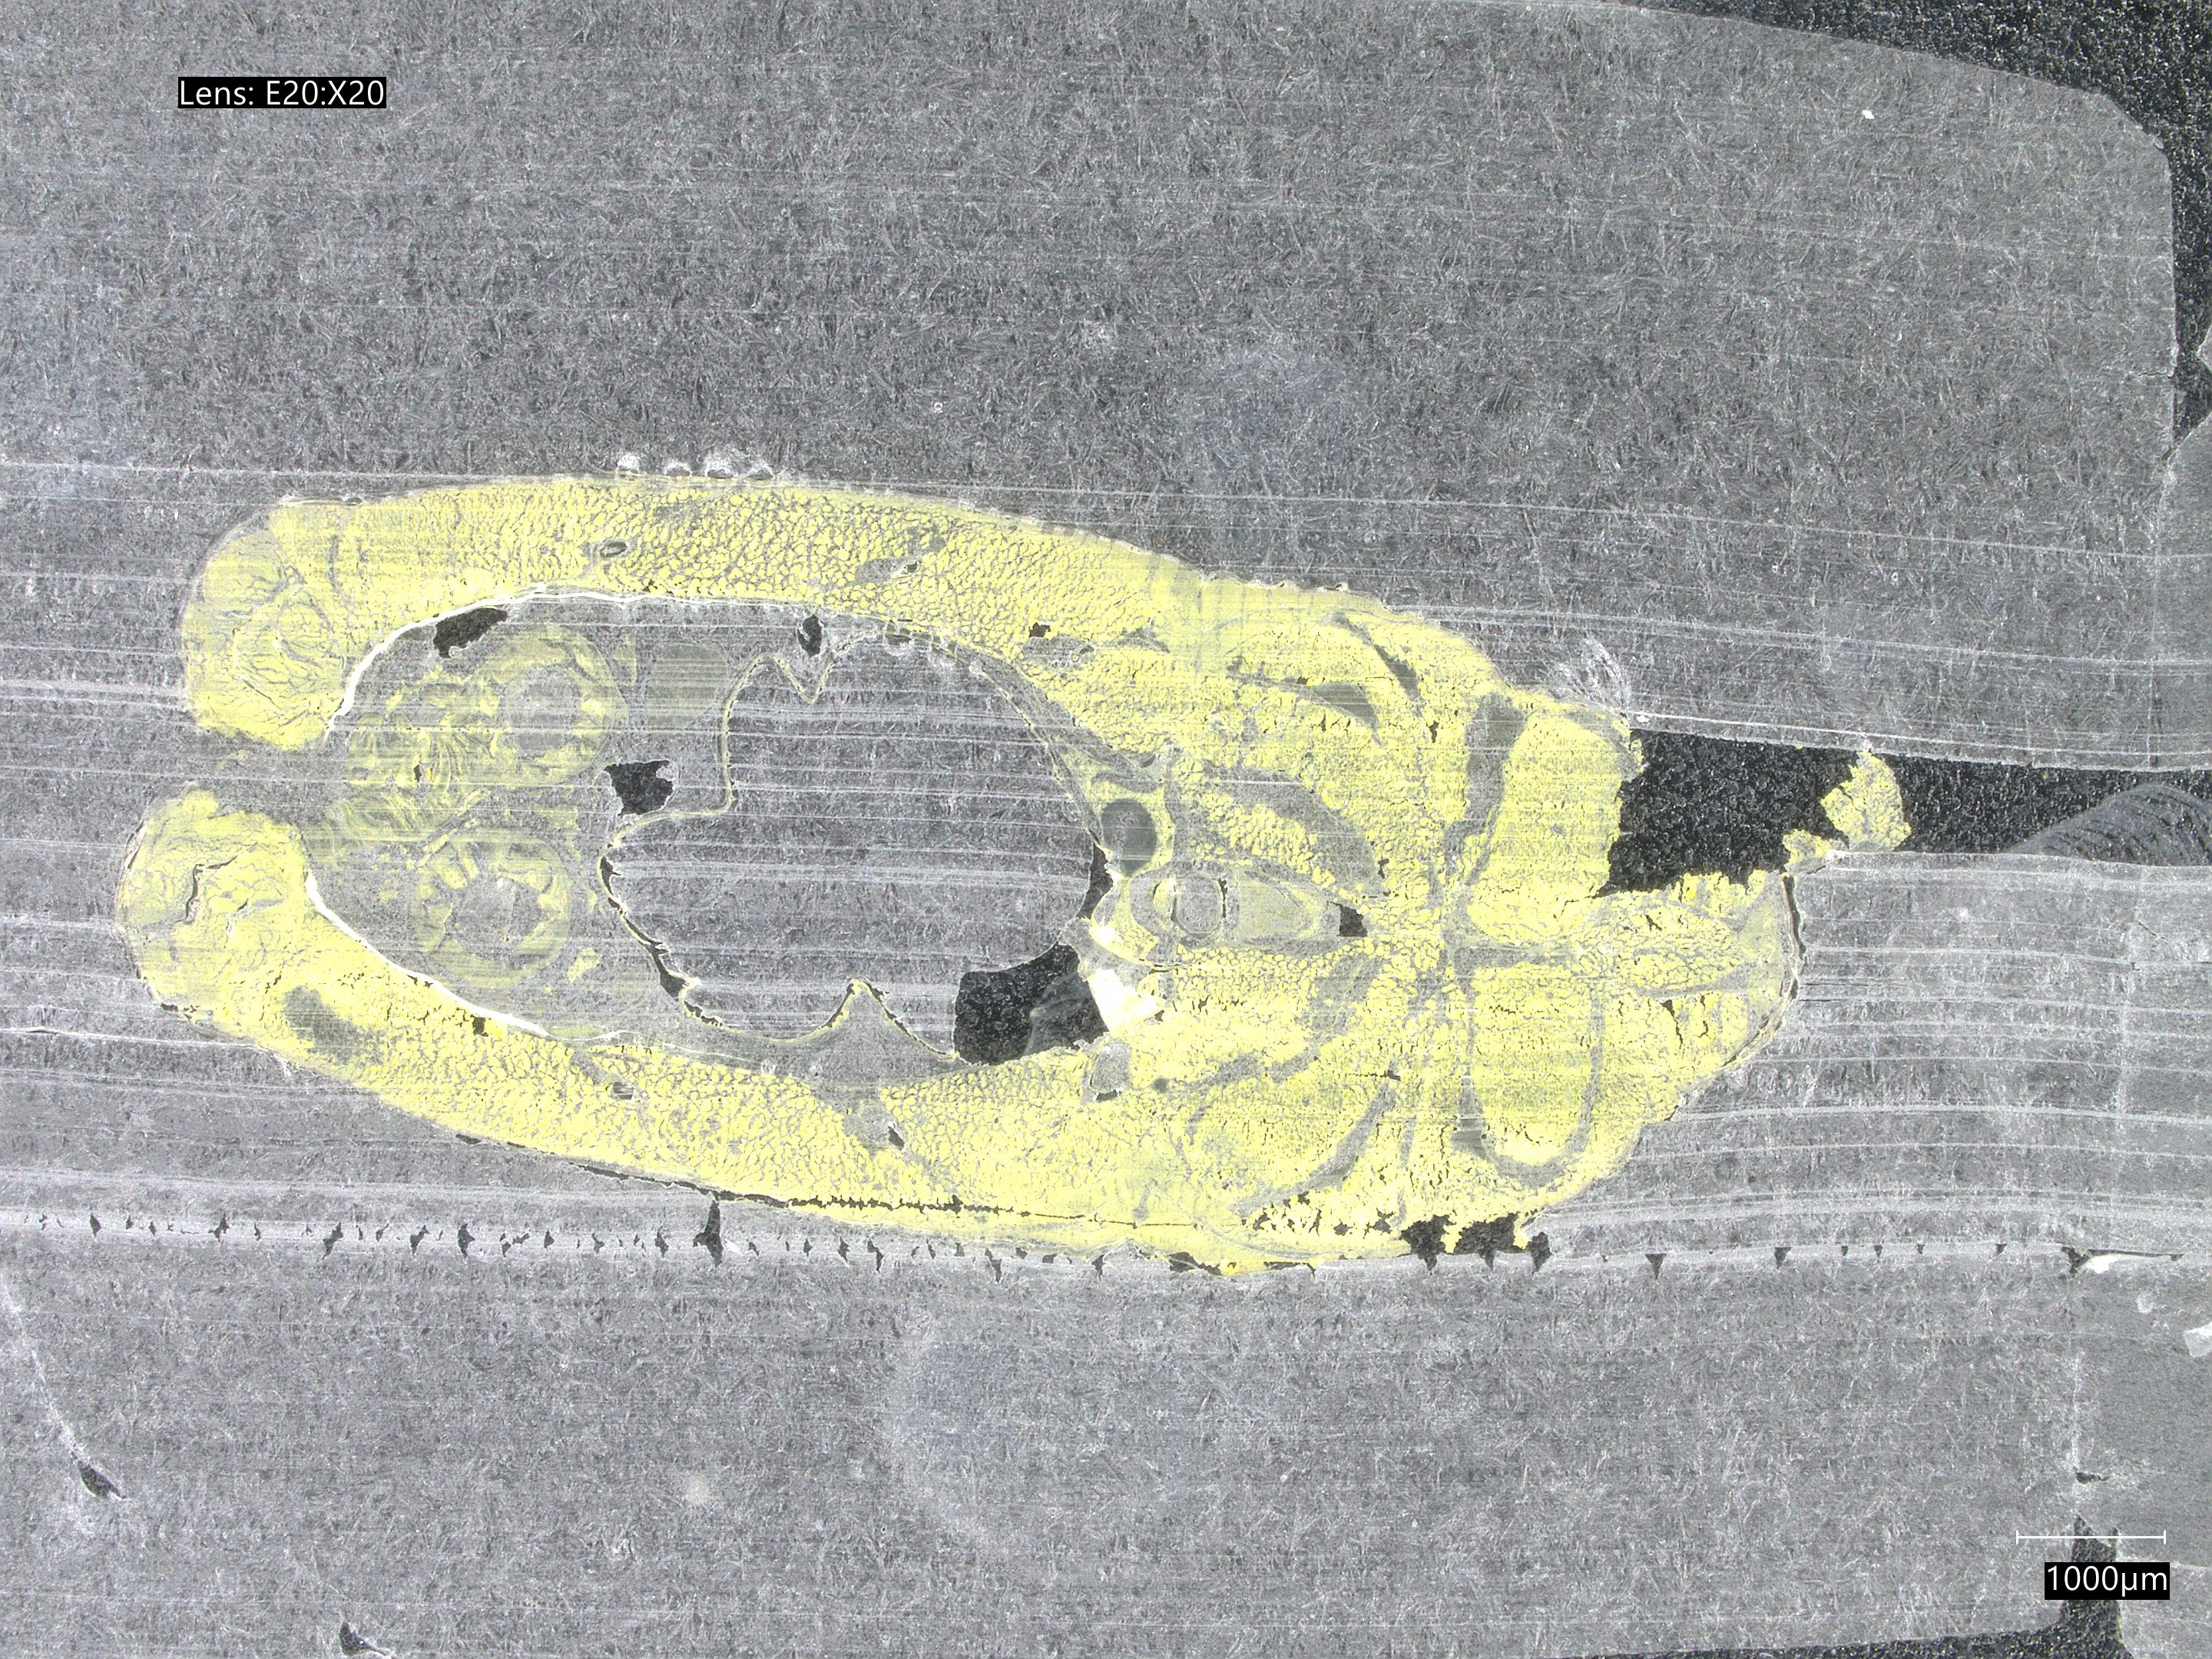
\includegraphics[width=\textwidth]{./fig/sample_1/horizental_line.jpg}
        \caption{horizental line}
        \label{fig:horizental_line}
    \end{minipage}
    \begin{minipage}{0.33\textwidth}
        \centering
        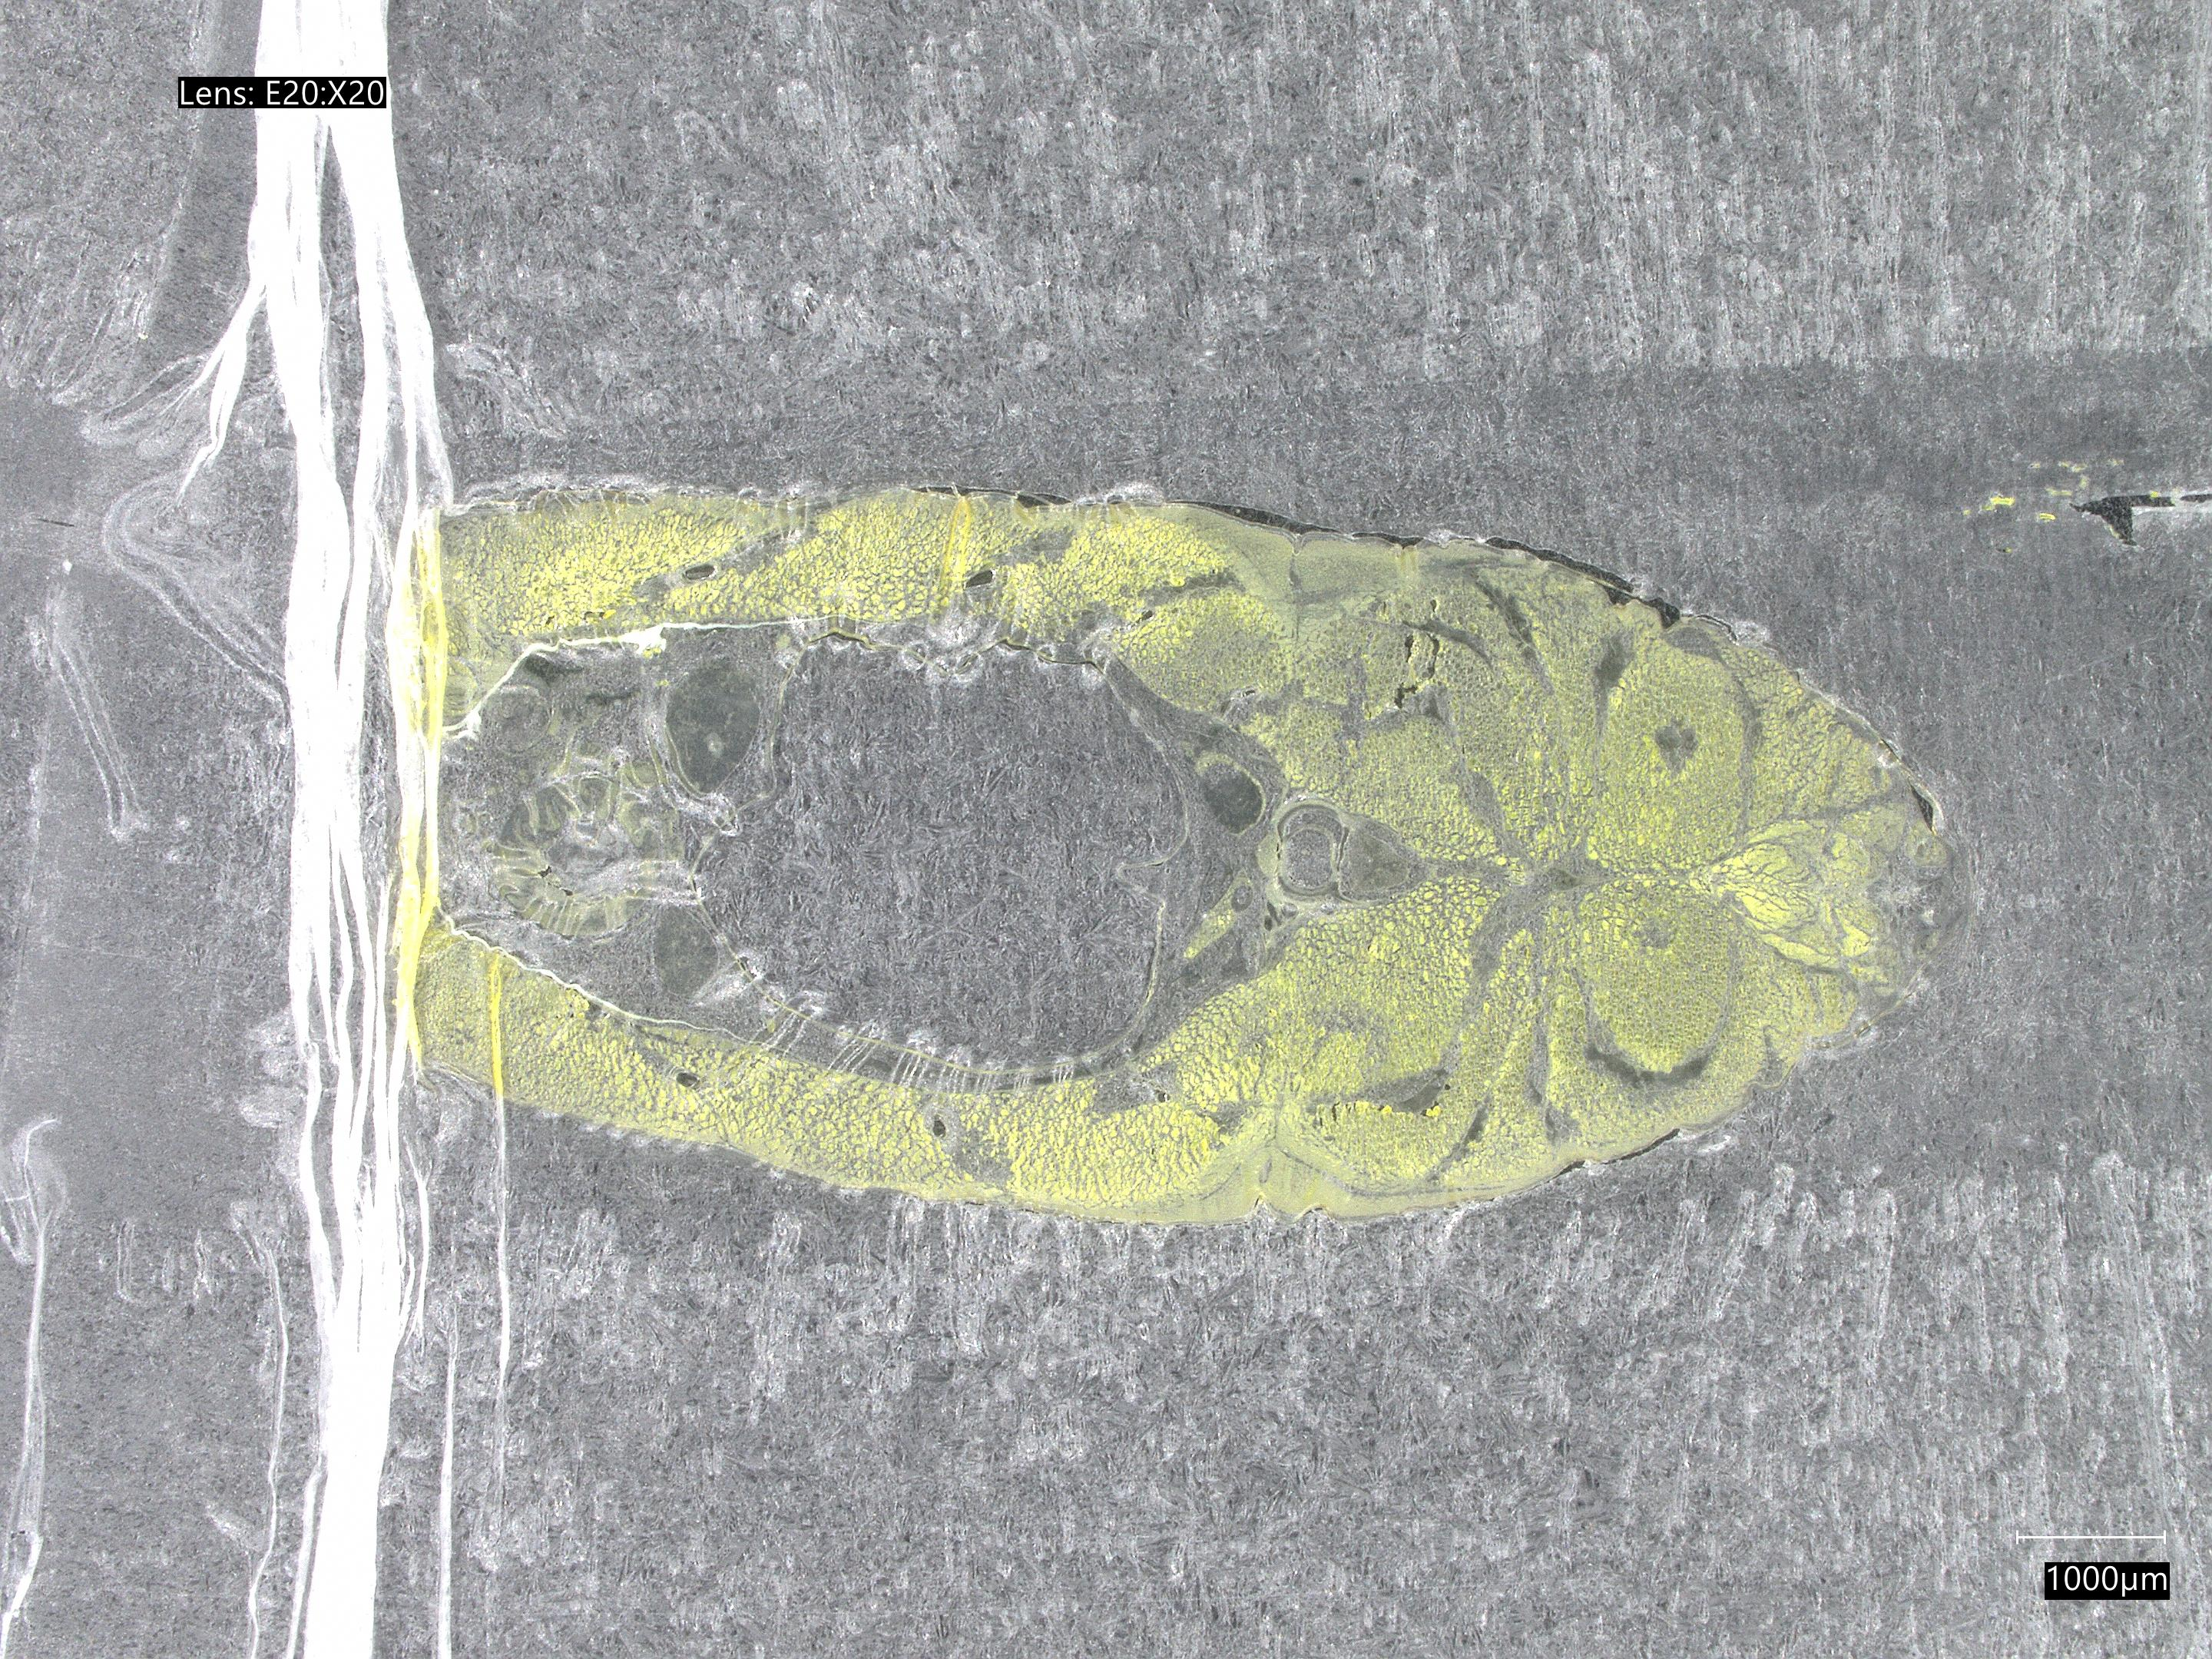
\includegraphics[width=\textwidth]{./fig/sample_1/vertical_line.jpg}
        \caption{vertical line}
        \label{fig:vertical_line}
    \end{minipage}
\end{figure}

此外,考虑到有一部分图片在采样时存在明显的旋转角度,这种情况下,我们也将其单独分为一类,称为slope(如图\autoref{fig:slope})。最后,对于剩下的图片,我们将其标注为other(如图\autoref{fig:other})。

\begin{figure}[H]
    \centering
    \begin{minipage}{0.32\textwidth}
        \centering
        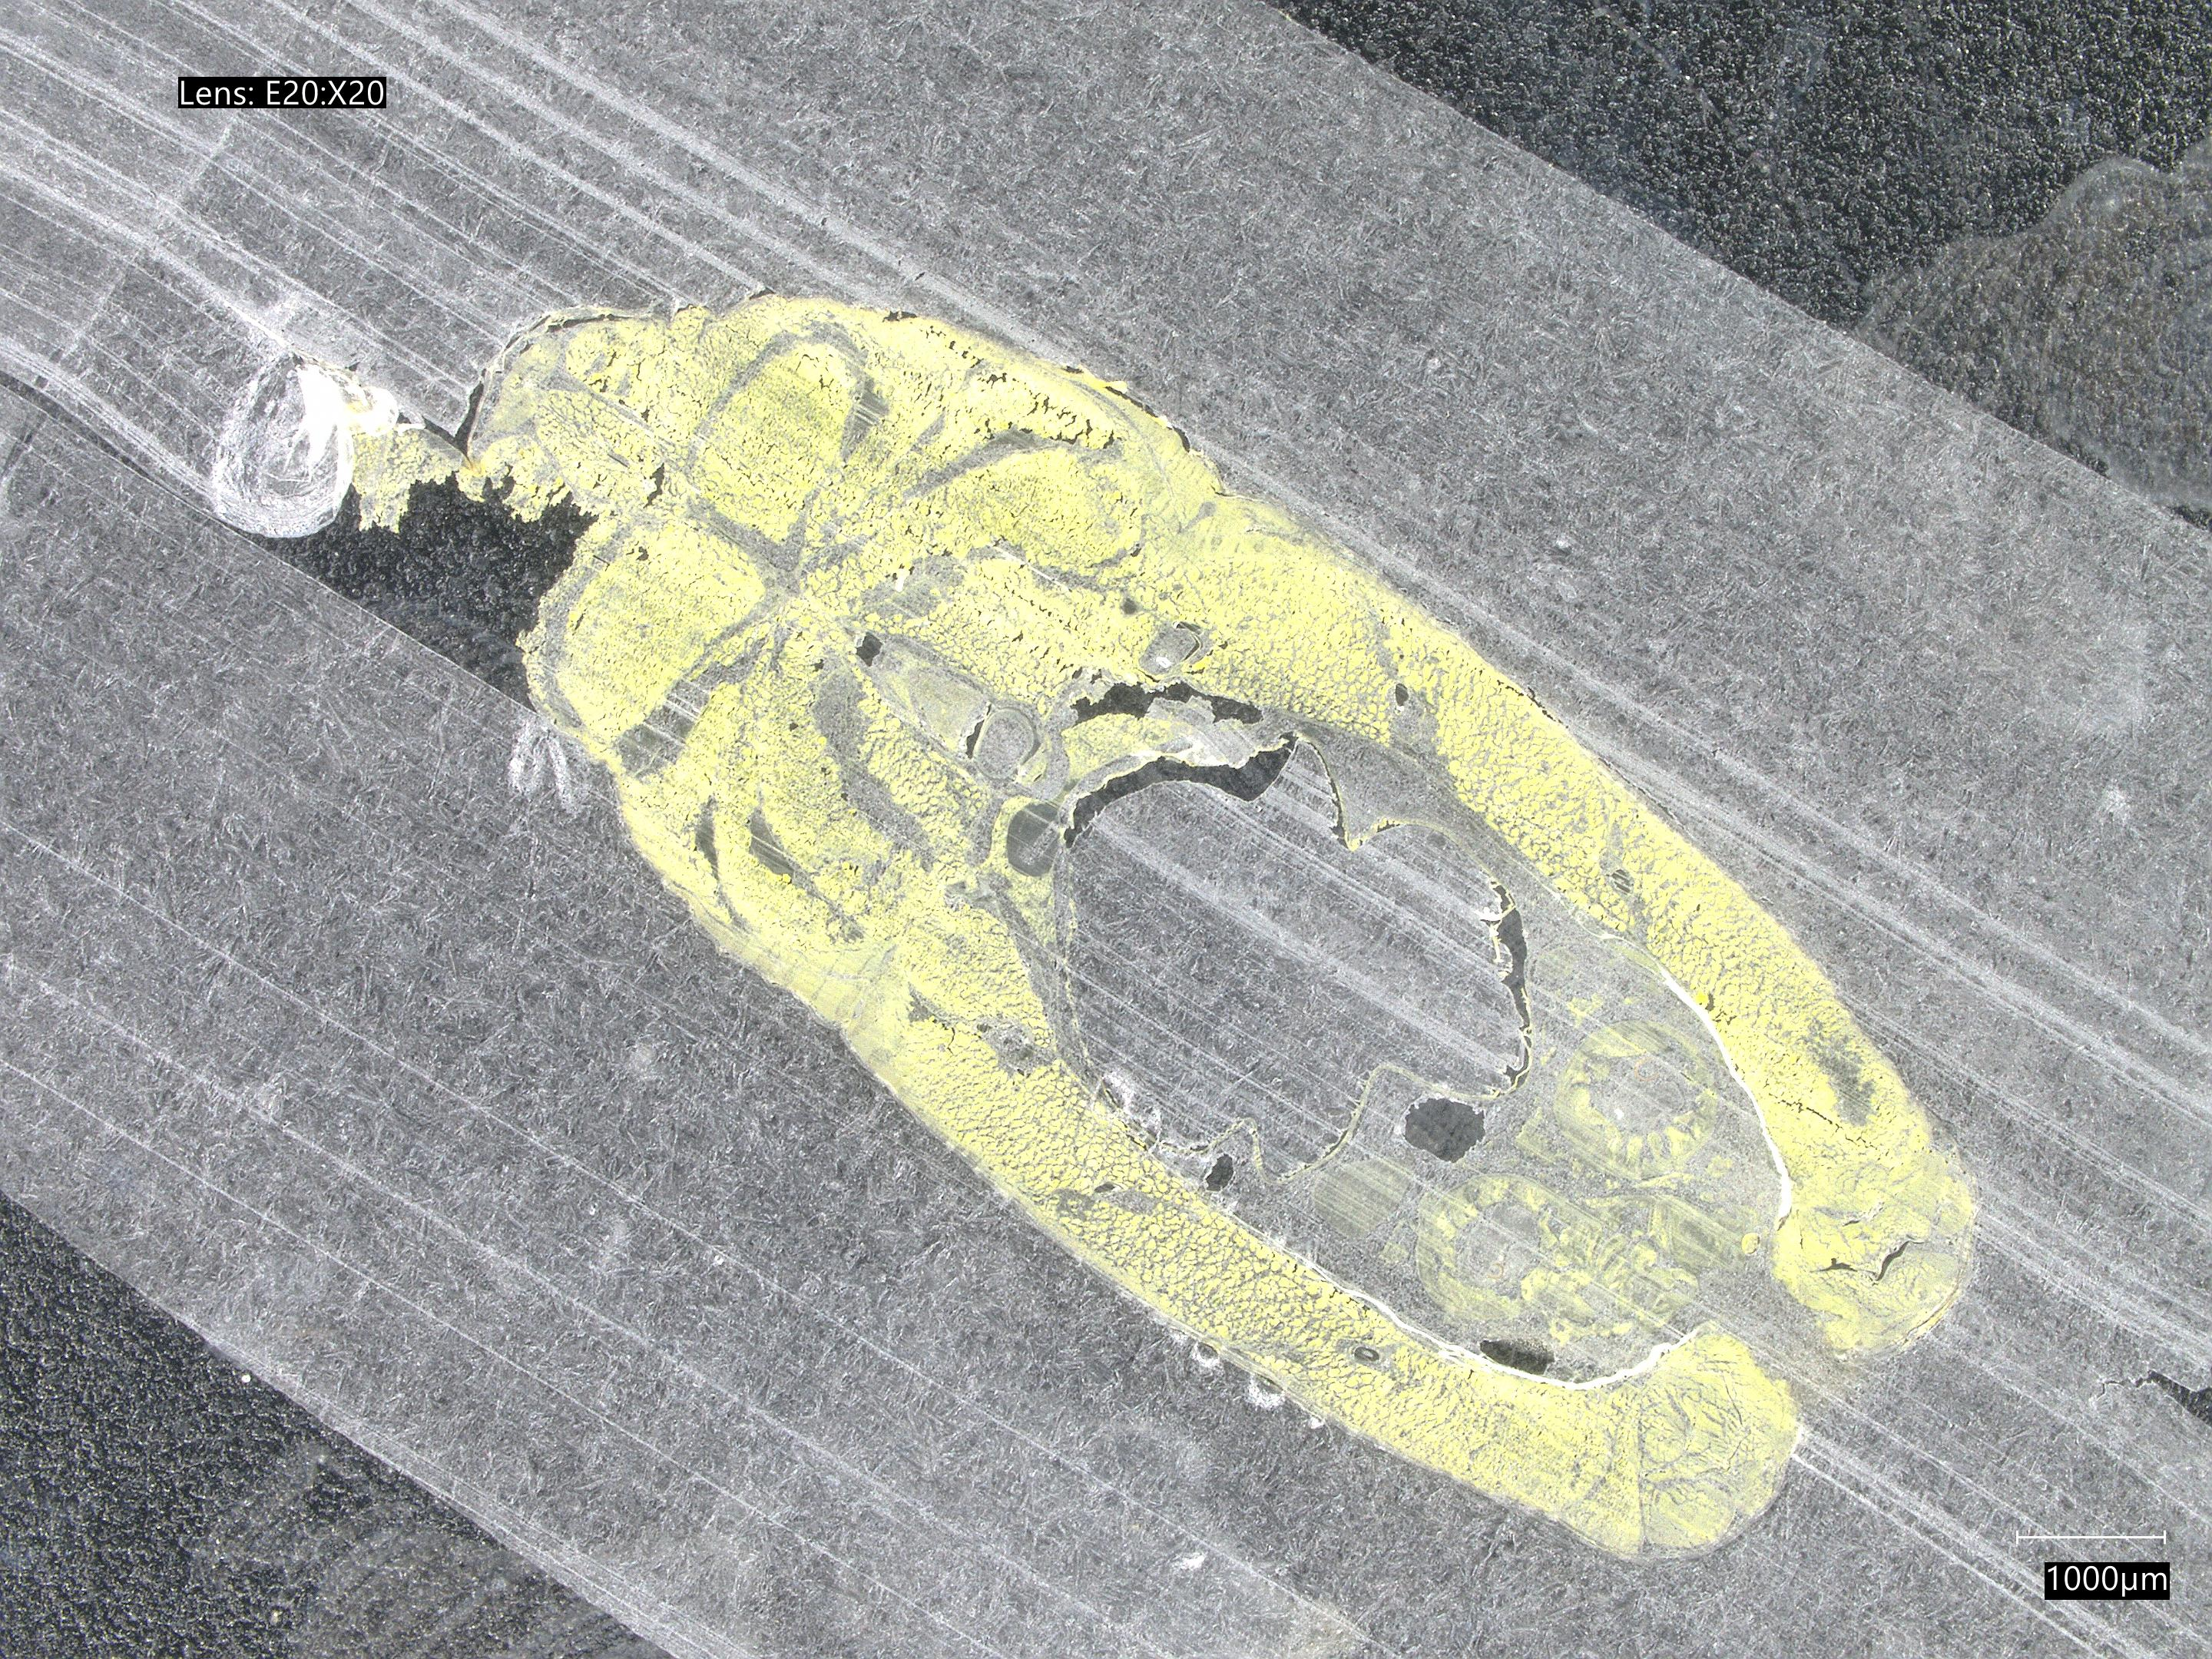
\includegraphics[width=\textwidth]{./fig/sample_1/slope.jpg}
        \caption{slope}
        \label{fig:slope}
    \end{minipage}
    \begin{minipage}{0.32\textwidth}
        \centering
        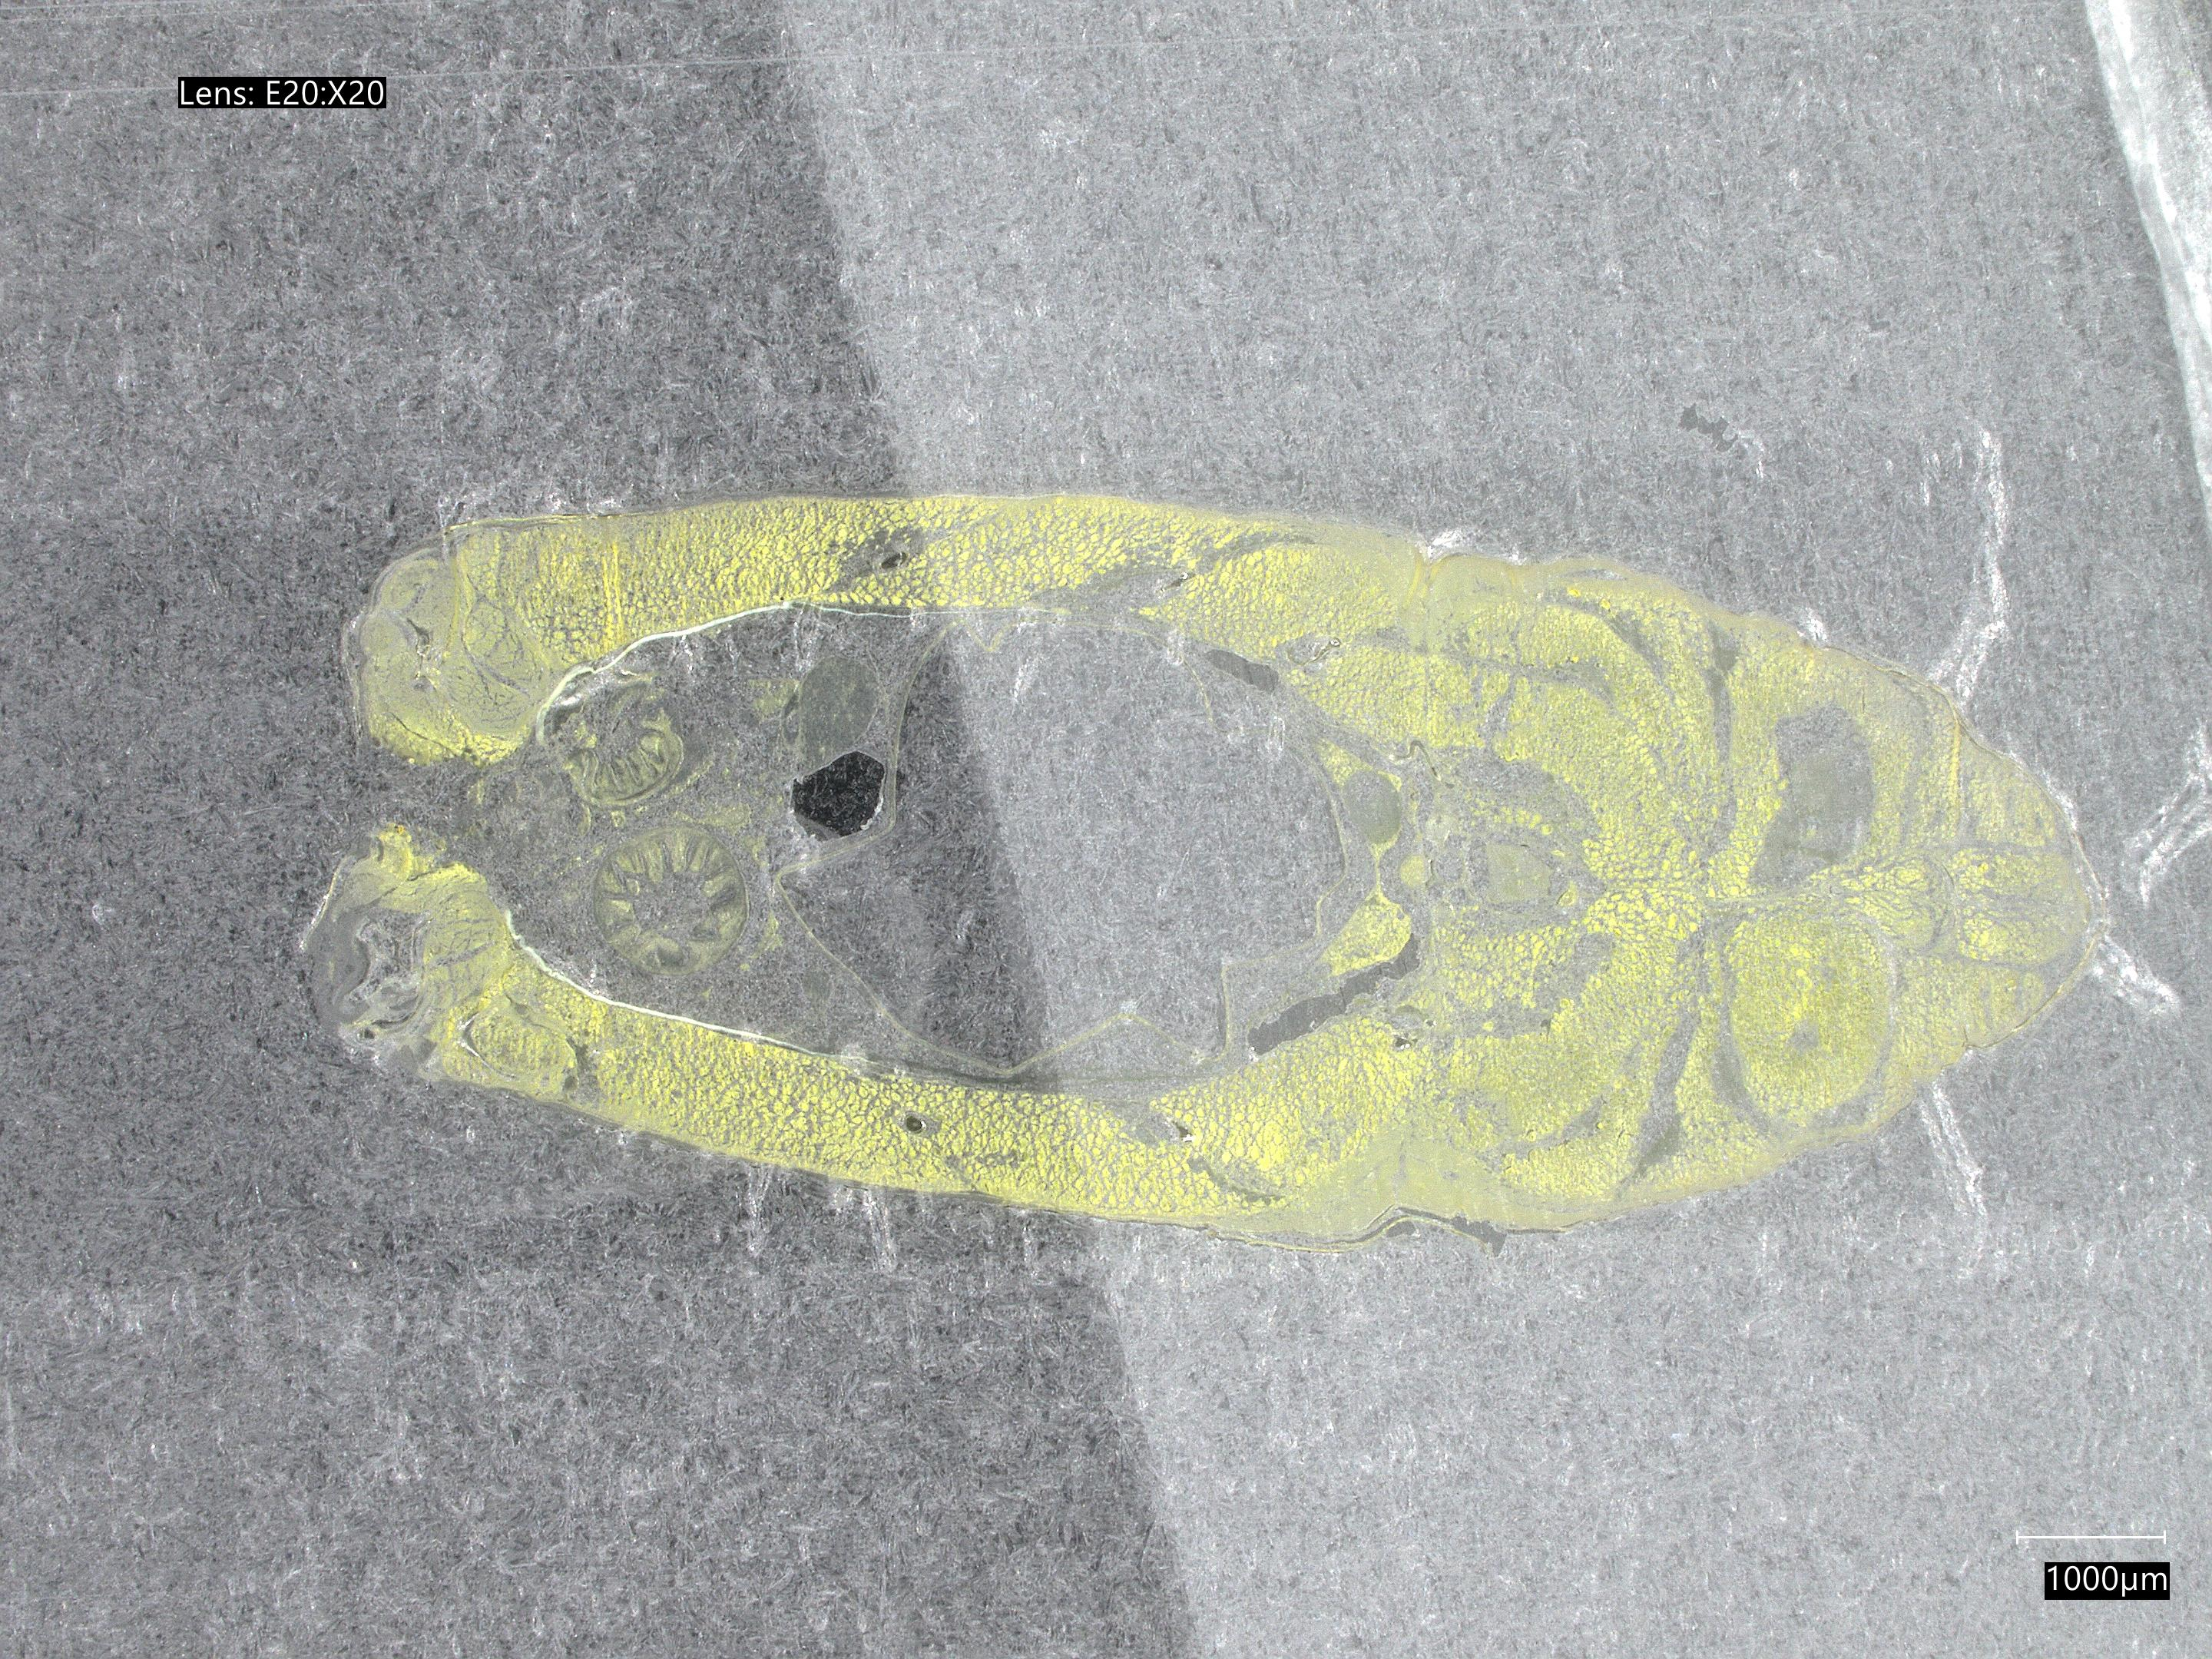
\includegraphics[width=\textwidth]{./fig/sample_1/other.jpg}
        \caption{other}
        \label{fig:other}
    \end{minipage}
    \begin{minipage}{0.32\textwidth}
        \centering
        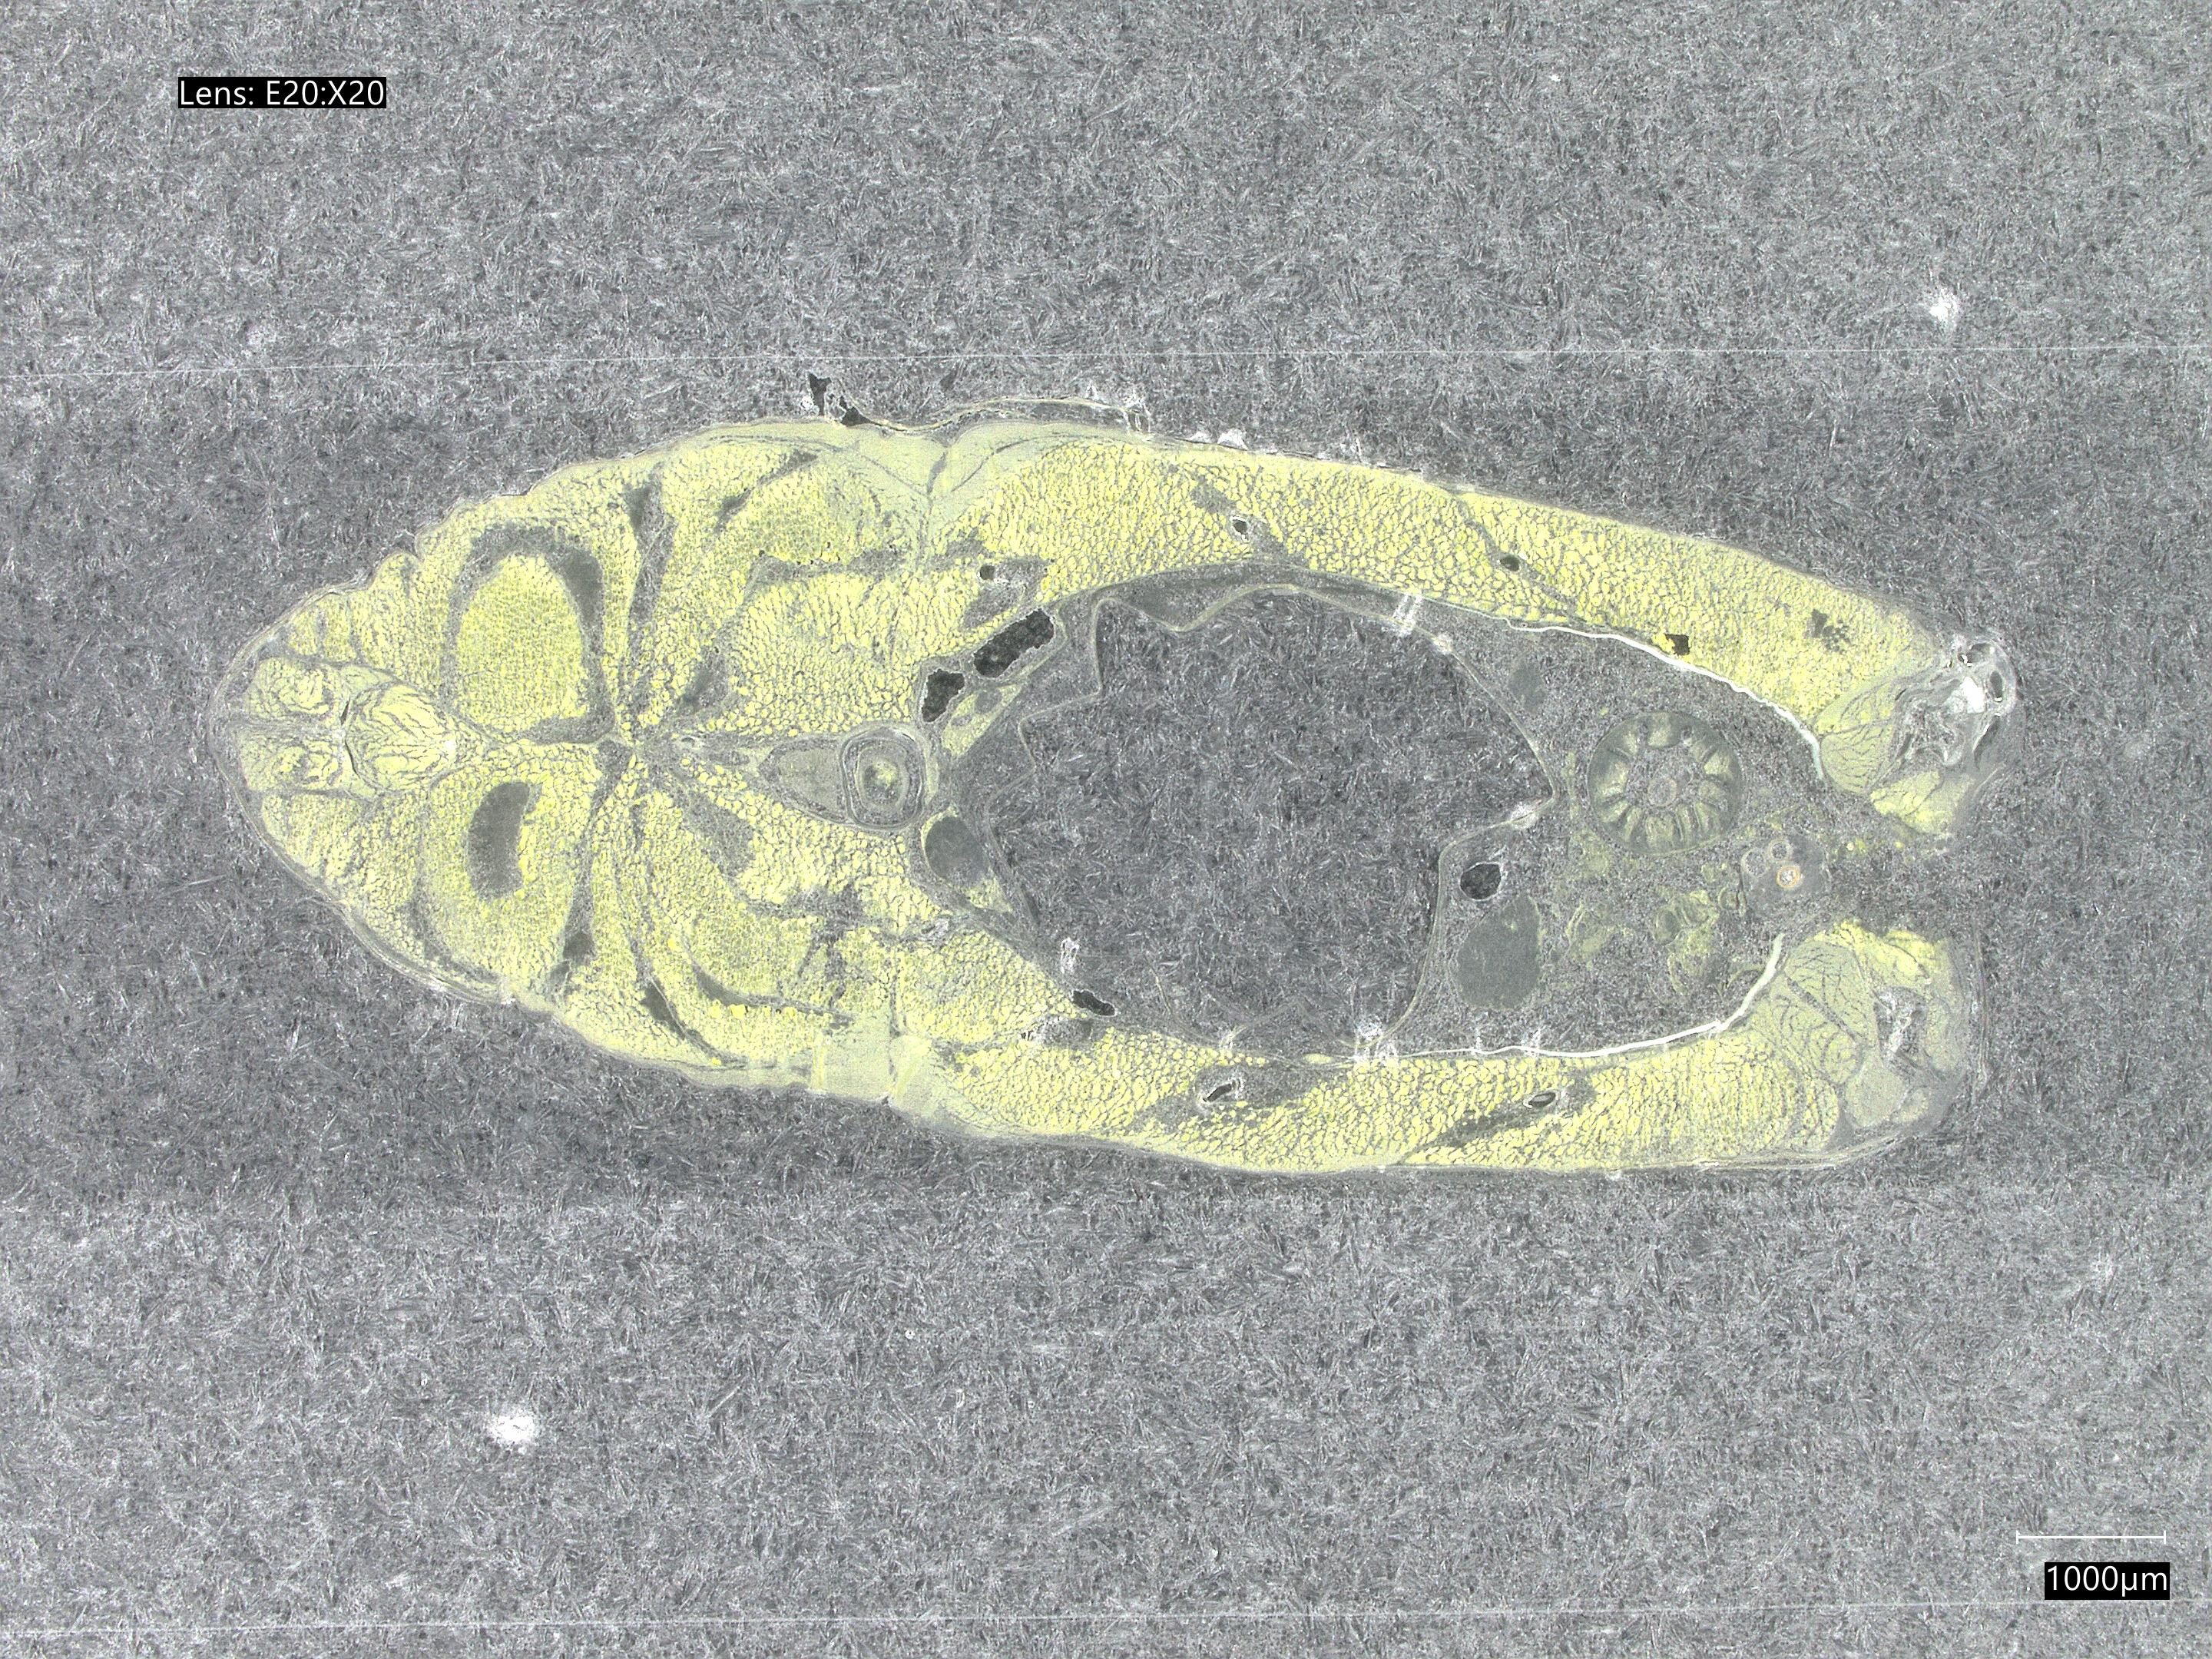
\includegraphics[width=\textwidth]{./fig/sample_1/normal.jpg}
        \caption{normal}
        \label{fig:normal}
    \end{minipage}
\end{figure}

正常的符合观察要求的切片如\autoref{fig:normal}所示。

对于每一张图片,我们需要将其标注为以上五个类别中的一个。这将作为我们的数据集,用于训练模型。


\FloatBarrier

\subsection{模型1:原始图像+简单的cnn网络}

对于一个全新的数据集,在不确定图像复杂度对应的何种模型之前,
首先尝试一个简单的典型cnn网络(架构如下),以了解数据集的特点和图像复杂度。

\begin{table}[H]
\centering
\caption{Configuration of the simple CNN model}
\begin{tabular}{ccccc}
    \toprule
    \textbf{Layer Type} & \textbf{Configuration 1a} & \textbf{Configuration 1b} & \textbf{Configuration 1c} \\
    \midrule
    Input Layer & - & - & - \\
    Conv Layer 1 & Conv3-32 (relu) & Conv3-16 (relu) & Conv3-32 (relu) \\
    Pooling Layer 1 & MaxPooling & MaxPooling& MaxPooling \\
    Conv Layer 2 & Conv3-32 (relu) & Conv3-32 (relu) & Conv3-32 (relu) \\
    Pooling Layer 2 & MaxPooling & MaxPooling& MaxPooling \\
    Conv Layer 3 & Conv3-32 (relu) & Conv3-64 (relu) & Conv3-32 (relu) \\
    Pooling Layer 3 & MaxPooling & MaxPooling& MaxPooling \\
    Flattening Layer & Flatten() & Flatten() & Flatten() \\
    FC(Full connect) & Dense(128, relu) & Dense(128, relu) & Dense(256, relu) \\
    Output Layer & - & - & - \\
    \bottomrule
\end{tabular}
\label{tab:cnn_simple_configuration}
\end{table}

\autoref{tab:cnn_simple_configuration}显示的三个初始模型,分别为a,b,c。这三个模型的区别在于卷积层的数量和大小,全连接层的大小。a和b相比修改了卷积层的神经元数量,c相比a修改了全连接层的神经元数量。

在数据的预处理部分,先将数据集分为训练集和测试集,其中训练集占80\%,测试集占20\%。

在输入层,这里将图像的长宽缩小一倍(即输入大小从2880*2160变为1440*1080)并归一化数据。

在训练过程中,我们使用了Adam优化器,交叉熵损失函数,使用早停。

下面图组展示了模型1a,1b,1c的准确度和损失随着训练次数的变化。

\begin{figure}[H]
    \centering
    \begin{minipage}{0.49\textwidth}
        \centering
        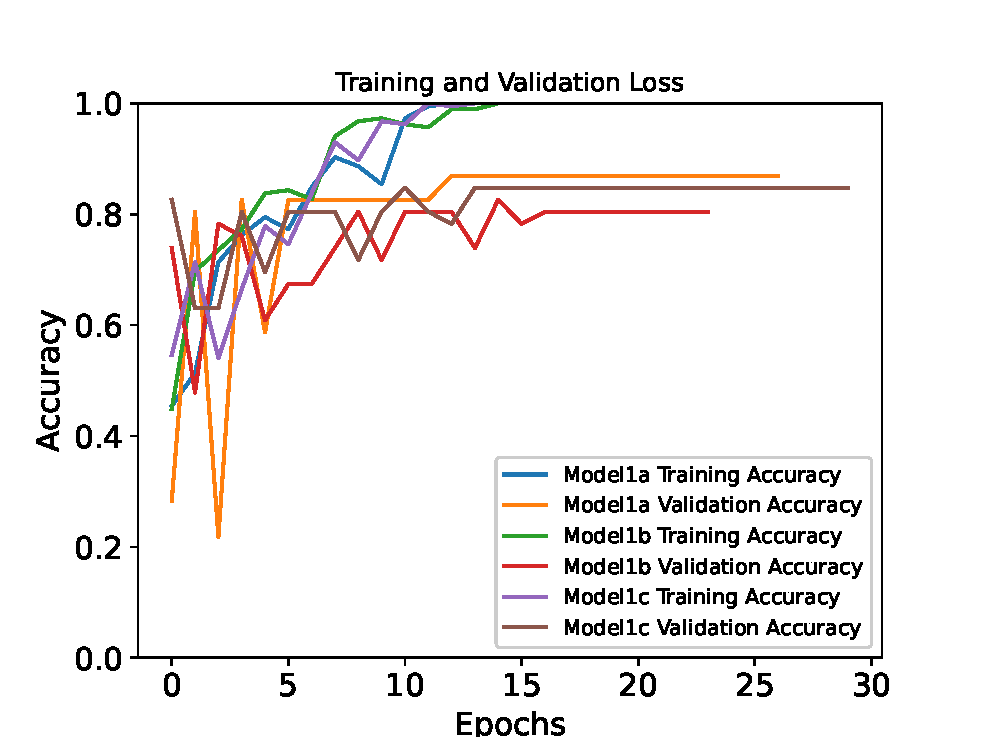
\includegraphics[width=\textwidth]{./fig/model1/accuracy11.eps}
        \caption{Model 1 accuracy}
        \label{fig:model11_acc}
    \end{minipage}
    \begin{minipage}{0.49\textwidth}
        \centering
        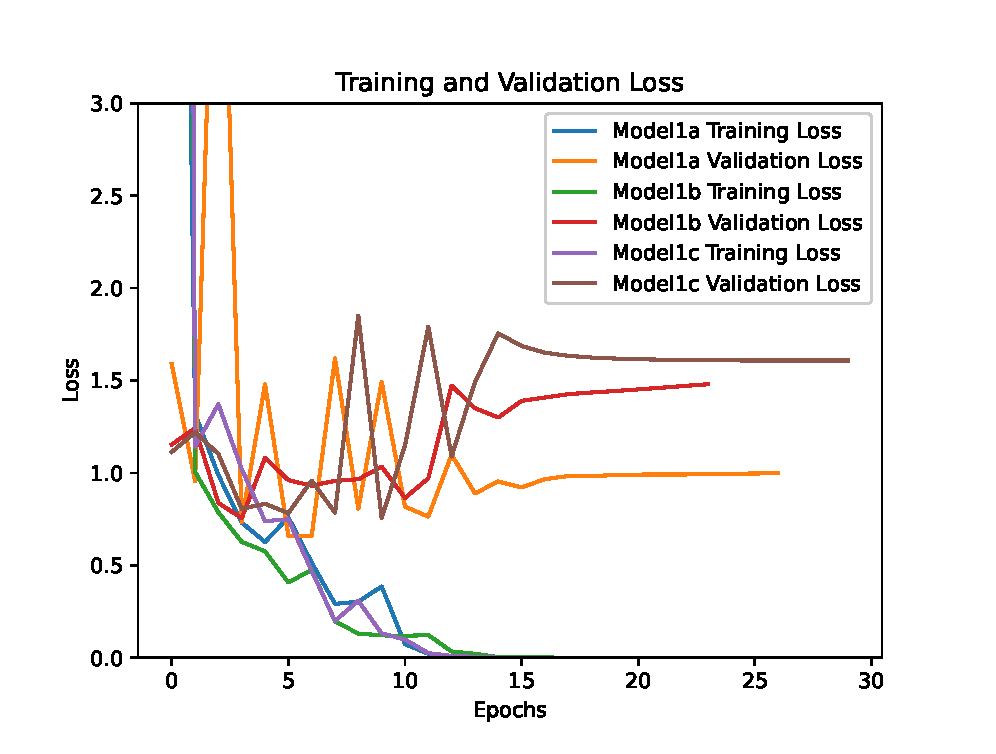
\includegraphics[width=\textwidth]{./fig/model1/loss11.eps}
        \caption{Model 1 loss}
        \label{fig:model11_loss}
    \end{minipage}
\end{figure}


在图中,观察到模型1a、1b和1c在不同训练周期(Epochs)的准确度与损失的变化情况。模型1a、1b和1c的训练准确度随着时间逐步提高,趋向于稳定,而训练损失则呈下降趋势,接近于零,这表明模型在学习训练数据方面表现得相对良好。然而,对于验证集,三个模型的准确度似乎在约80\%到85\%的区间内稳定,而验证损失在某些情况下较高,特别是模型1a的验证损失在后期趋近于2.5,表现出较大波动。这表明存在一定程度的过拟合,即模型在未见过的数据上的表现不如在训练集上。特别值得注意的是,模型1c相对于其他模型而言,在验证损失方面表现最佳,这可能意味着其结构或参数调整对于泛化能力的提升更为有效。

在这里过拟合的原因推测可能是模型的复杂度不够,数据集的复杂度过高,模型无法很好的提取特征。这些结果指出虽然模型在训练集上能够实现高准确度和低损失,但在验证集上的泛化能力还有待提高。

因此,我们考虑通过对图像的预处理,人为辅助计算机进行特征提取,以提高模型的准确性。
%具体的测试集测试在第五章

\FloatBarrier


\subsection{改进:图片预处理}

在模型表现能力欠佳的情况下,我们考虑是否是图像过于复杂导致模型难以提取出显著特征。因此我们考虑对图像进行预处理,以突出图像中我们希望让计算机识别的特征,并且在一定程度上去除图像的无关特征和噪声,以提高后续的深度学习模型的准确性。


在这里采用边缘检测,阈值分割两种方法对图像进行预处理。


\subsubsection{边缘检测}

正如在3.1.1中所提到的,边缘检测的原理是通过检测像素点的灰度值的变化(梯度)来确定图像中的边缘。

在进行边缘检测之前,还需要进行一步前处理-高斯模糊。这么做的原因是,高斯模糊可以减少图像中的噪声,平滑图像的梯度,减小识别假边缘的几率,使得边缘检测更加准确。\cite{4.3}在高斯模糊核的选择上,选择高斯核分别为21,41,61,81(图像宽度的1\%,2\%,3\%,4\%)。
高斯模糊后的图像如下所示。为了方便更直观的展示高斯模糊核对边缘检测的影响,这里采用sobel算子计算经过高斯模糊后的边缘并增加50的亮度。

\begin{figure}
    \centering
    \begin{minipage}{0.24\textwidth}
        \centering
        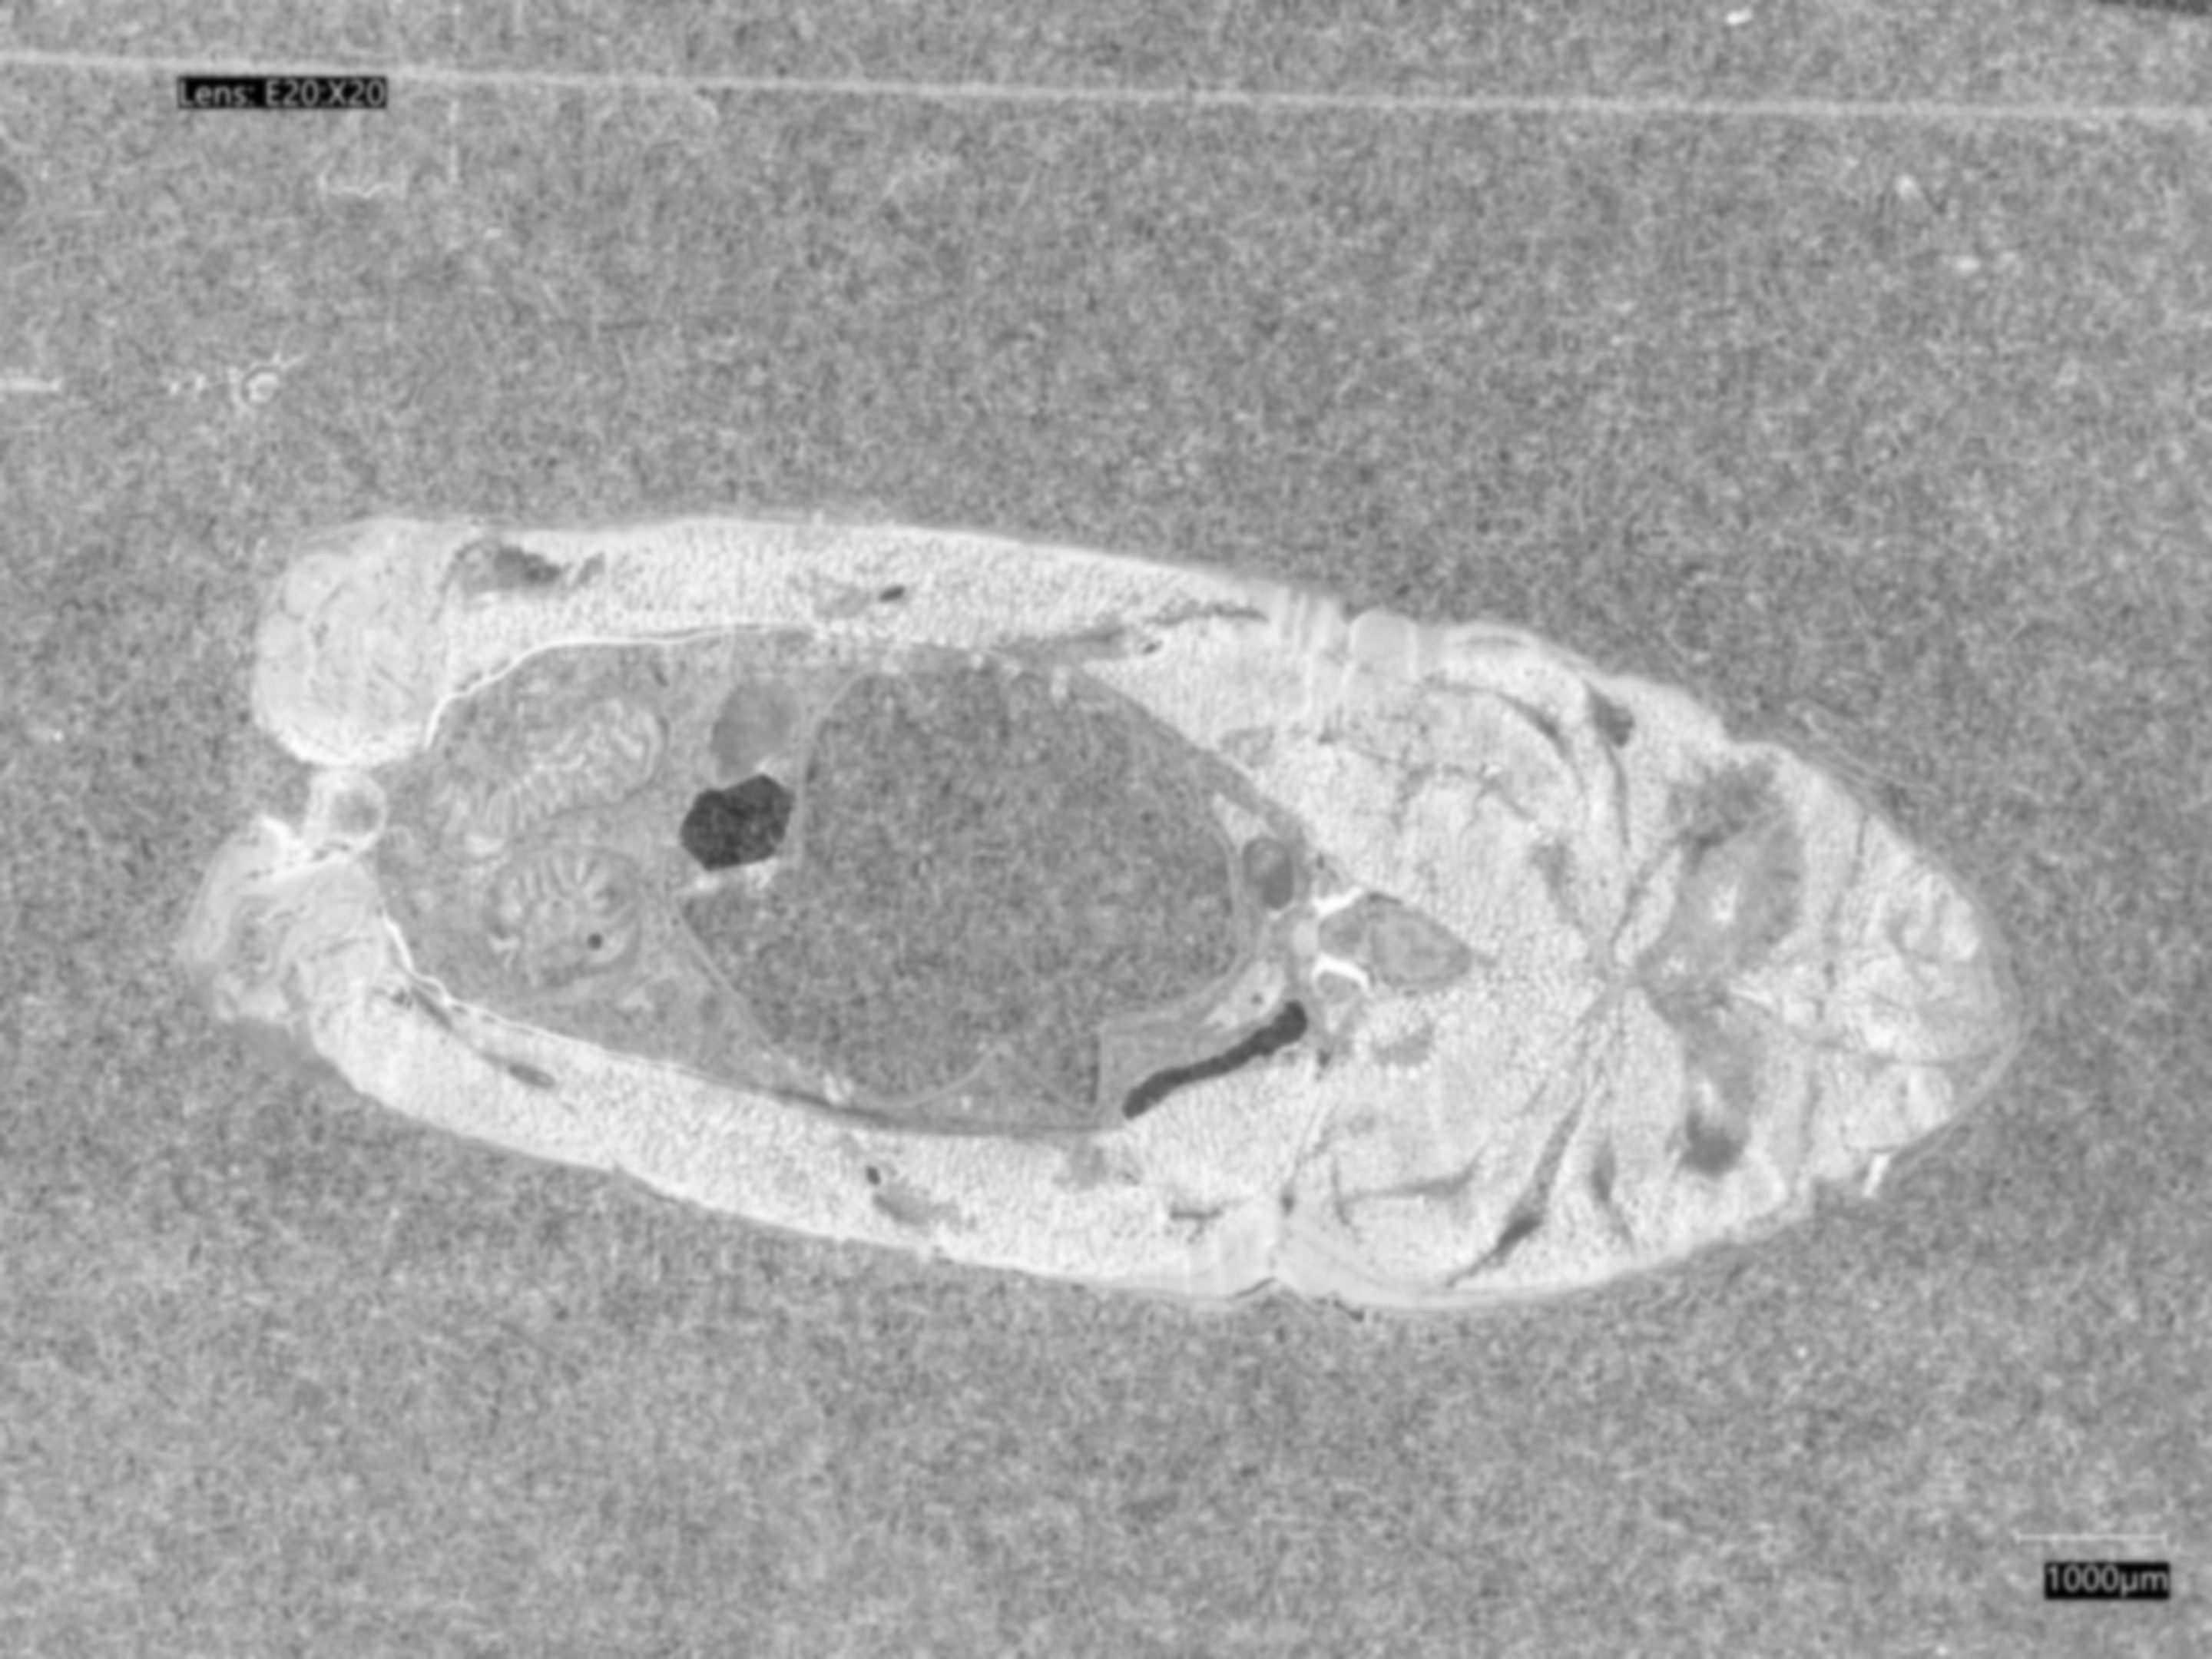
\includegraphics[width=\textwidth]{./fig/gausssian/blurred21.jpg}
        \caption*{k=21}
        \label{fig:blurred21}
    \end{minipage}
    \begin{minipage}{0.24\textwidth}
        \centering
        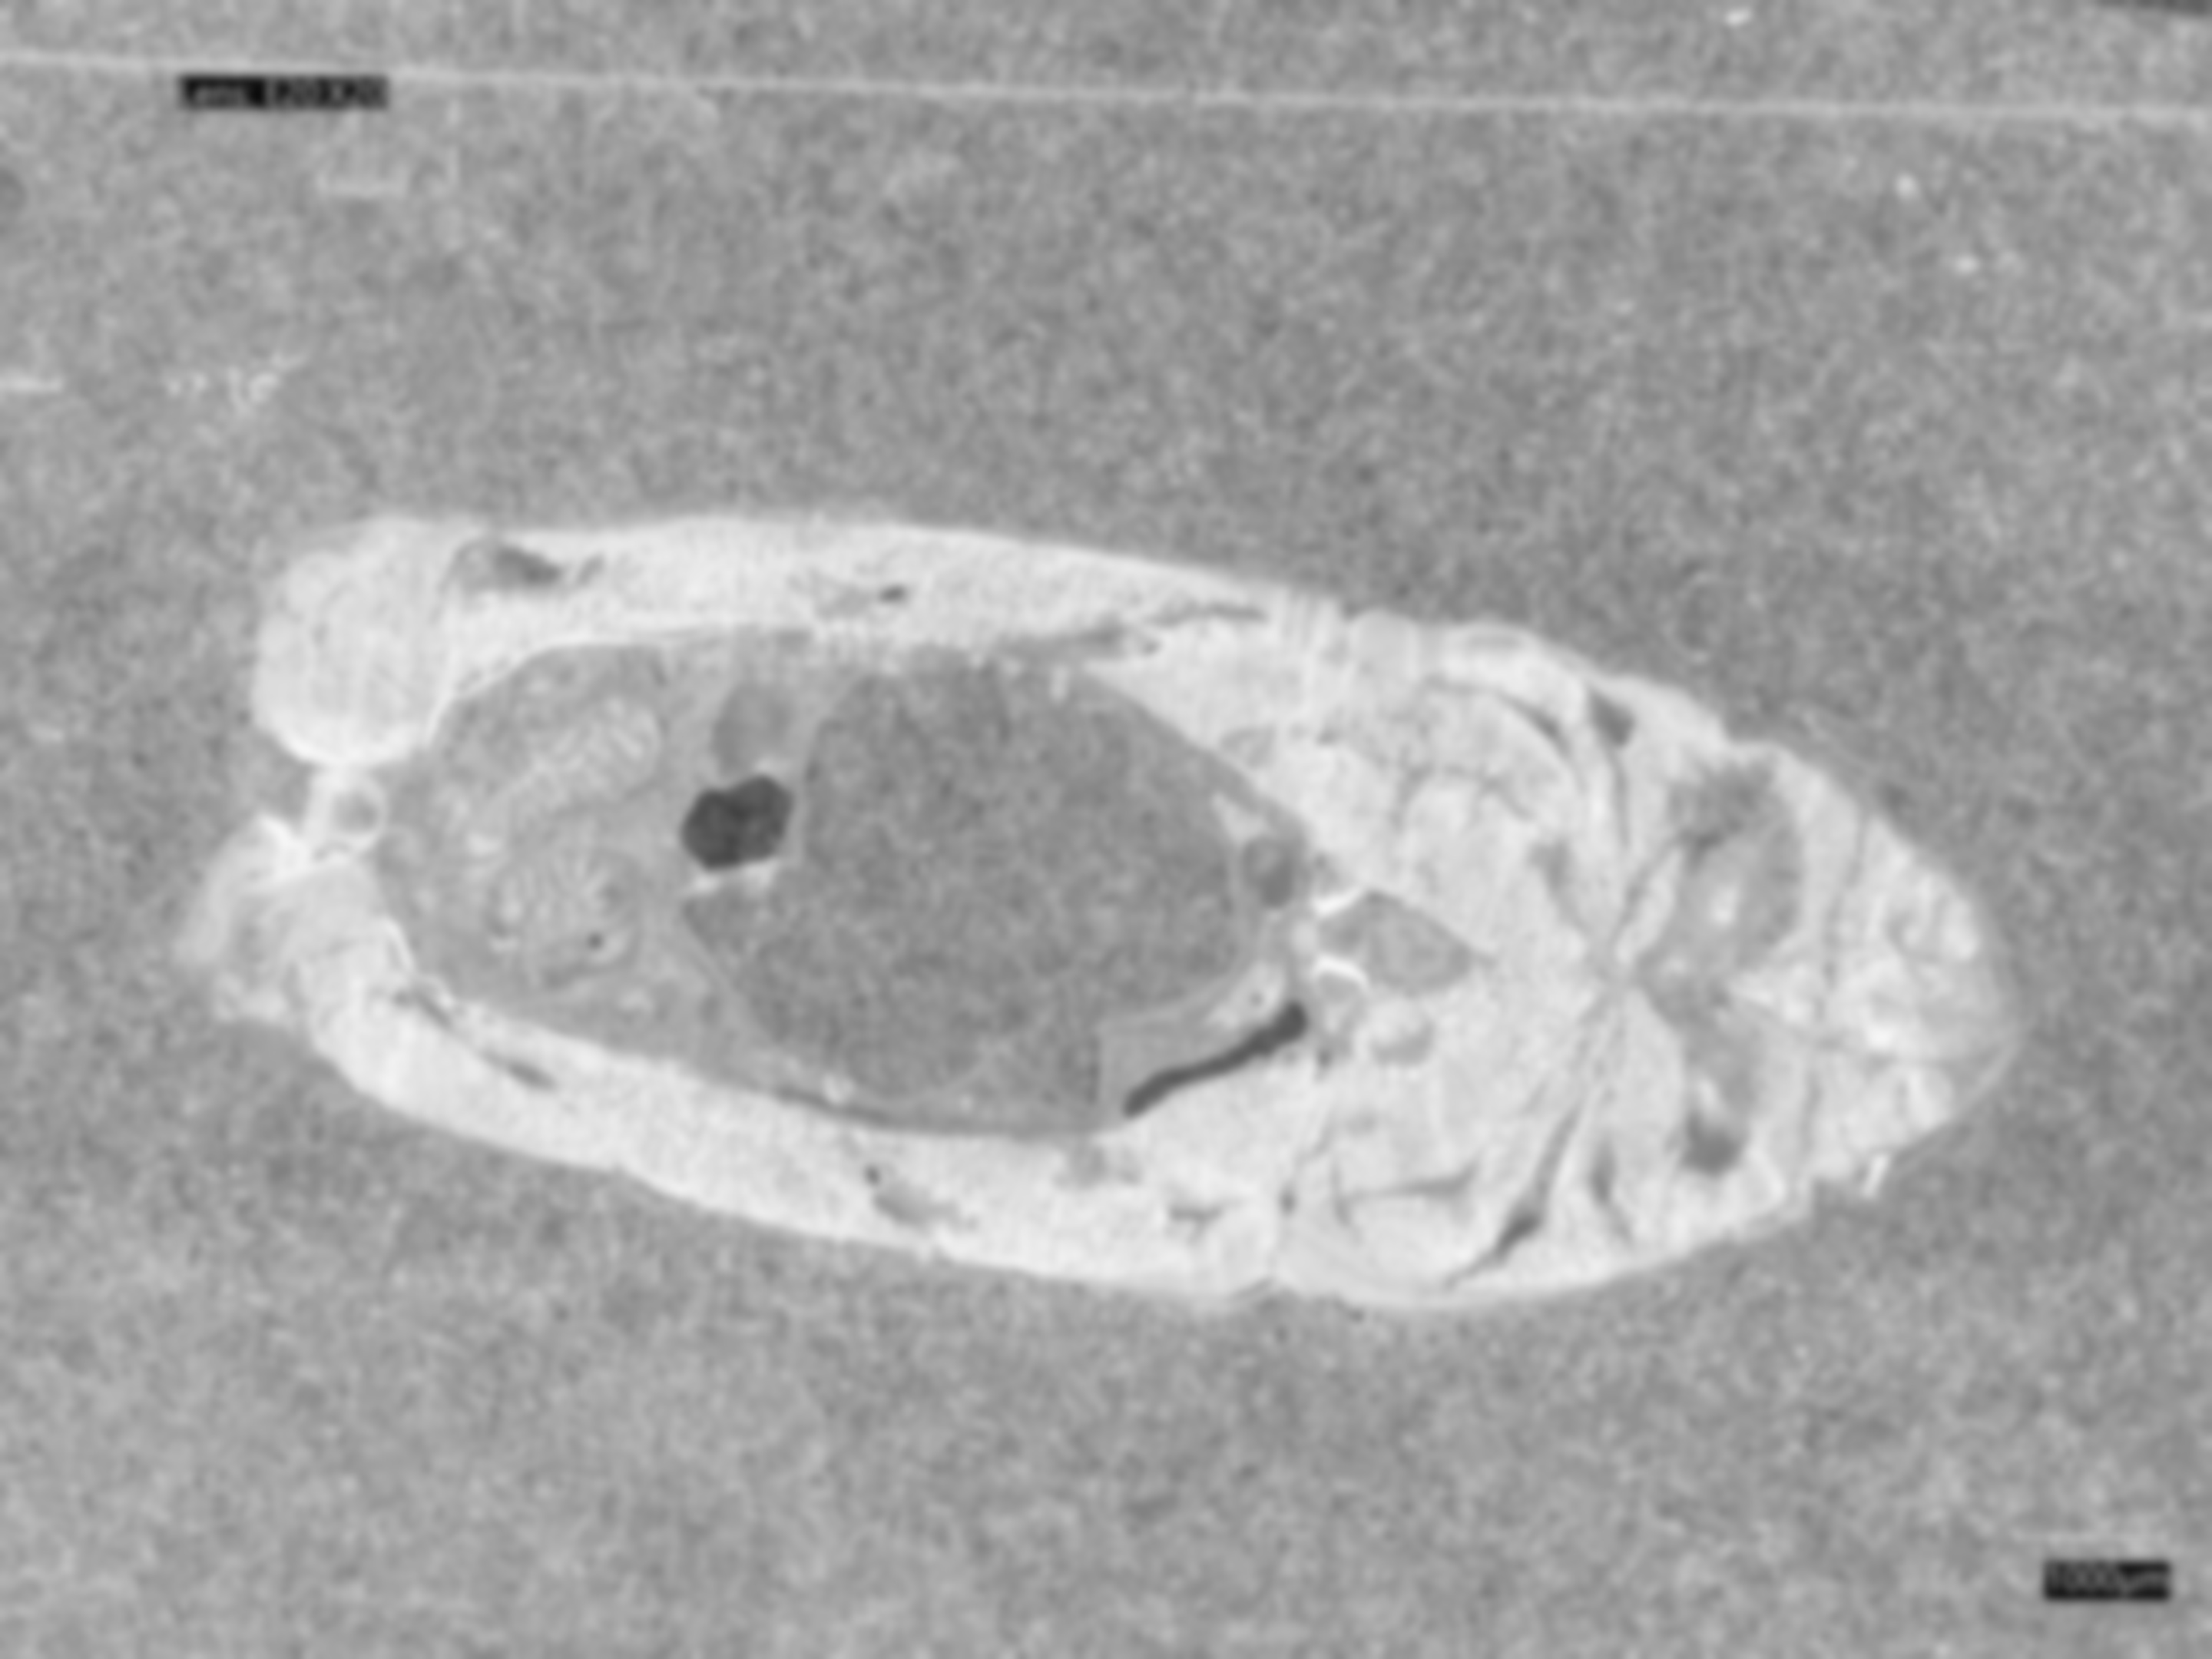
\includegraphics[width=\textwidth]{./fig/gausssian/blurred41.jpg}
        \caption*{k=41}
        \label{fig:blurred41}
    \end{minipage}
    \begin{minipage}{0.24\textwidth}
        \centering
        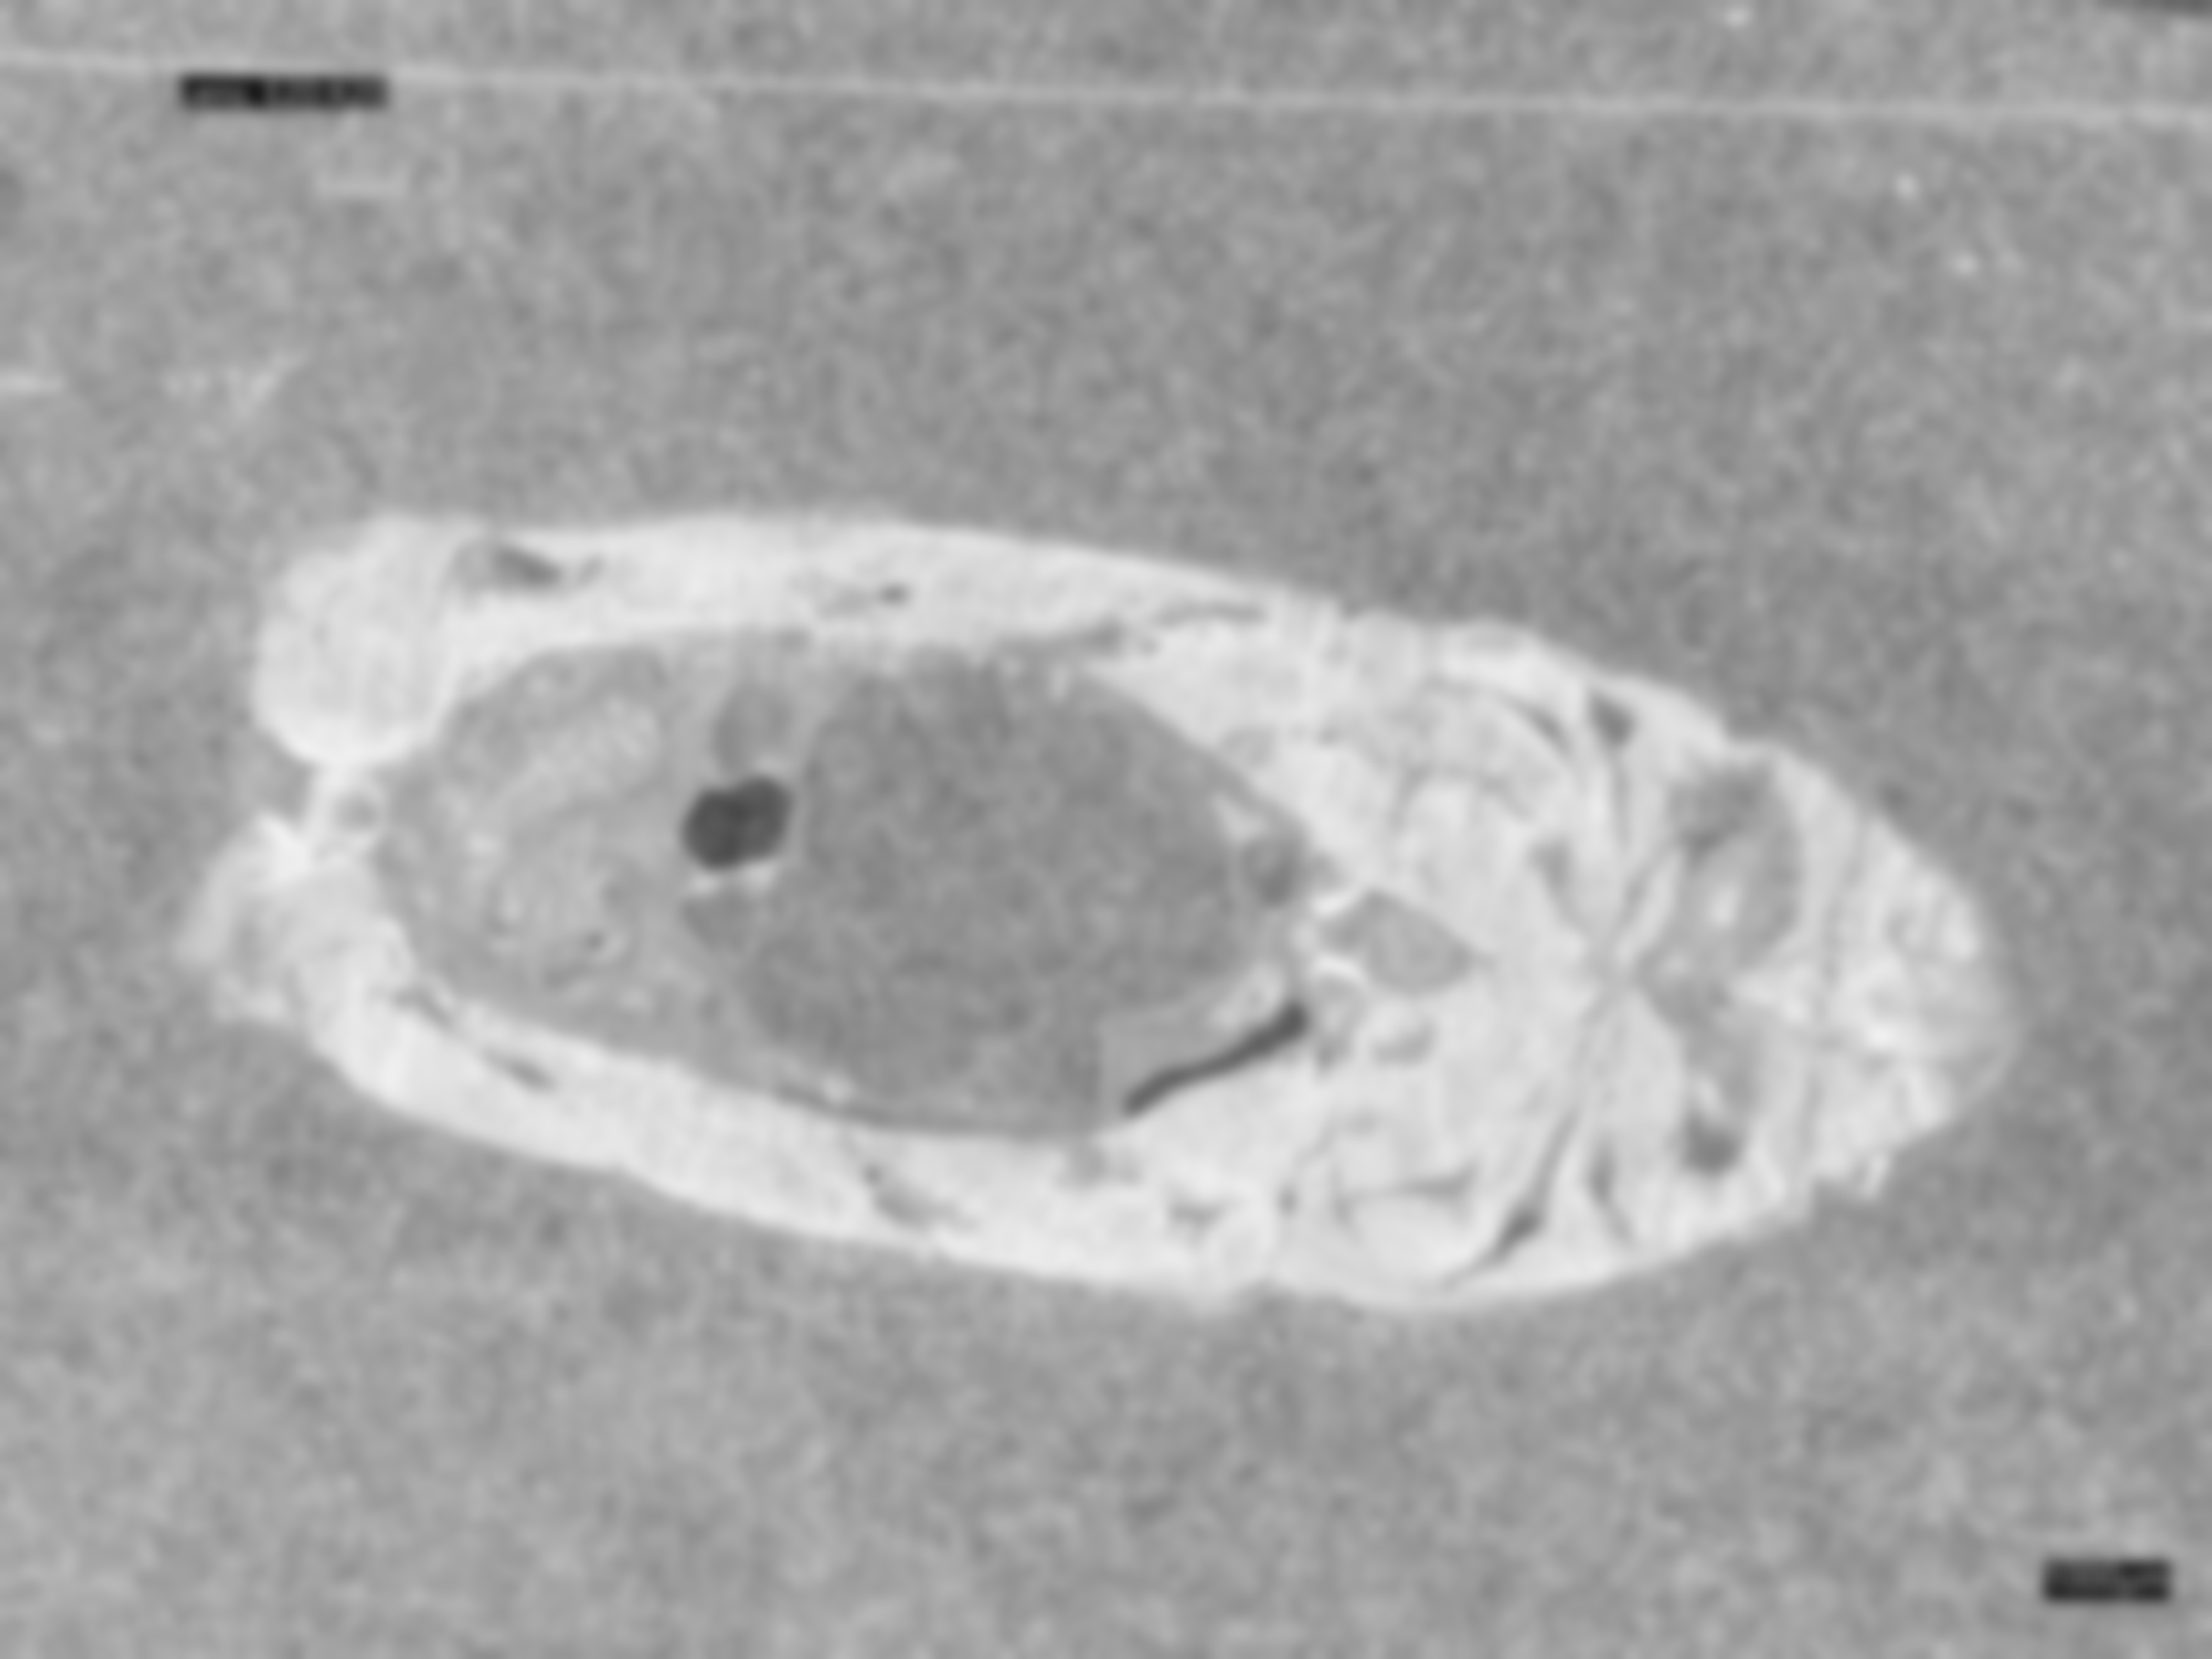
\includegraphics[width=\textwidth]{./fig/gausssian/blurred61.jpg}
        \caption*{k=61}
        \label{fig:blurred61}
    \end{minipage}
    \begin{minipage}{0.24\textwidth}
        \centering
        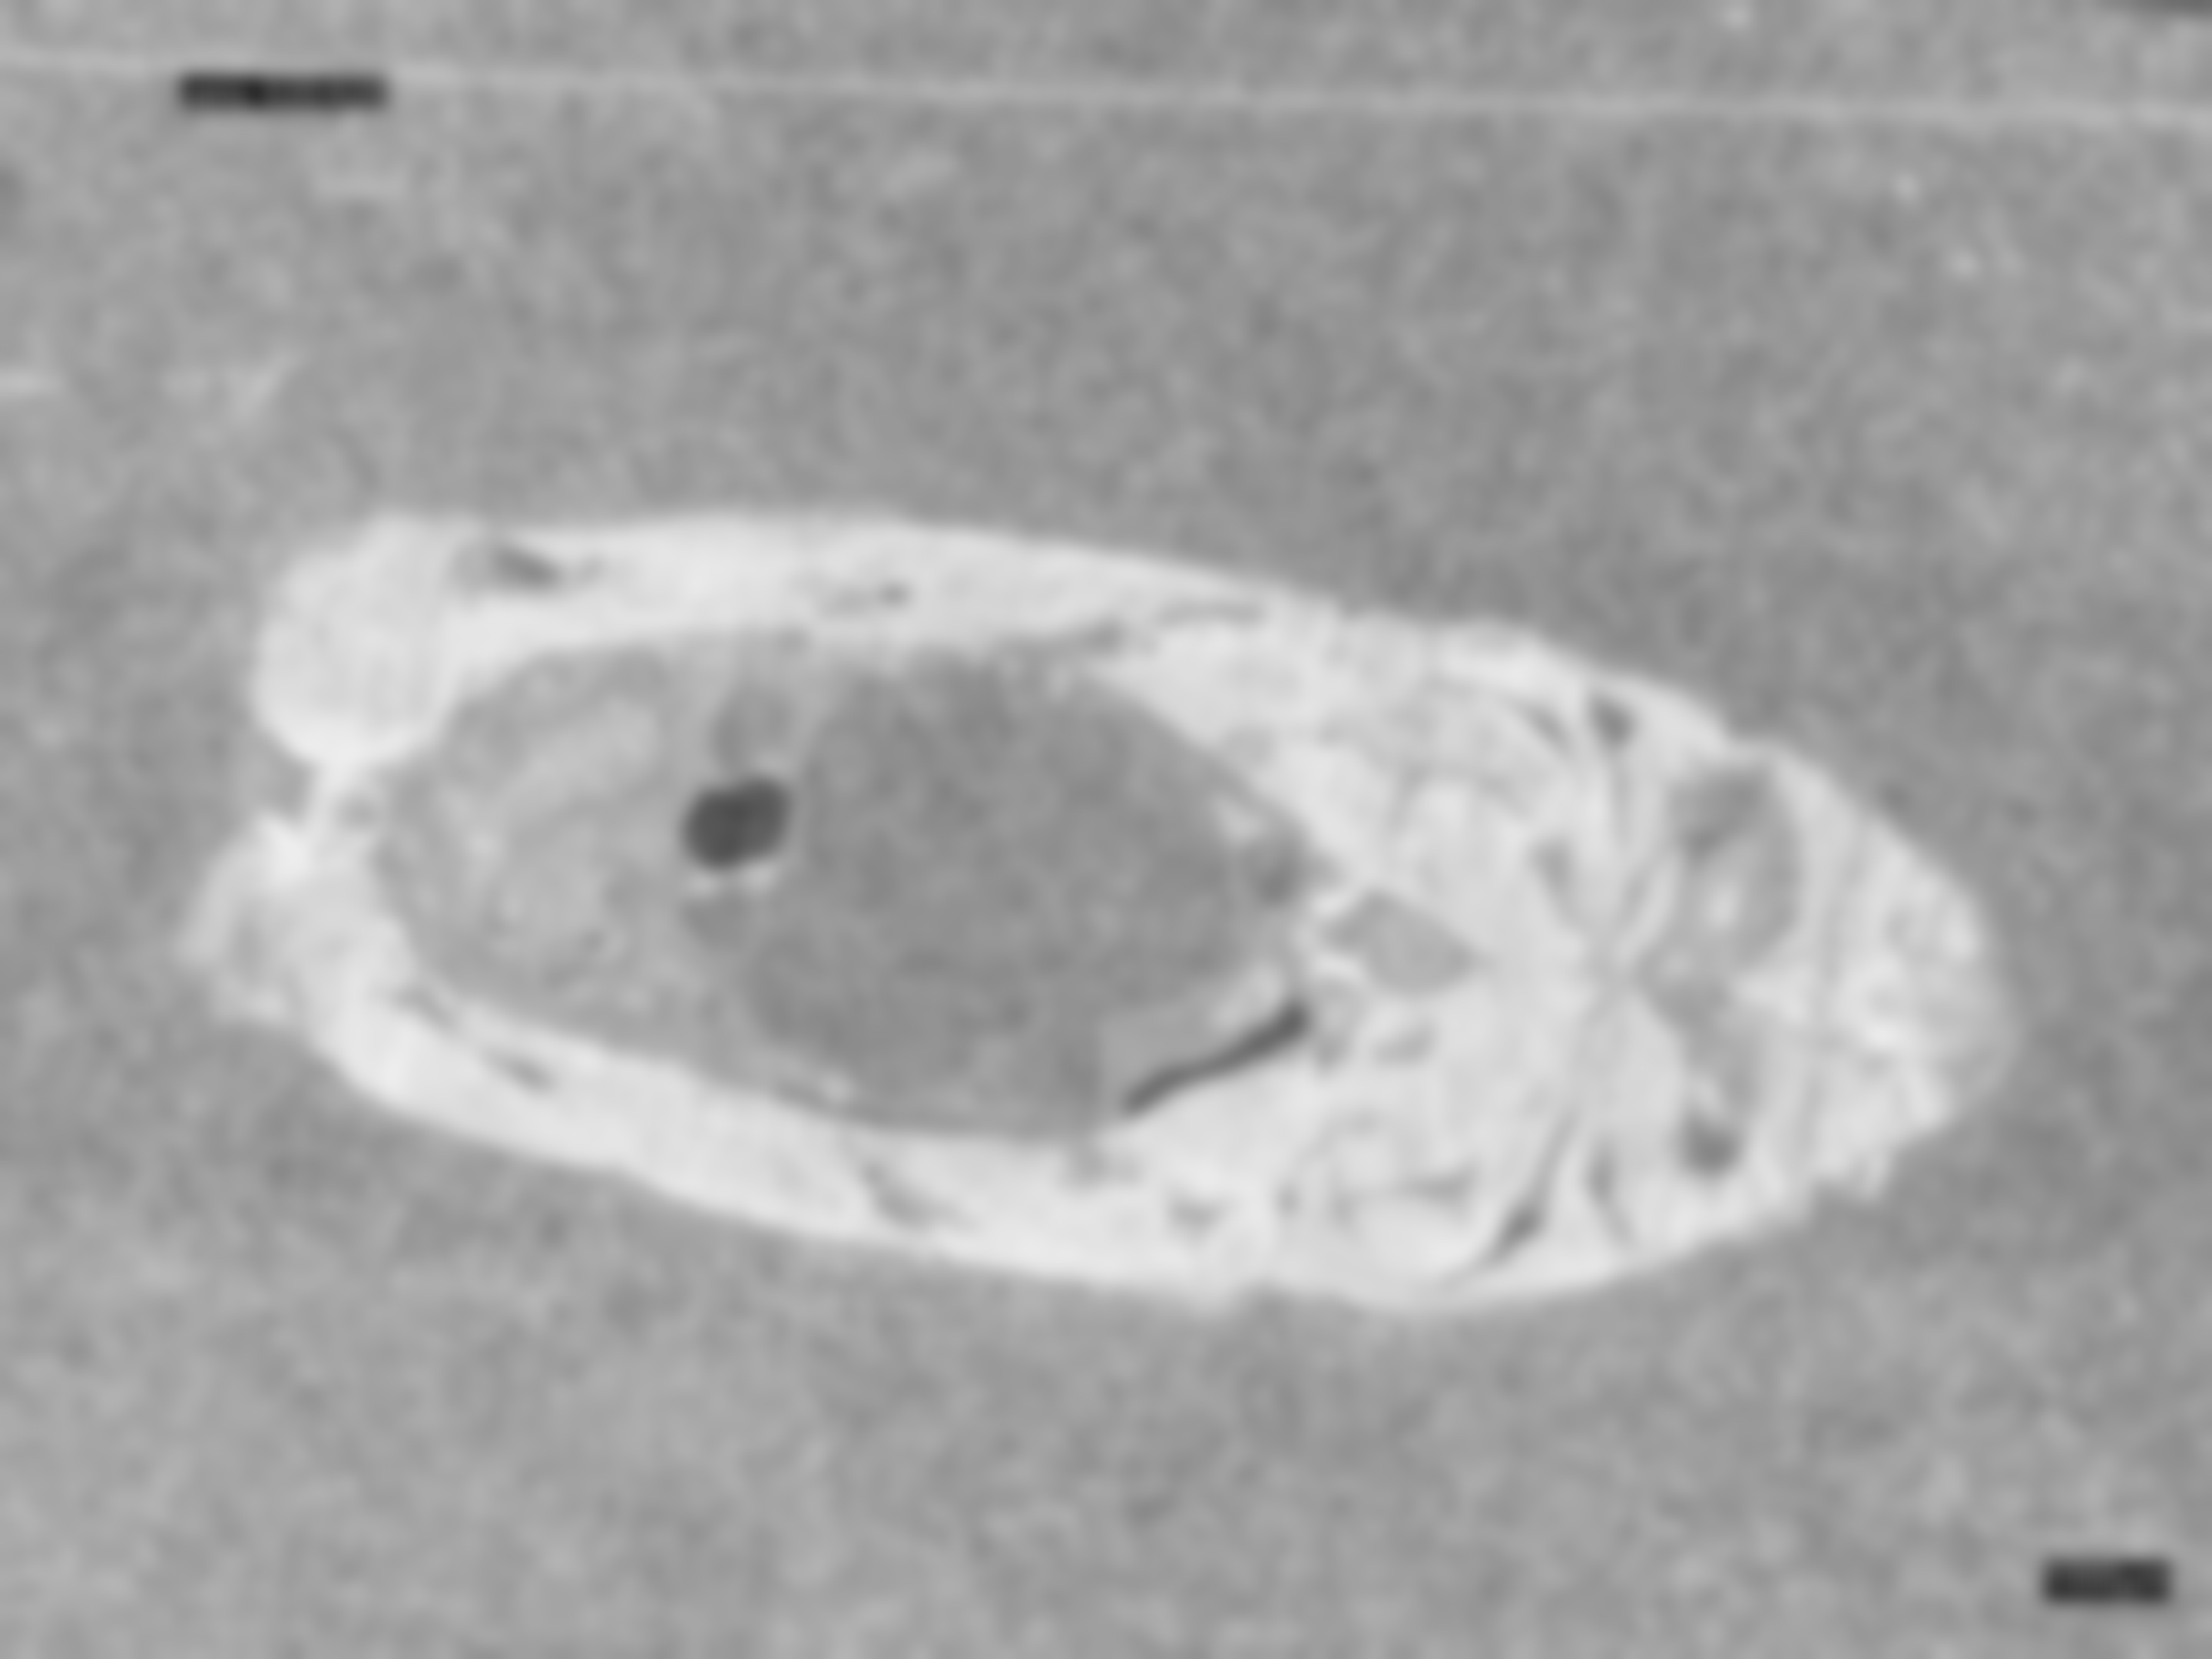
\includegraphics[width=\textwidth]{./fig/gausssian/blurred81.jpg}
        \caption*{k=81}
        \label{fig:blurred81}
    \end{minipage}
    \caption{Images post-Gaussian blur}
    \label{fig:blurred}
\end{figure}

\begin{figure}
    \centering
    \begin{minipage}{0.24\textwidth}
        \centering
        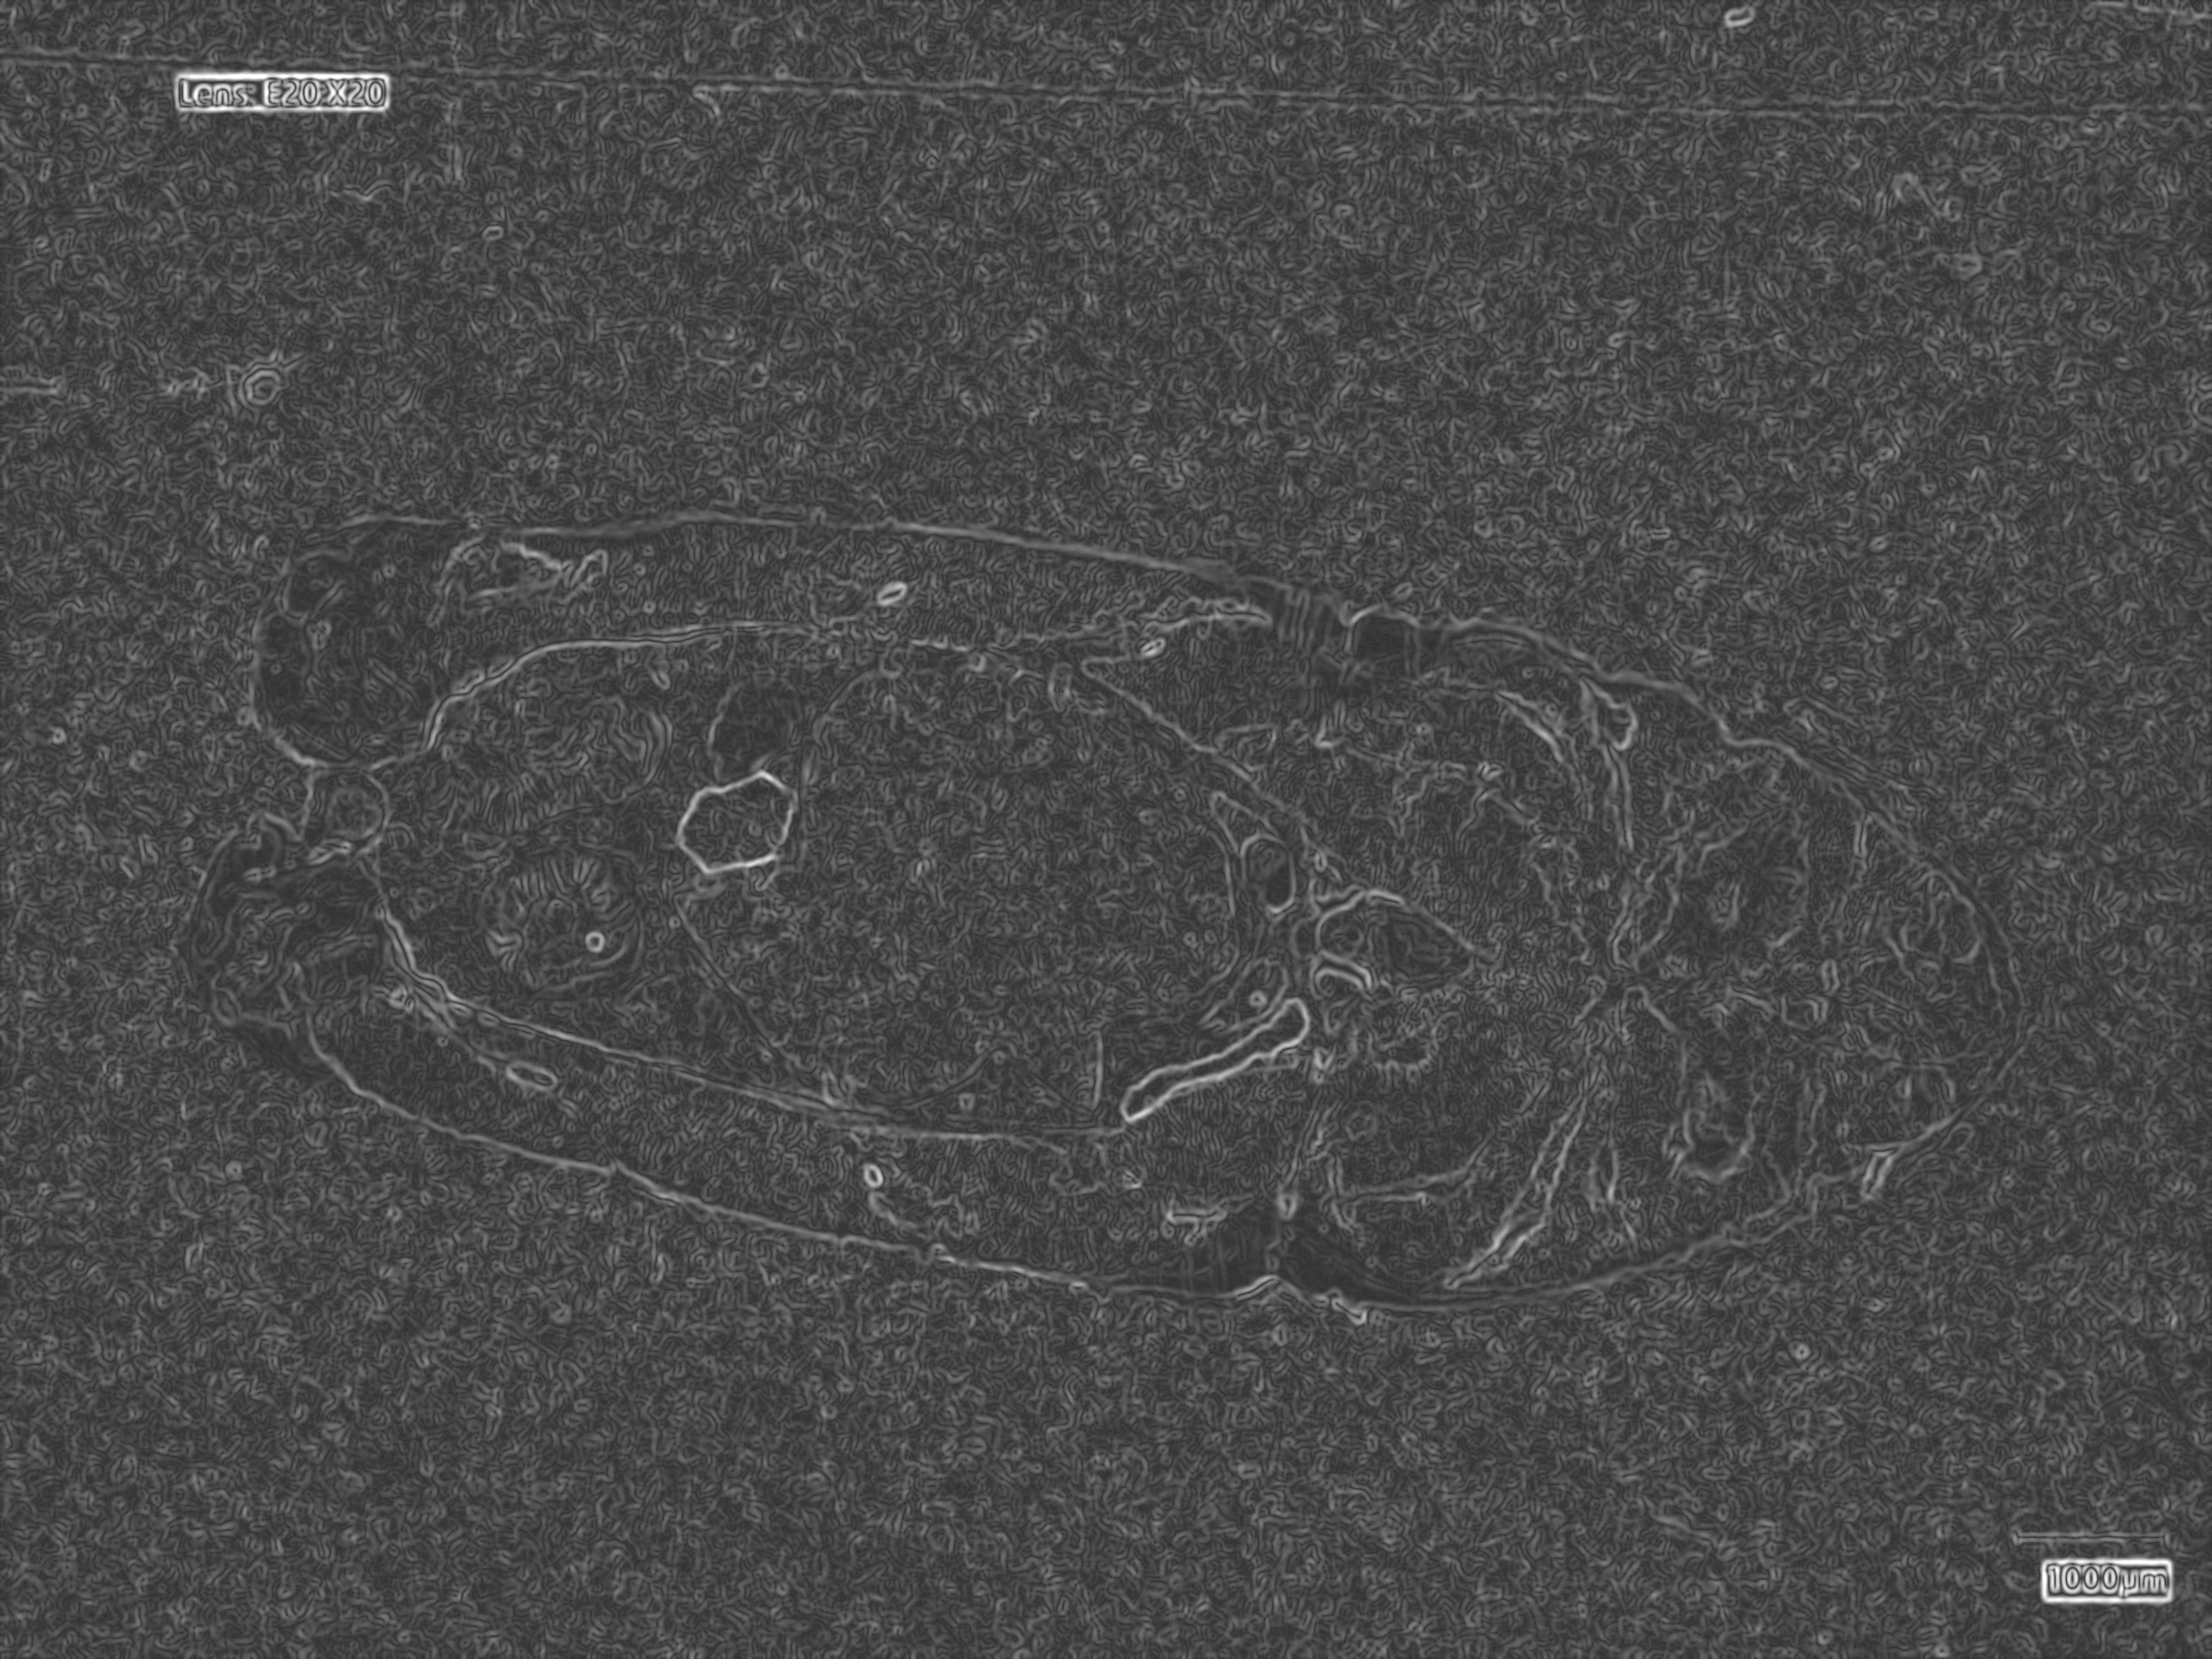
\includegraphics[width=\textwidth]{./fig/gausssian/sobel21.jpg}
        \caption*{k=21}
        \label{fig:sobel21}
    \end{minipage}
    \begin{minipage}{0.24\textwidth}
        \centering
        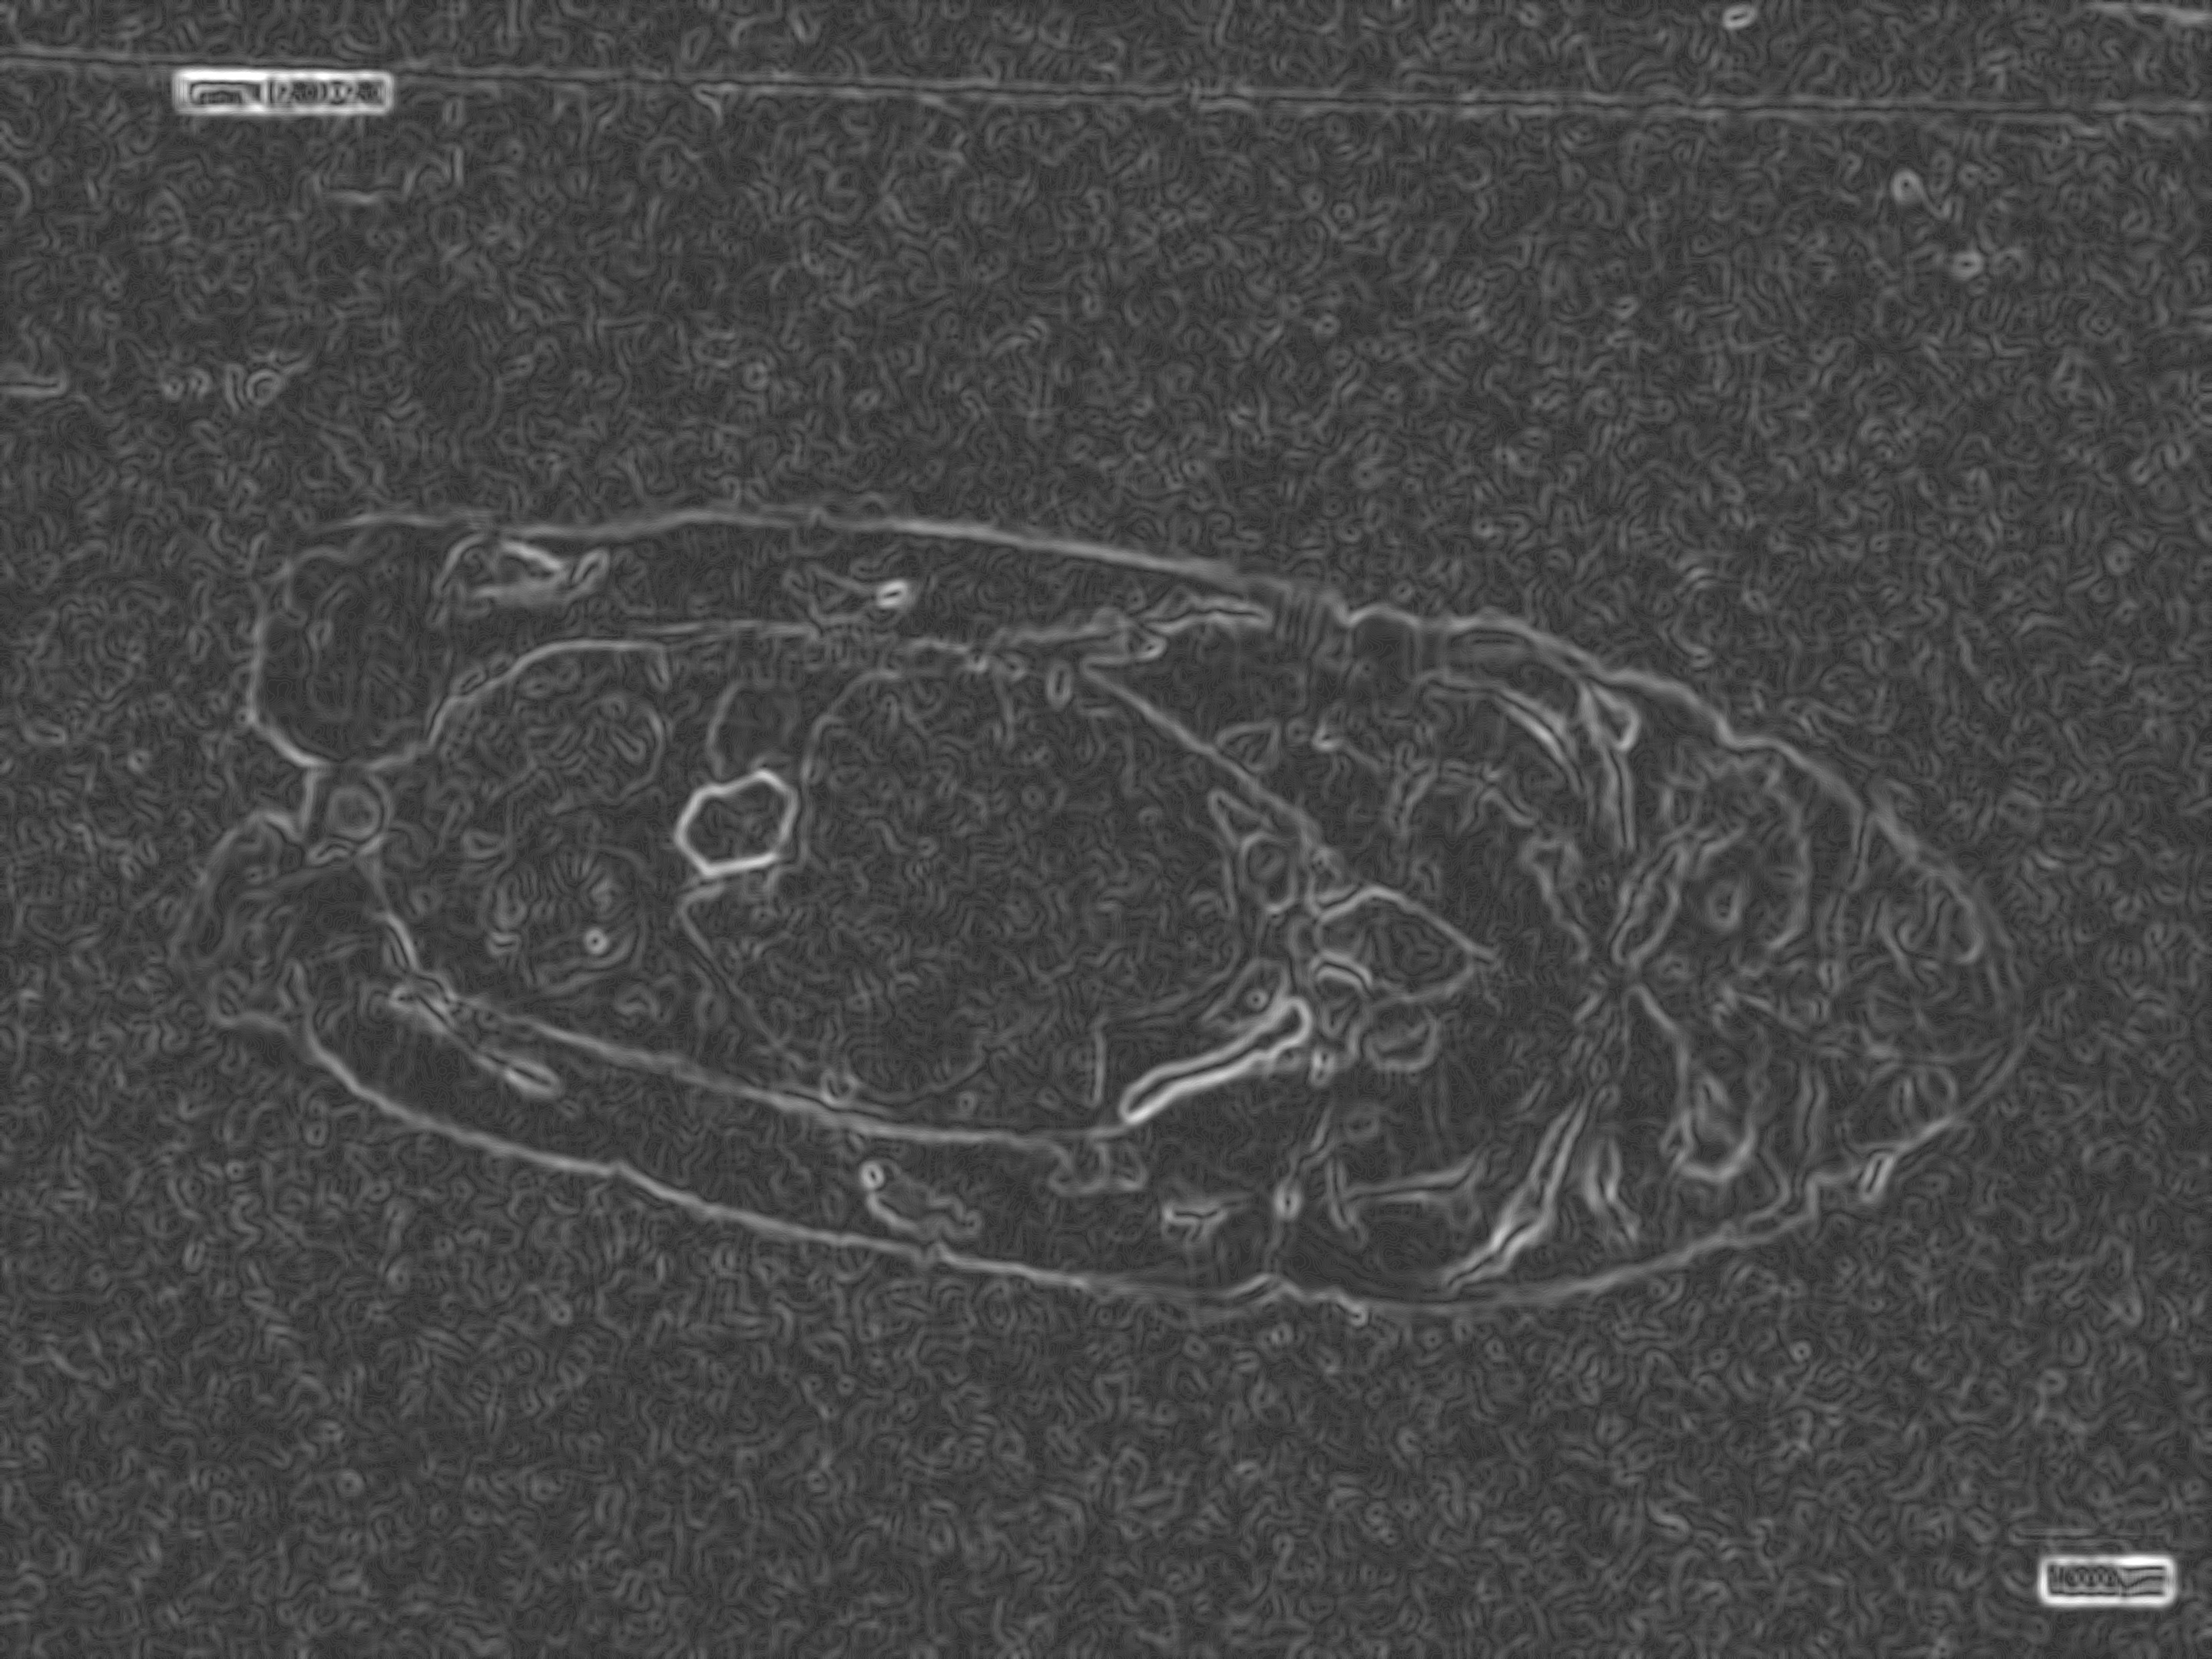
\includegraphics[width=\textwidth]{./fig/gausssian/sobel41.jpg}
        \caption*{k=41}
        \label{fig:sobel41}
    \end{minipage}
    \begin{minipage}{0.24\textwidth}
        \centering
        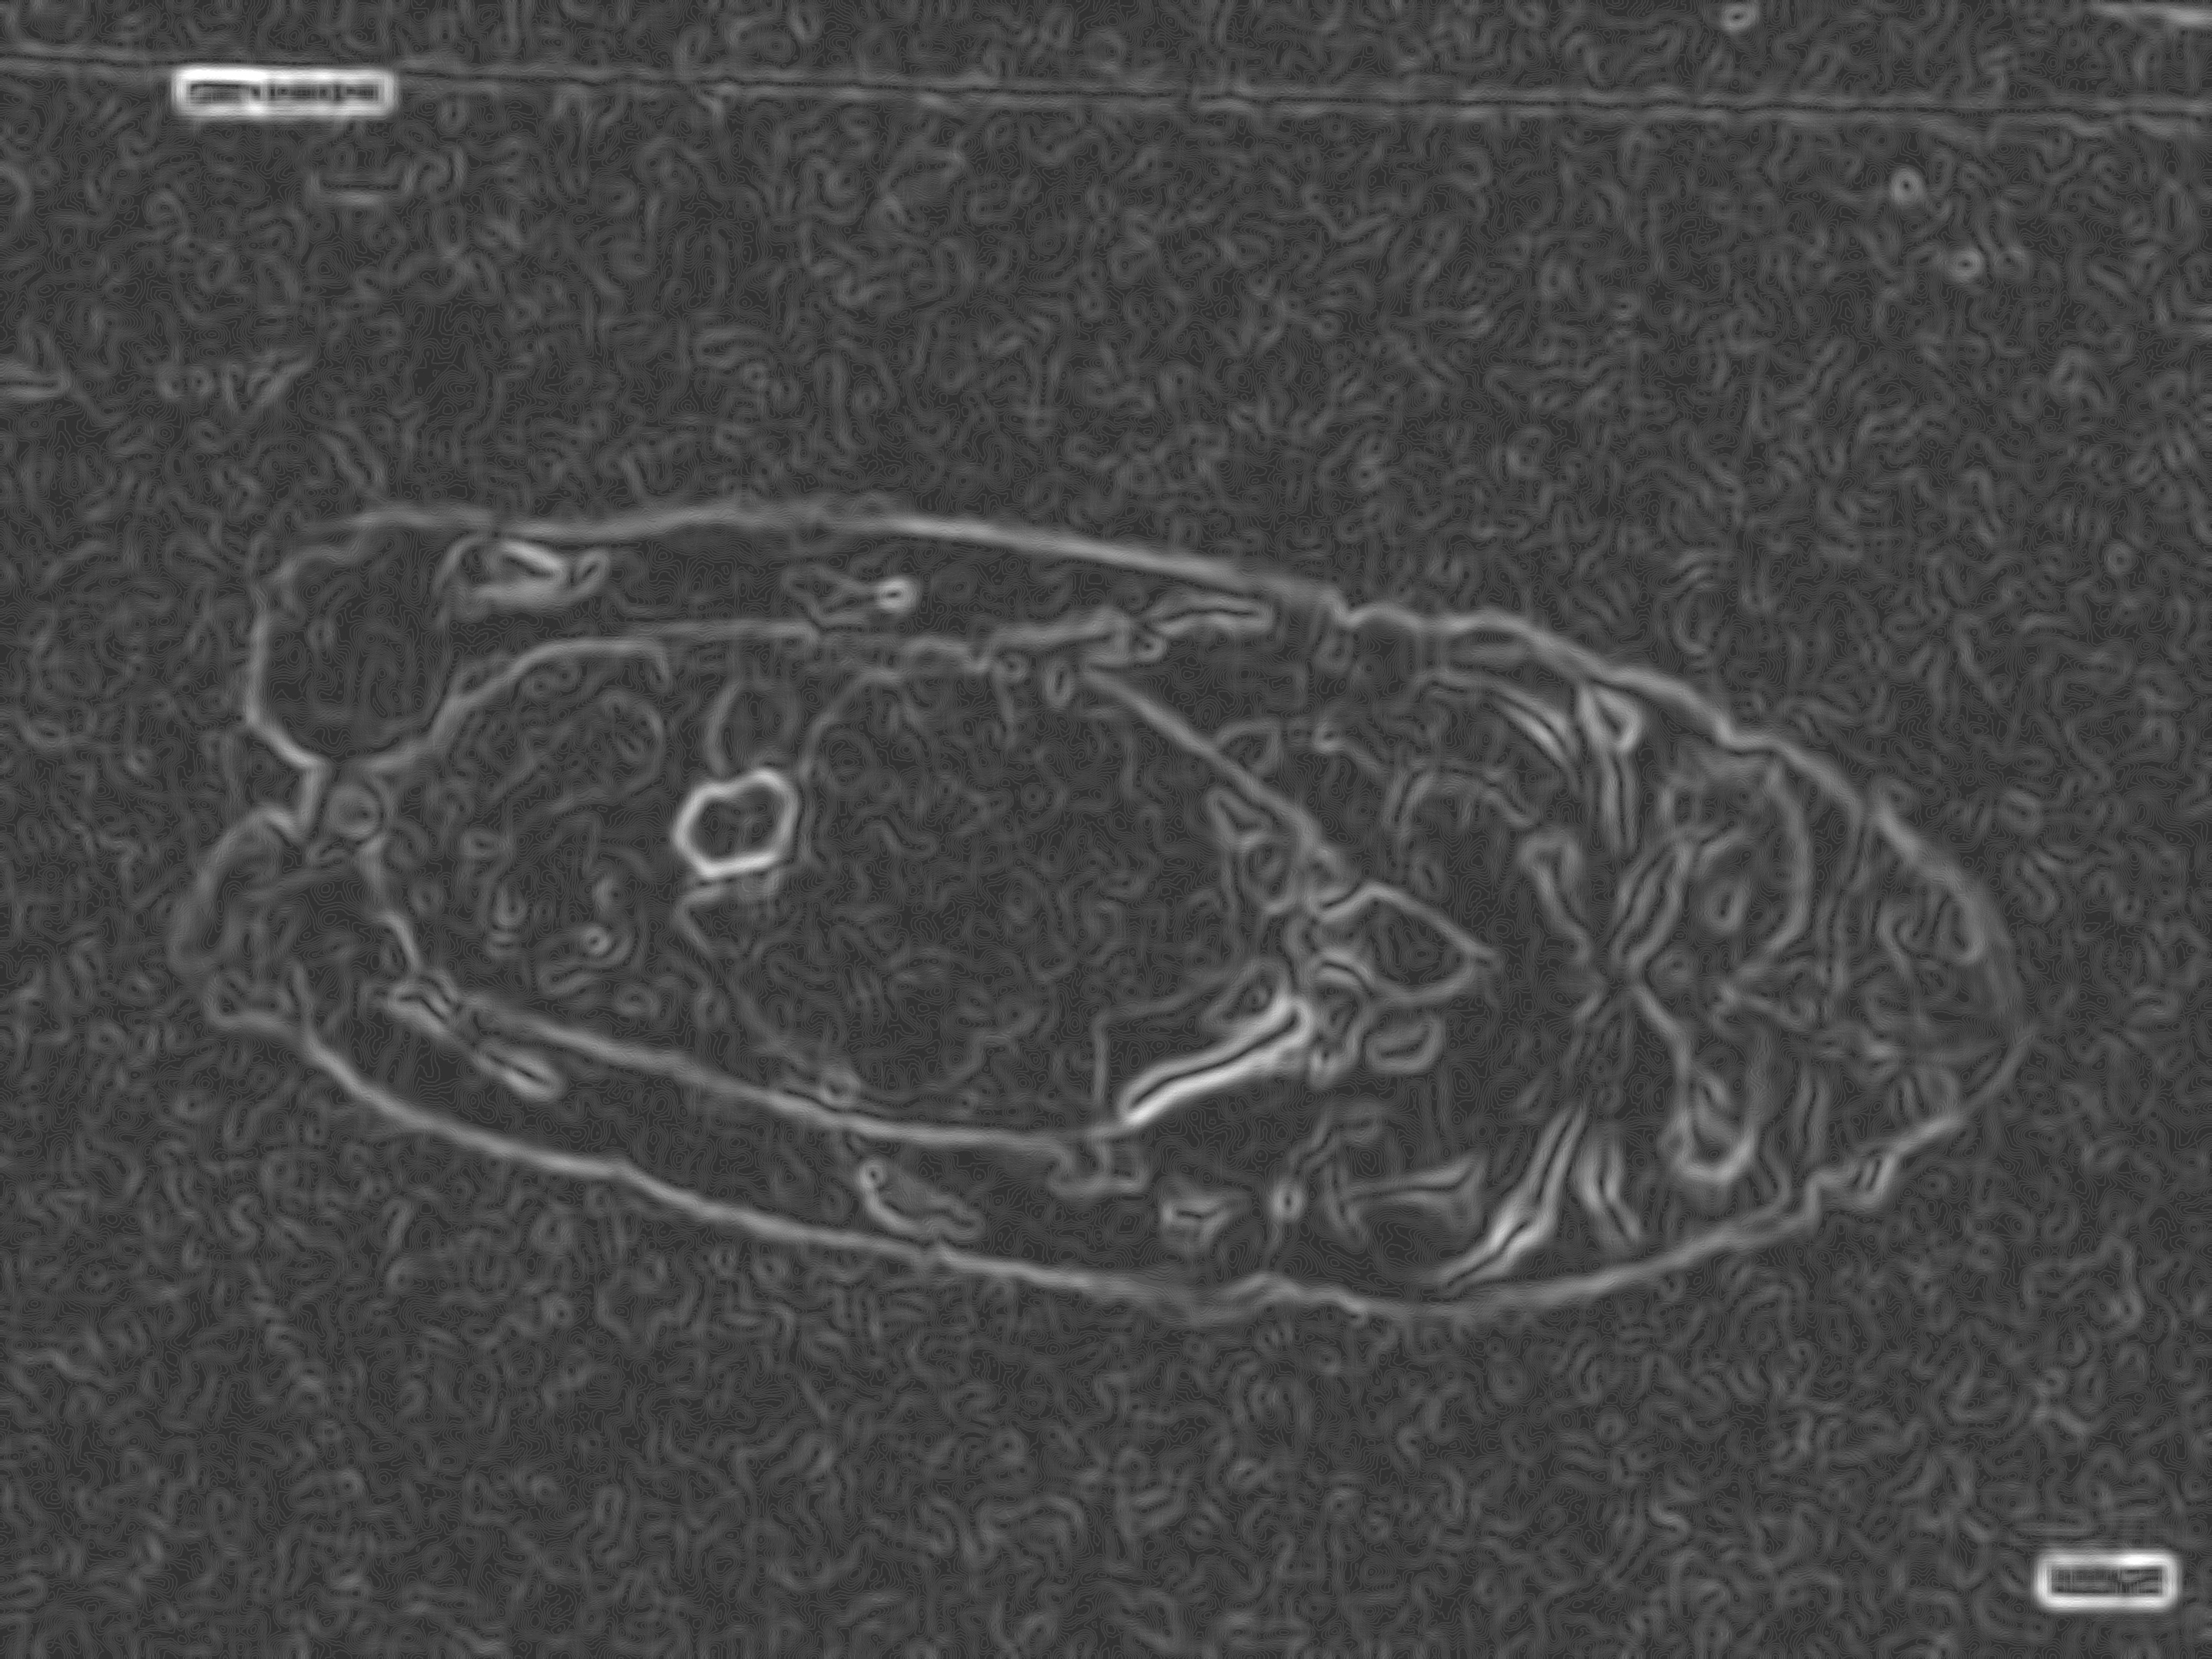
\includegraphics[width=\textwidth]{./fig/gausssian/sobel61.jpg}
        \caption*{k=61}
        \label{fig:sobel61}
    \end{minipage}
    \begin{minipage}{0.24\textwidth}
        \centering
        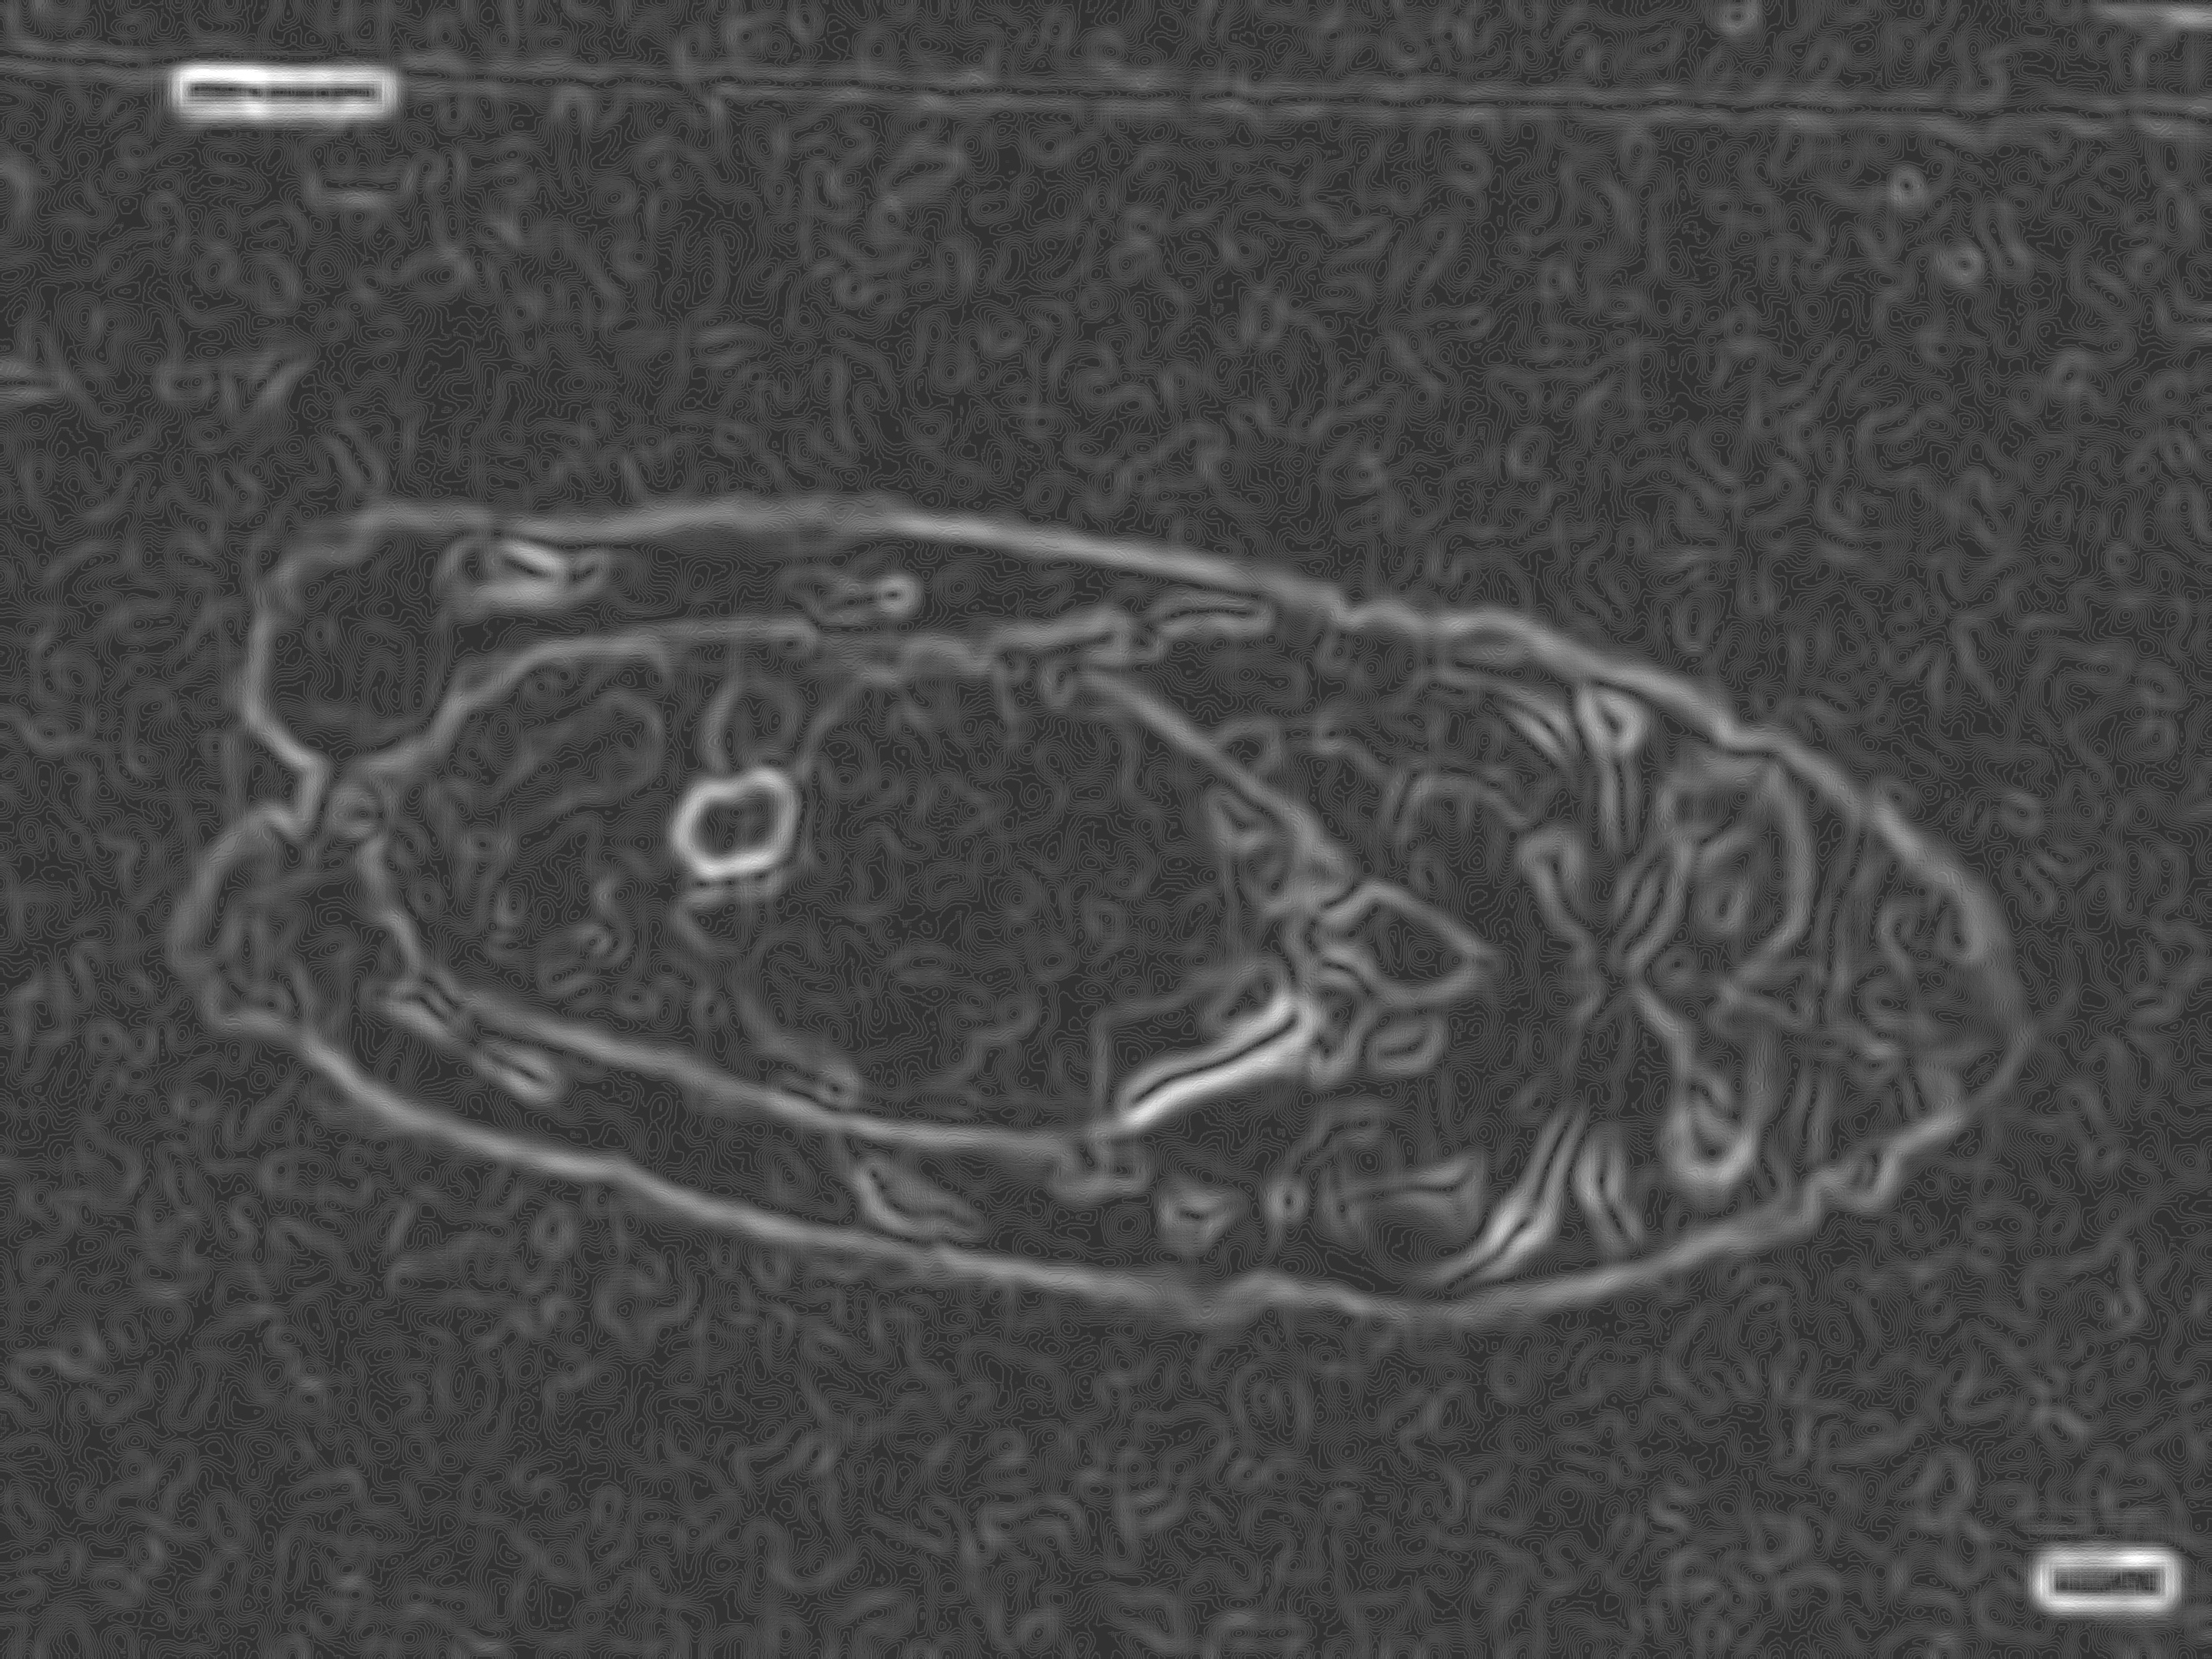
\includegraphics[width=\textwidth]{./fig/gausssian/sobel81.jpg}
        \caption*{k=81}
        \label{fig:sobel81}
    \end{minipage}
    \caption{Images post-Sobel operator}
    \label{fig:sobel}
\end{figure}


在\autoref{fig:blurred}中,可以观察到,随着高斯模糊核大小的增加,图像细节逐渐变得更加模糊,边缘也变得更加不明显。在\autoref{fig:sobel}中,随着核大小的增加,边缘检测的有效性减弱,边缘变得不那么突出。考虑到图像边缘与背景噪声的清晰度,选择了61的高斯核大小。

以下是在高斯模糊(k=61)后使用python的opencv库执行laplacian算子的结果。

\begin{figure}[H]
    \centering
    \begin{minipage}{0.4\textwidth}
        \centering
        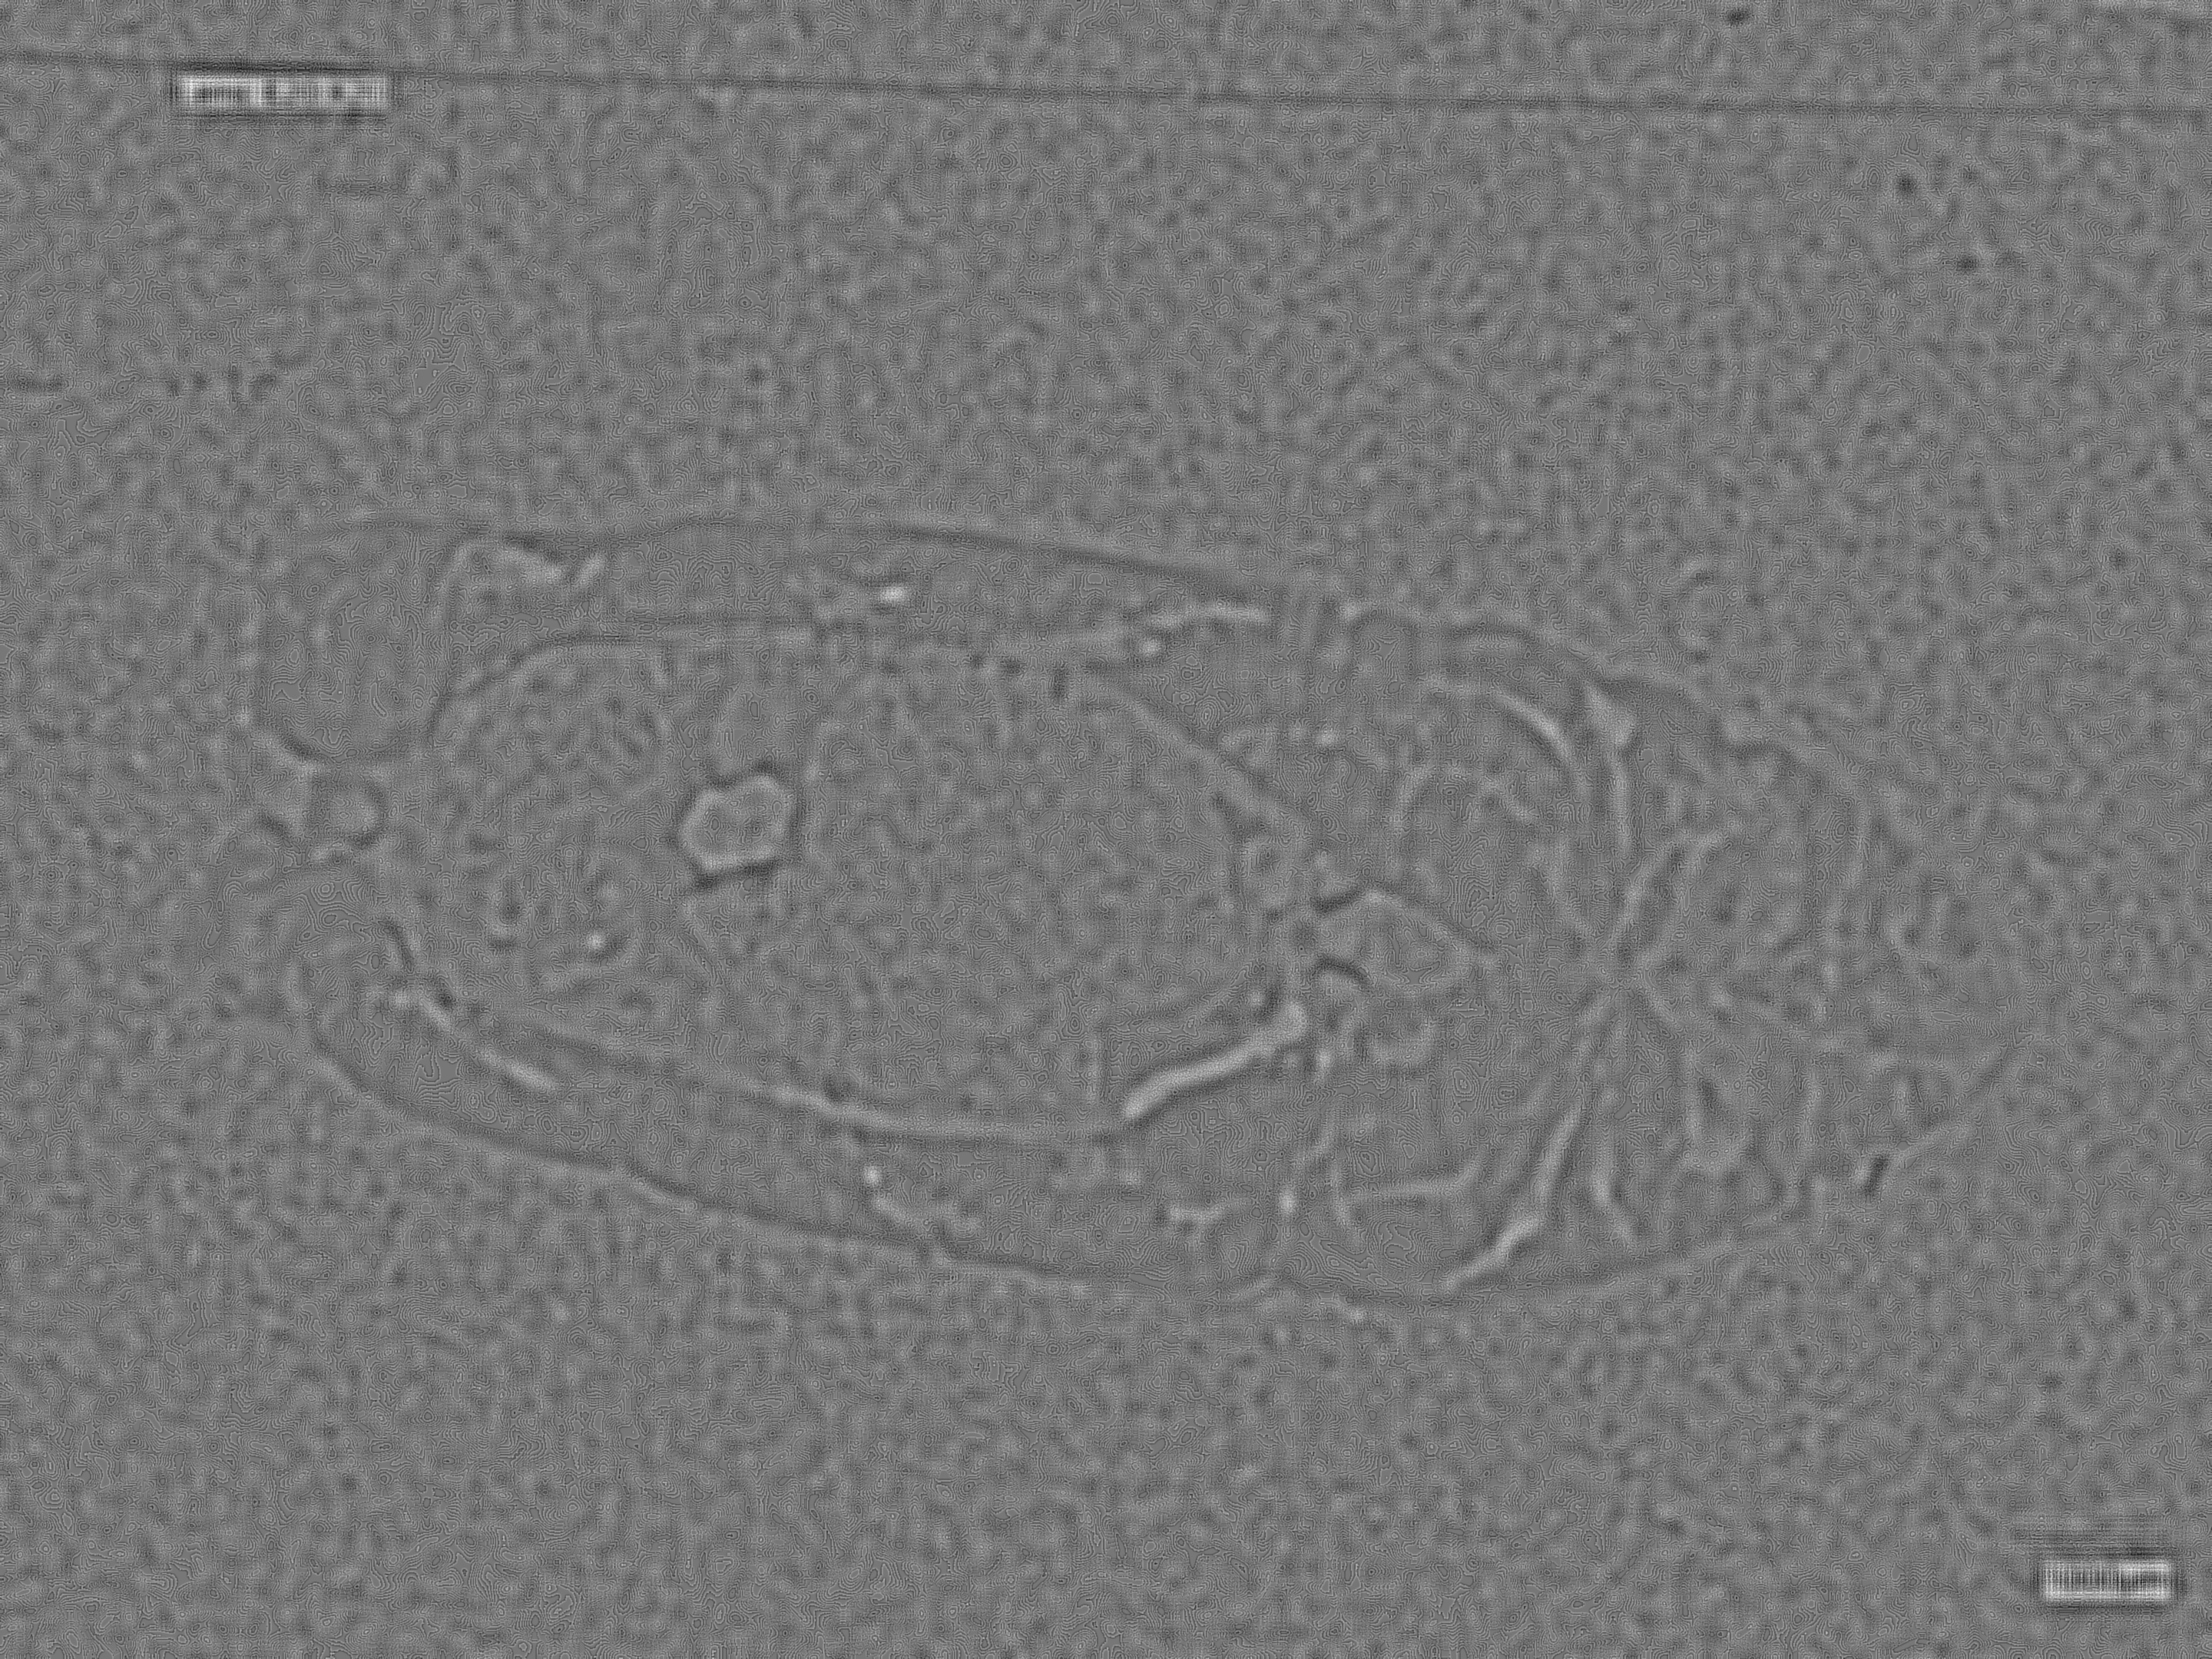
\includegraphics[width=\textwidth]{./fig/gausssian/laplacian61.jpg}
        \caption{laplacian}
        \label{fig:laplacian}
    \end{minipage}
\end{figure}

同样在3.1.1节提到的,canny算法相对于sobel算法稍显复杂-引入了阈值检测,非极大值抑制等步骤。canny算法引入了两个阈值,分别为低阈值和高阈值。其中,当图像的梯度值大于高阈值时,被认为是边缘;当图像的梯度值小于低阈值时,被认为不是边缘;当图像的梯度值在两者之间时,如果与高阈值的边缘相连,则被认为是边缘,否则被认为不是边缘。这样的处理可以有效的去除图像中的噪声,得到更加准确的边缘检测结果。

通常情况下,高阈值和低阈值的比值在2:1到3:1之间。在这里我们选择阈值比为2.5 : 1,探究不同阈值对边缘检测的影响。

取低阈值为2 4 6 ,此时对应的高阈值为5 10 15 。canny算法的结果如下所示。

\begin{figure}
    \centering
    \begin{minipage}{0.32\textwidth}
        \centering
        \includegraphics[width=\textwidth]{./fig/gausssian/canny61+2.jpg}
        \caption{canny 2 5}
        \label{fig:canny2_5}
    \end{minipage}
    \begin{minipage}{0.32\textwidth}
        \centering
        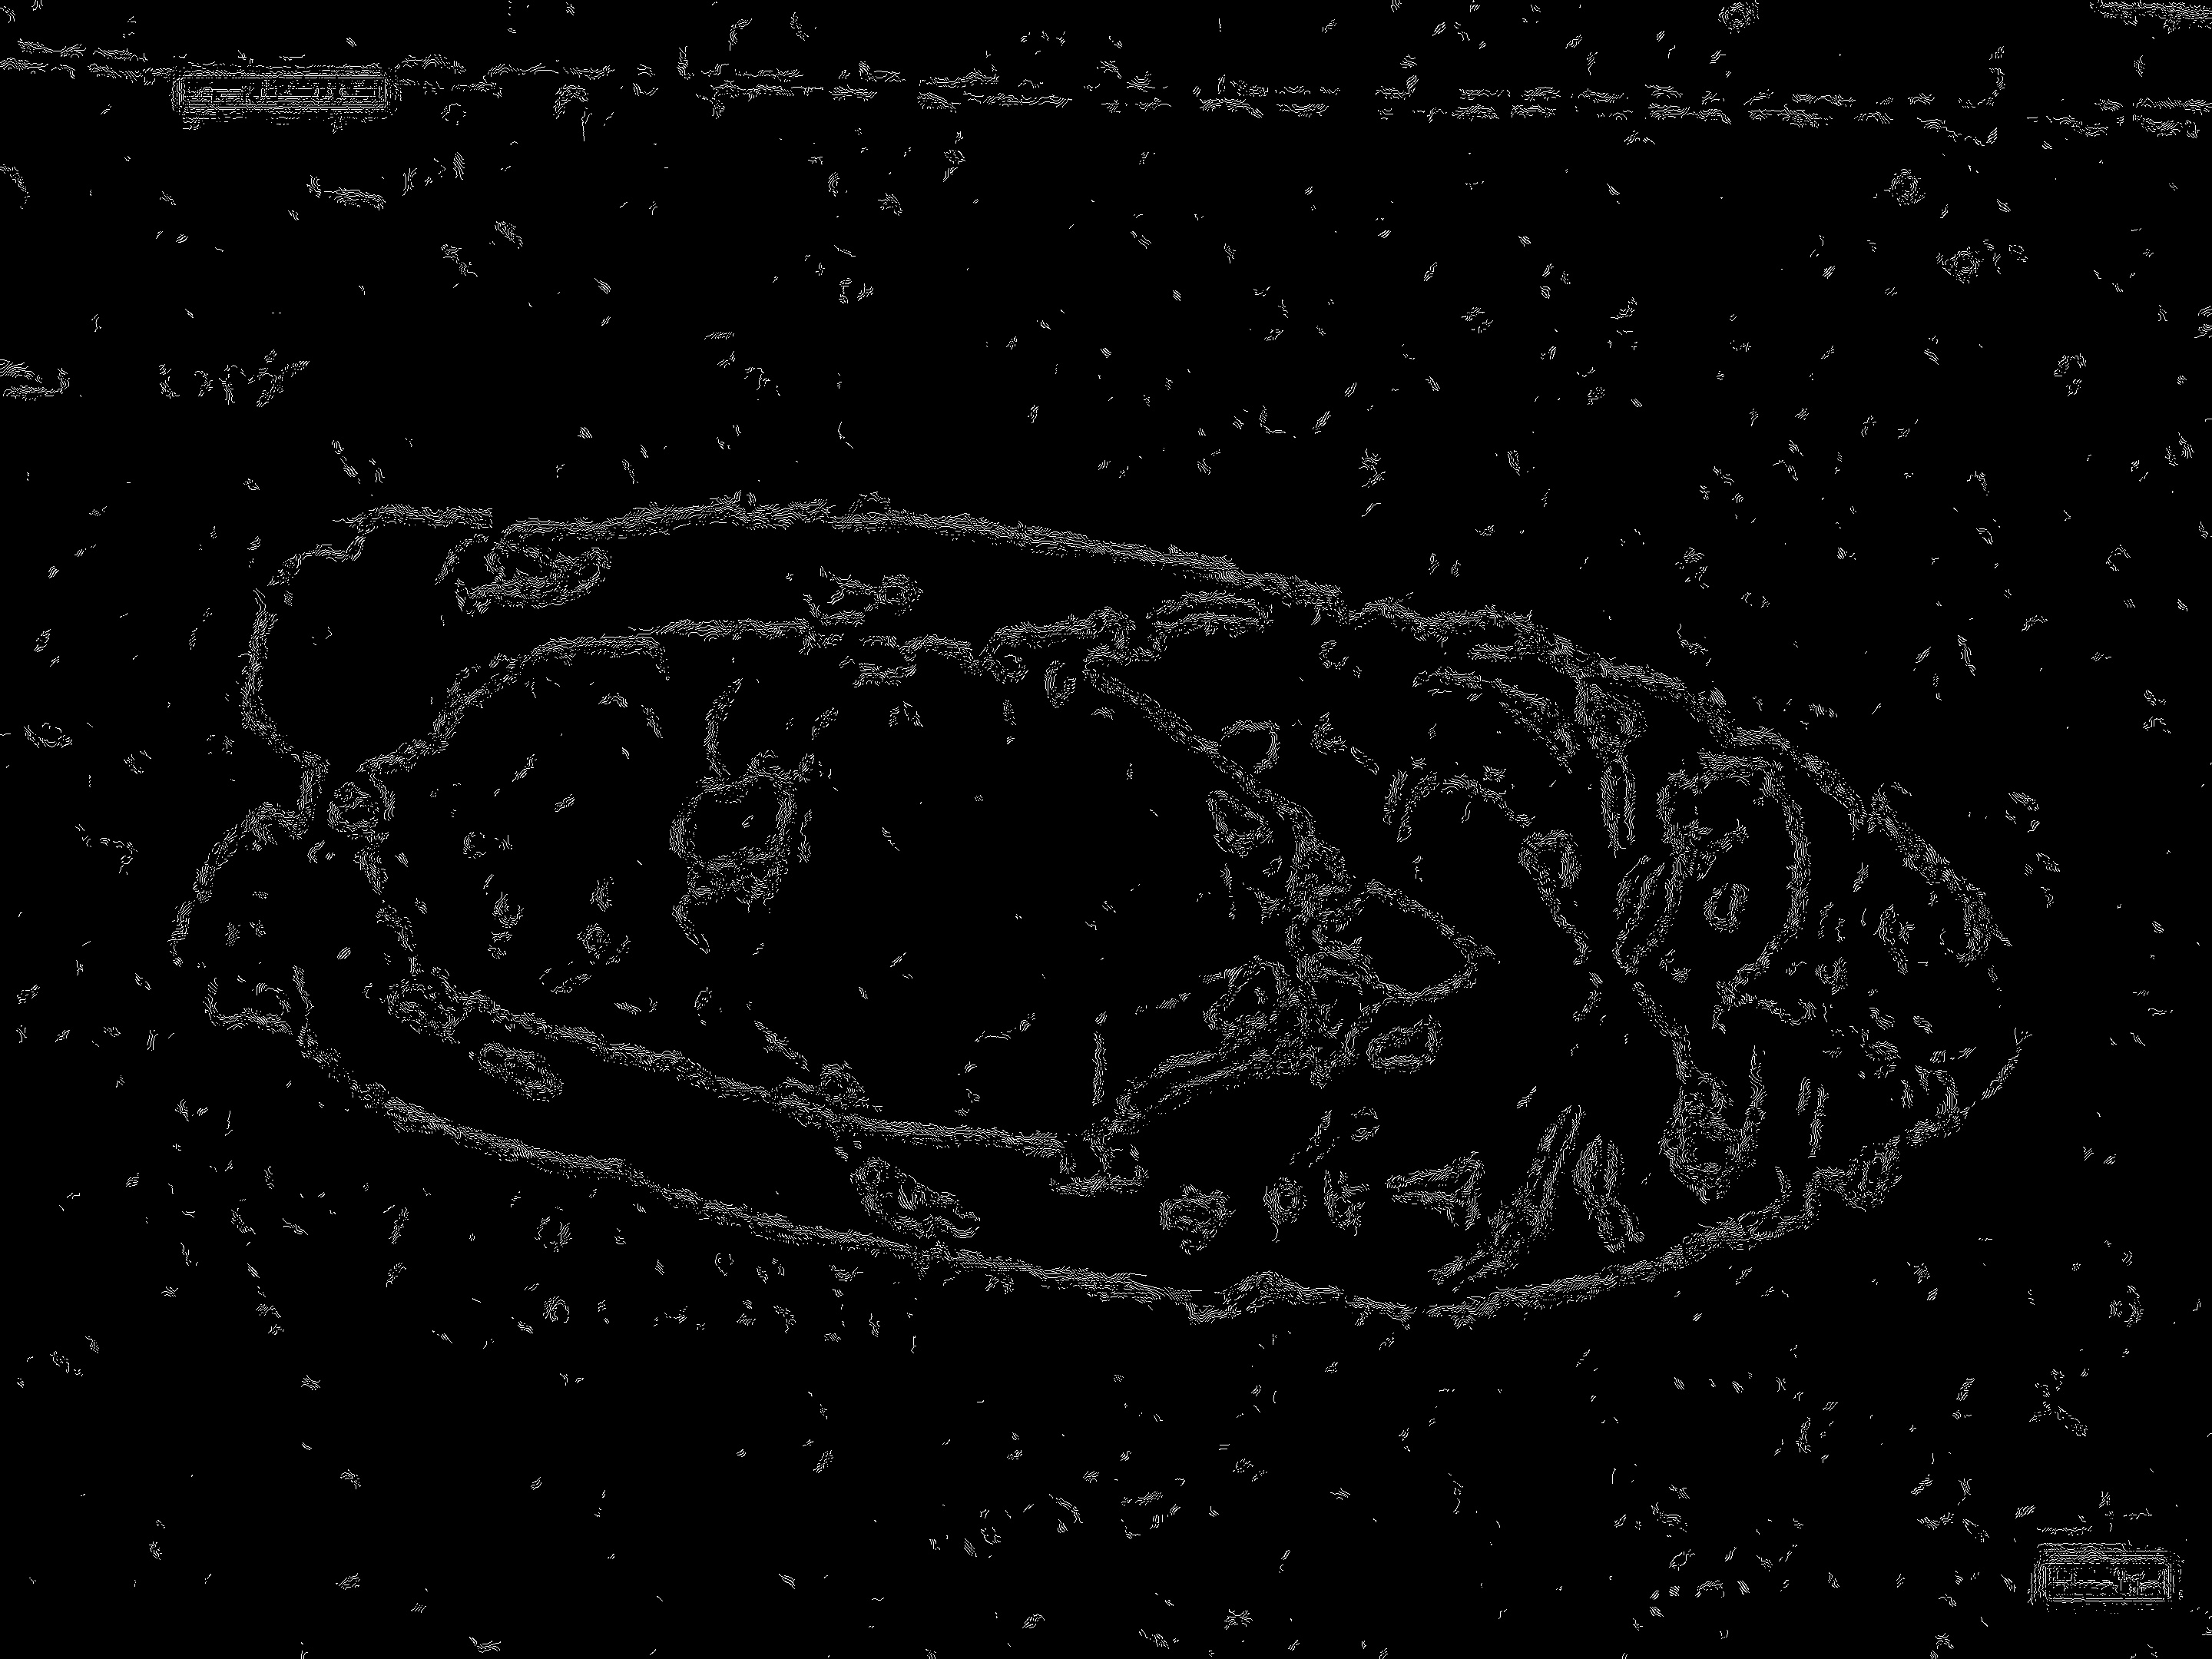
\includegraphics[width=\textwidth]{./fig/gausssian/canny61+4.jpg}
        \caption{canny 4 10}
        \label{fig:canny4_10}
    \end{minipage}
    \begin{minipage}{0.32\textwidth}
        \centering
        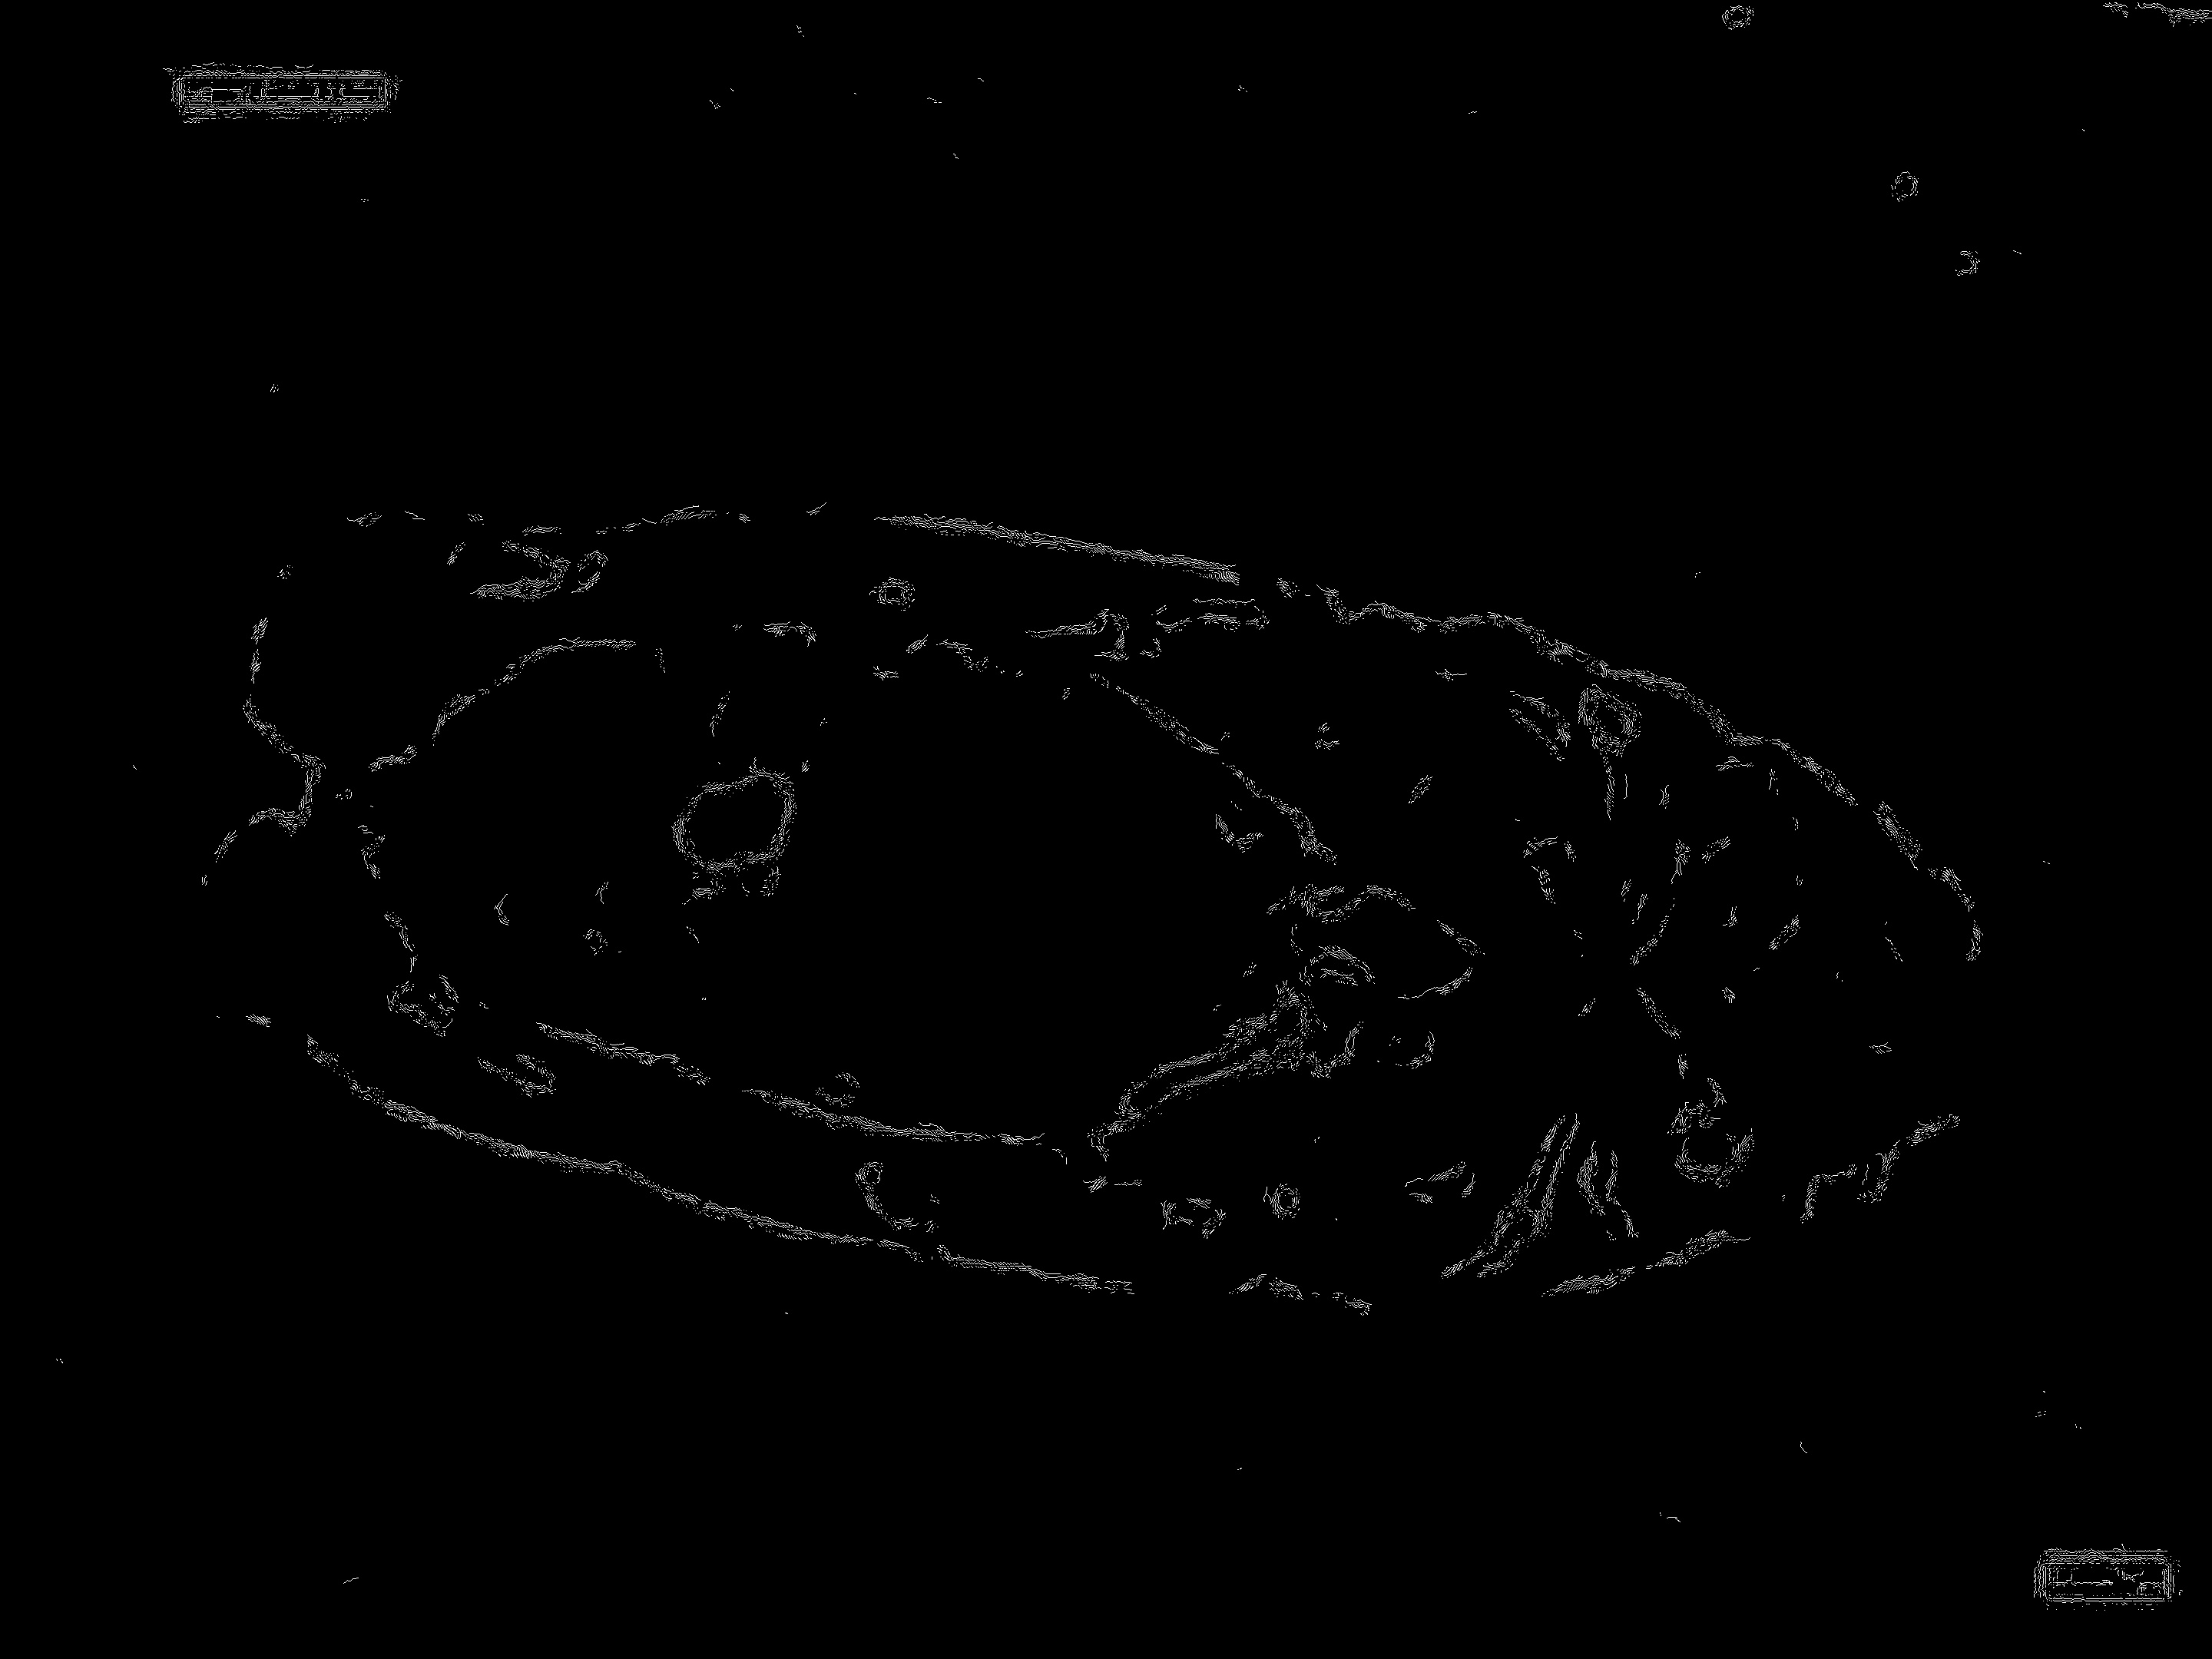
\includegraphics[width=\textwidth]{./fig/gausssian/canny61+6.jpg}
        \caption{canny 6 15}
        \label{fig:canny6_15}
    \end{minipage}
\end{figure}


在三张canny算法的结果中,可见\autoref{fig:canny4_10}的效果最好,其能在保证边缘细节得到大部分保留的情况下,去除了大部分的噪声。因此我们选择canny算法的阈值为4 10。

\textbf{总结}

对比sobel, laplacian和canny算法的结果,sobel算法的效果一般,对于底噪不是能很好的去除,边缘检测效果还算显著。laplacian算法最差,边缘甚至已经不可见,这可能是因为该算法对噪声最敏感。canny算法的效果最好,能够在保证边缘细节的情况下,去除大部分的噪声。因此我们选择canny算法作为图像预处理的方法。

\FloatBarrier


\subsubsection{阈值分割}

考虑到生物组织样本的主体是黄色,石蜡是白色,我们可以通过设置一个阈值,将图像中的白色部分分割出来,那么剩下的就是生物组织部分。在这里使用python的opencv库中进行操作。首先将图像进行对比度增强,增加饱和度,更好的凸显出生物组织的颜色(\autoref{fig:enhanced_image})。之后读取图像的每个像素点,将黄色周围半径15左右的像素点进行保留(约为图像宽的百分之一),其他的色块进行去除。(如\autoref{fig:yellowpic})。

\begin{figure}[H]
    \centering
    \begin{minipage}{0.4\textwidth}
        \centering
        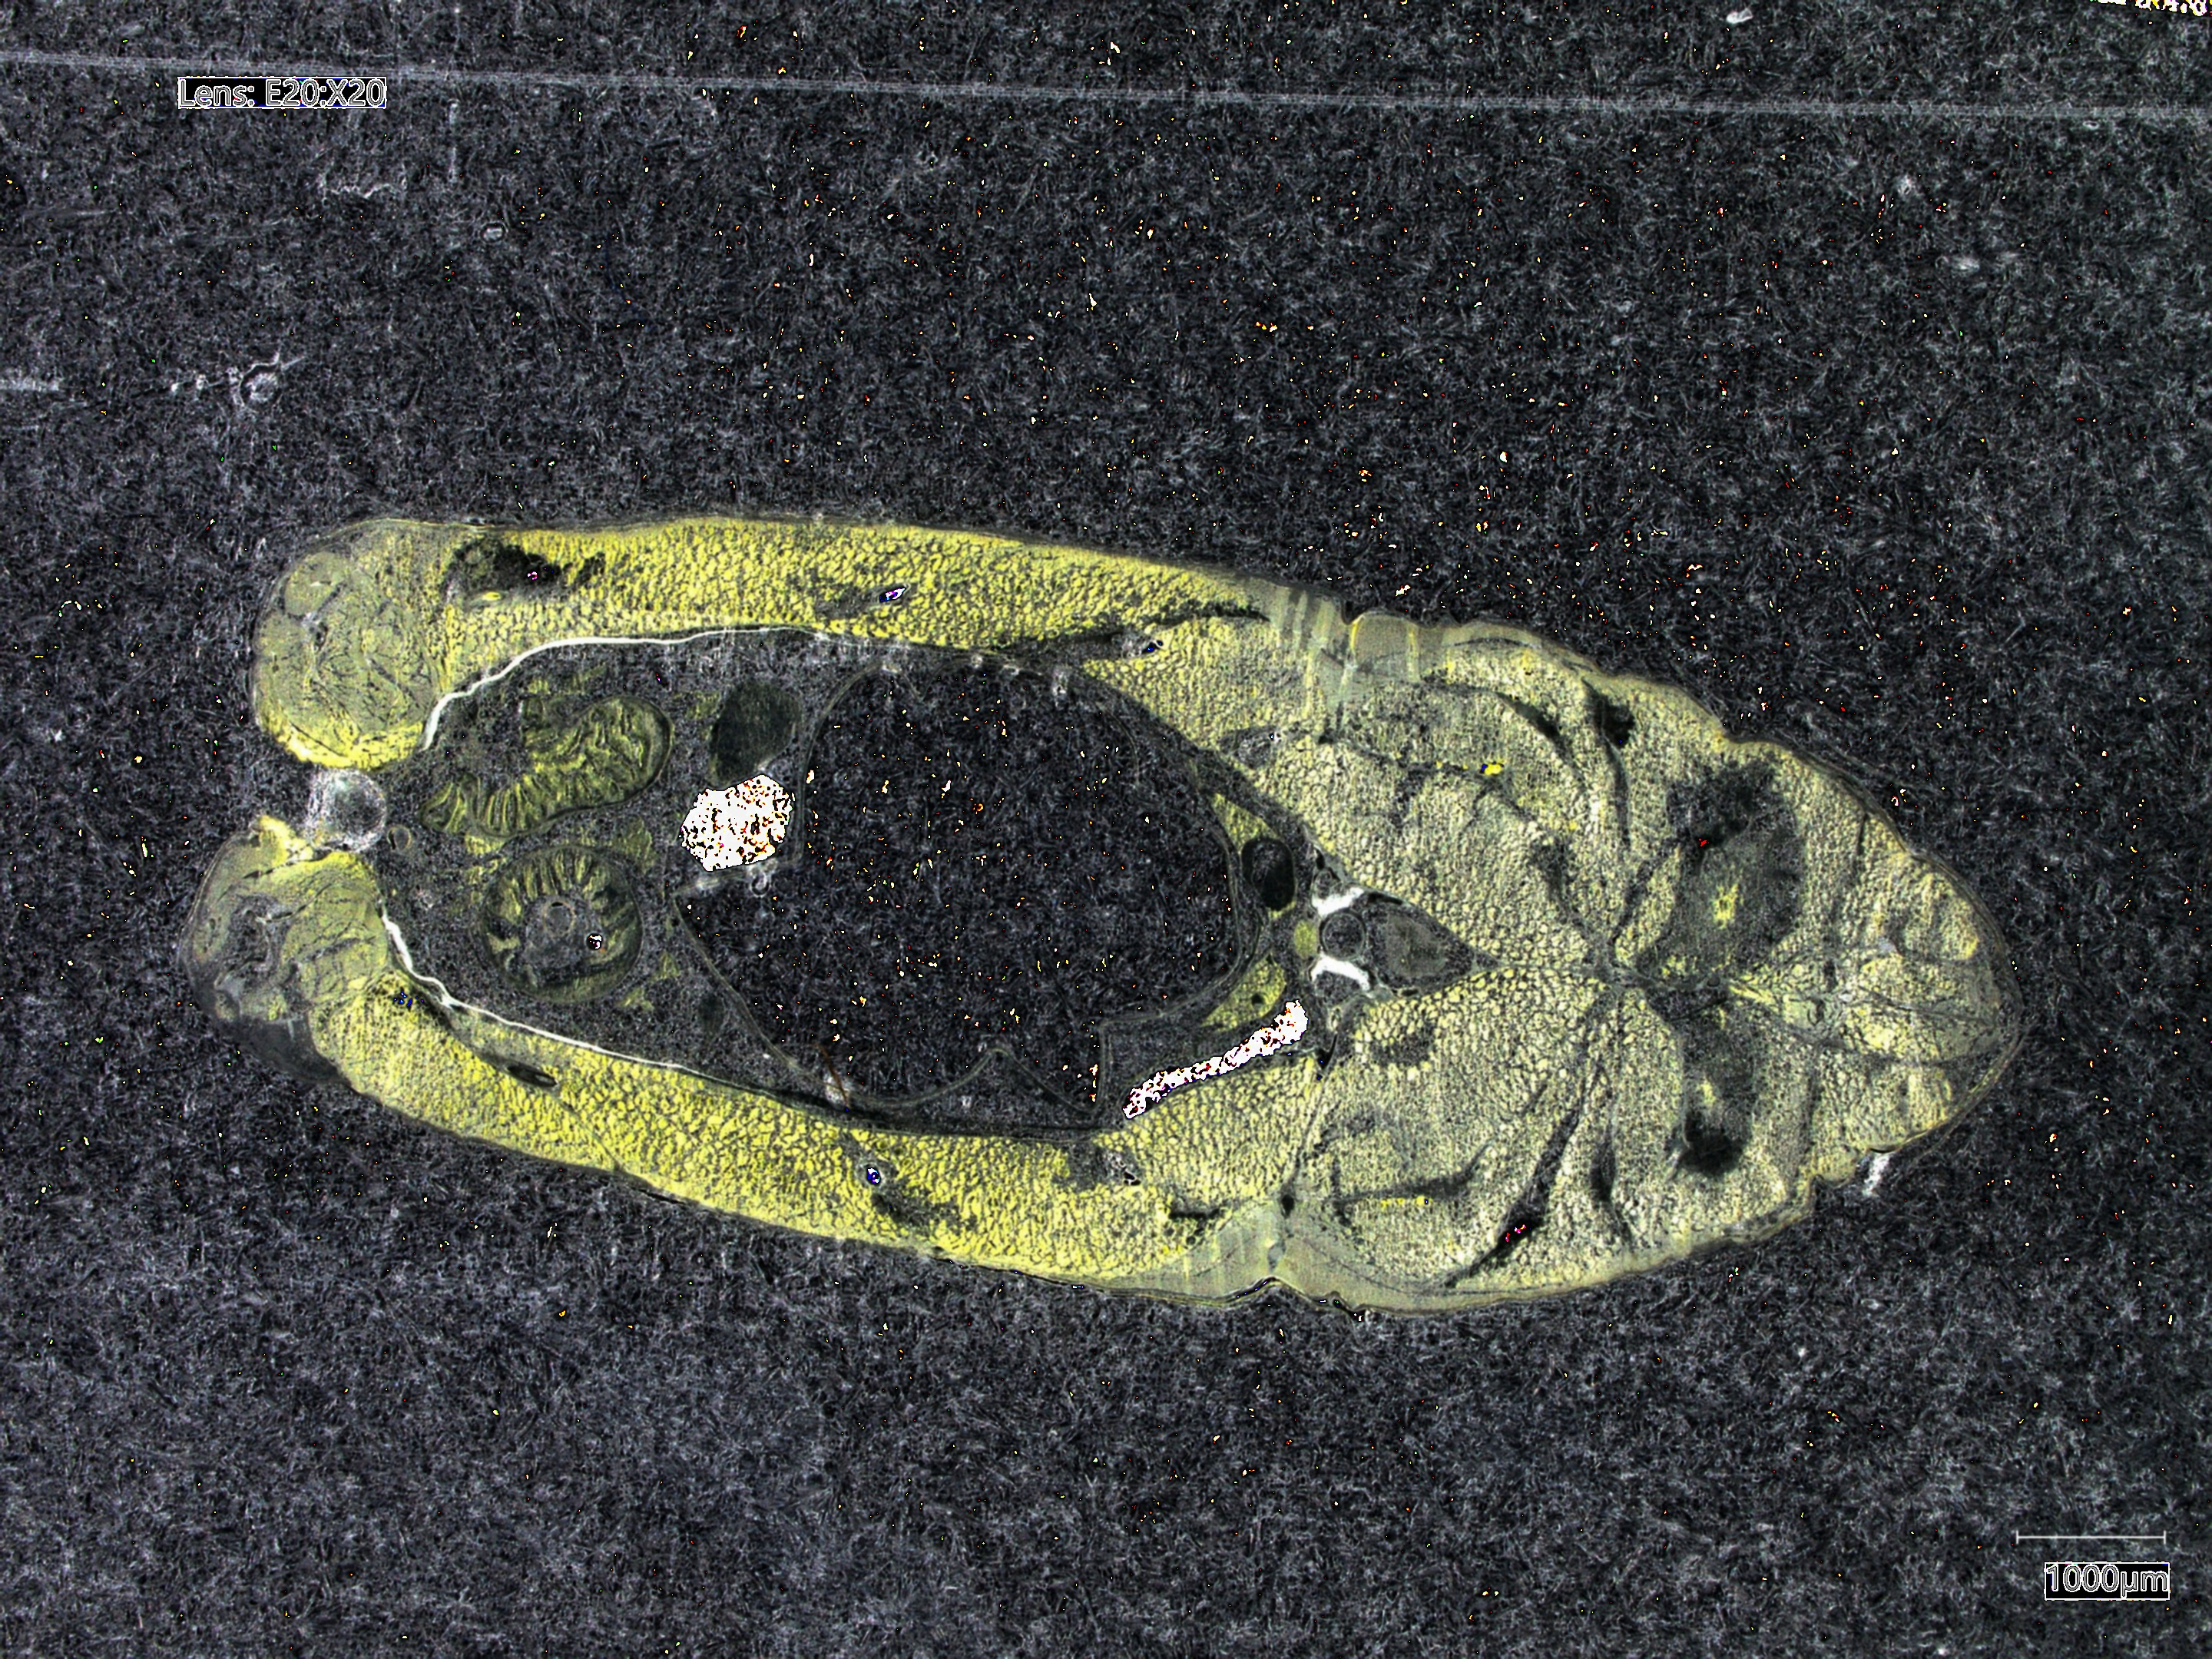
\includegraphics[width=\textwidth]{./fig/threshold/enhanced_image.jpg}
        \caption{enhanced image}
        \label{fig:enhanced_image}
    \end{minipage}
    \begin{minipage}{0.4\textwidth}
        \centering
        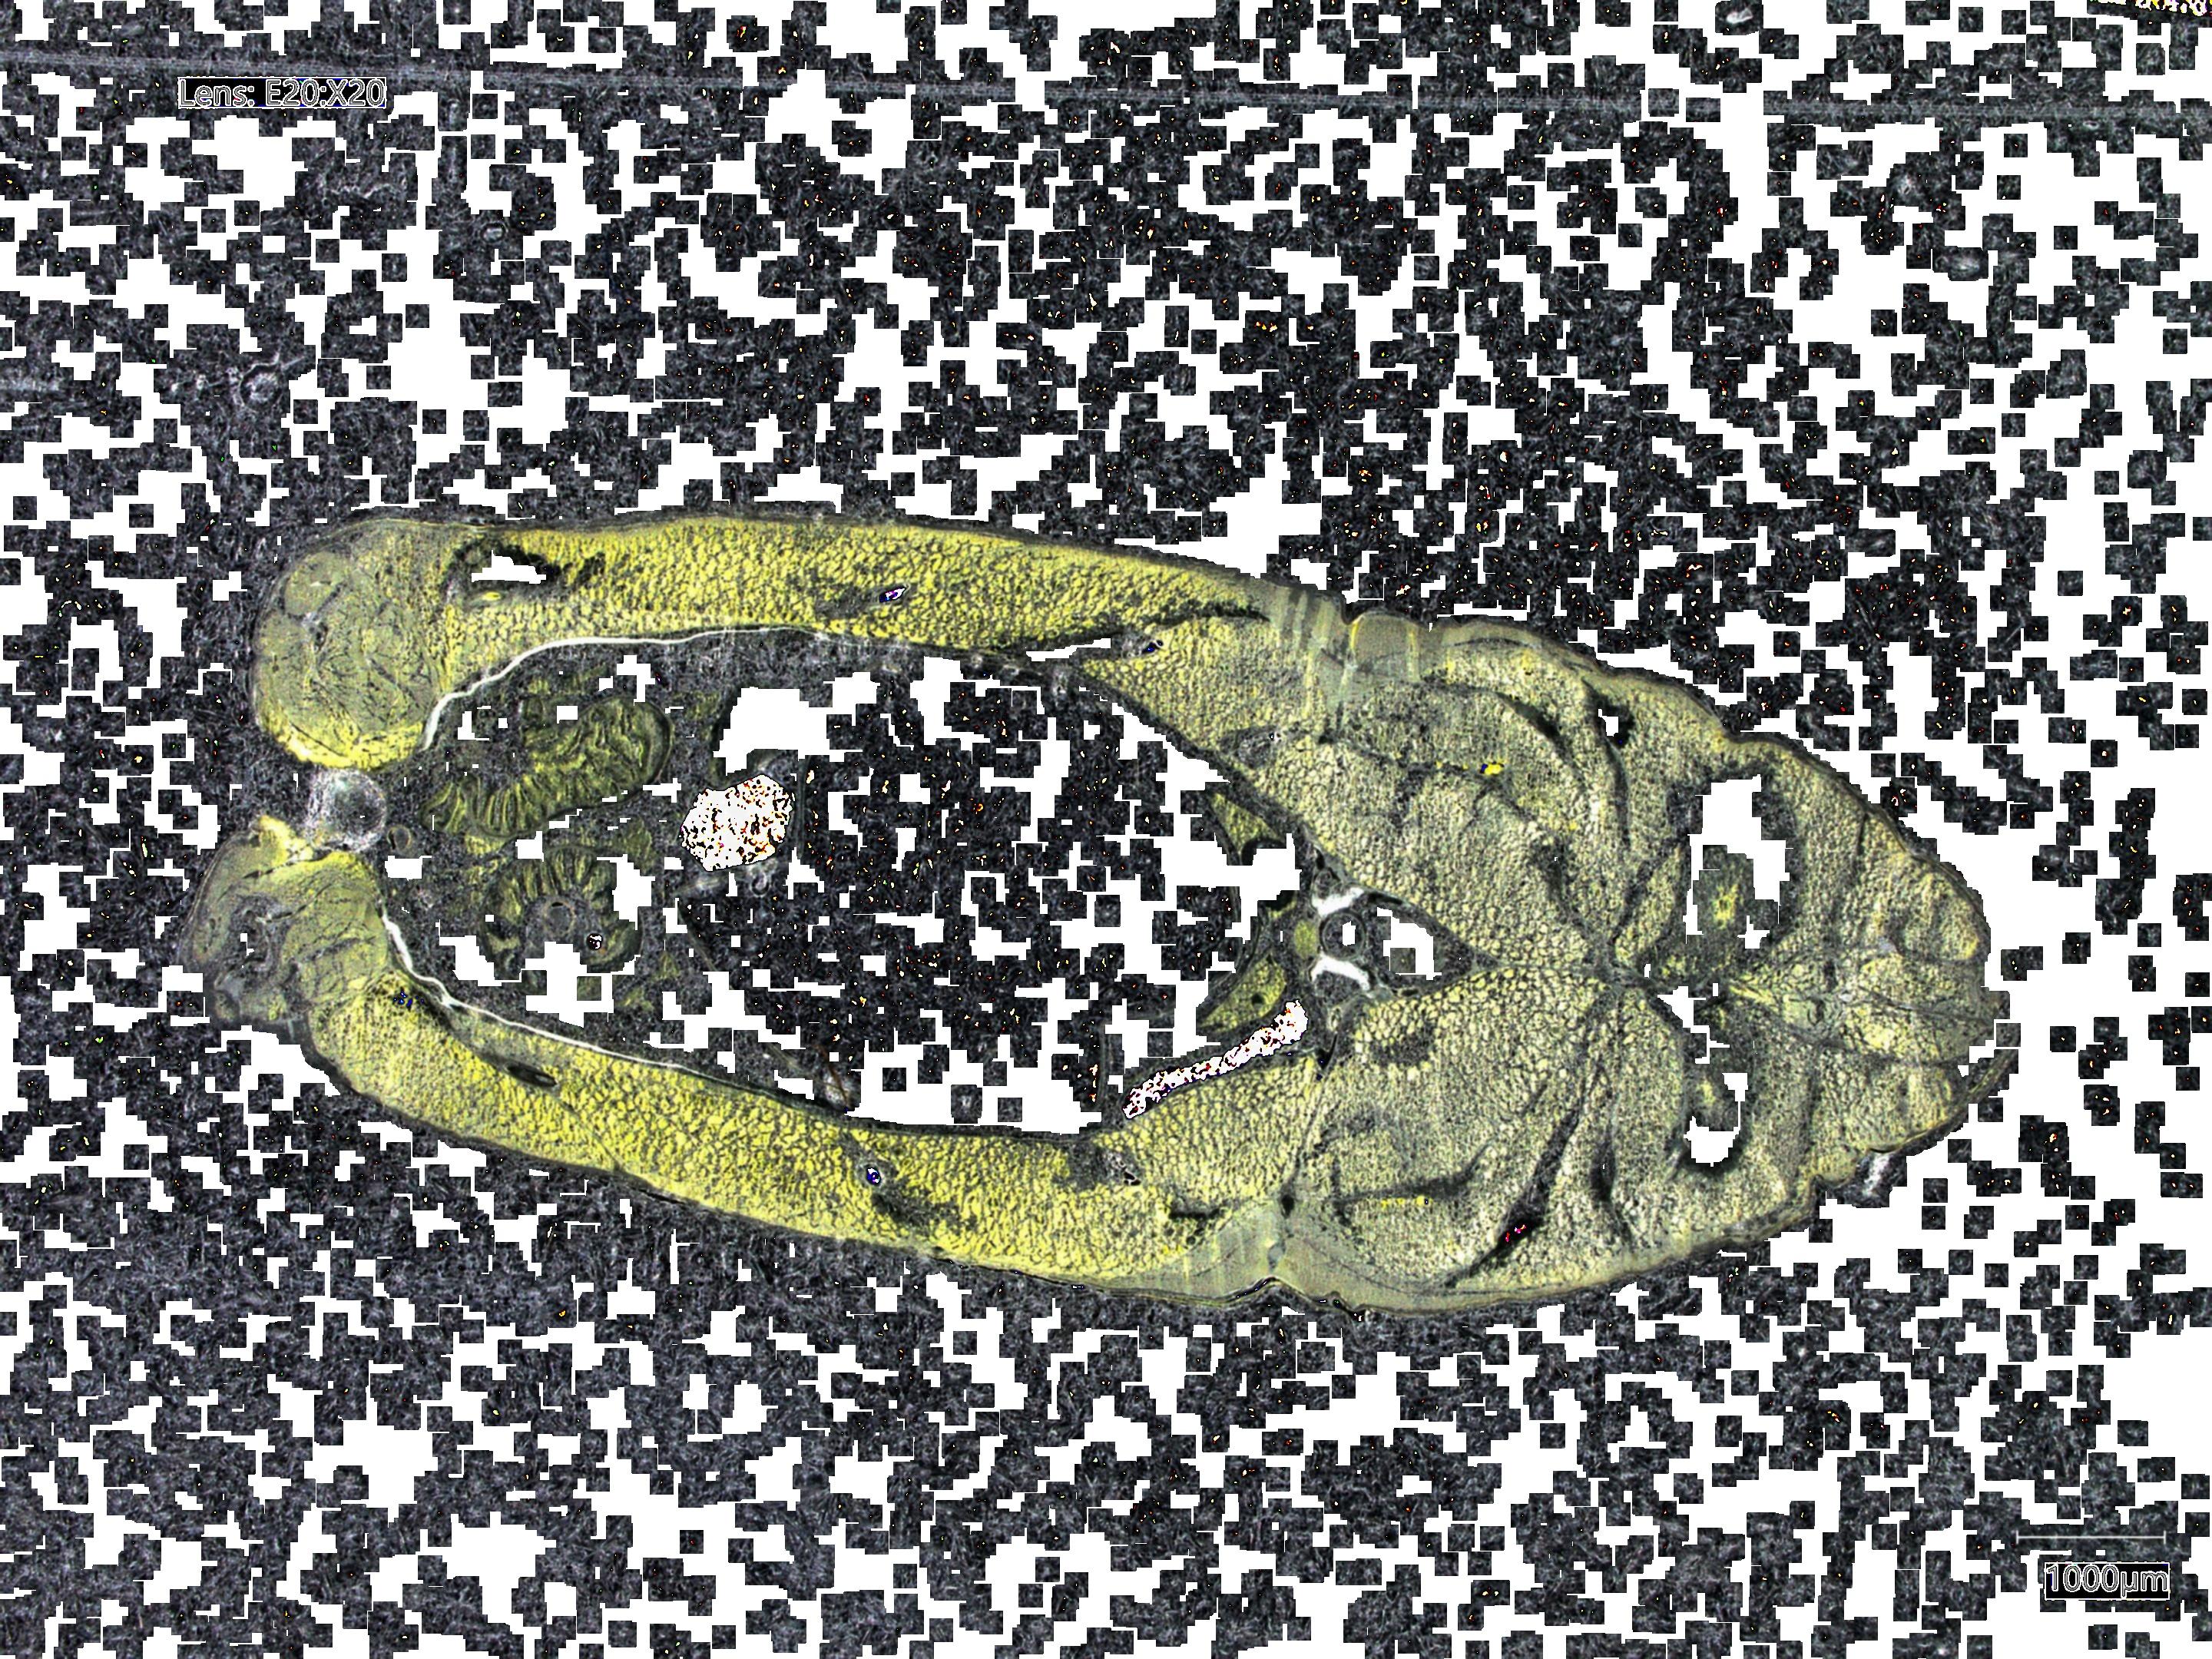
\includegraphics[width=\textwidth]{./fig/threshold/yellowpic.jpg}
        \caption{yellow picture}
        \label{fig:yellowpic}
    \end{minipage}
\end{figure}

但是观察发现,这种方法对于生物组织和石蜡的分割效果并不好,因为生物组织在切片过程中会掉落碎片组织,出现在标本各处,进而影响黄色像素点的识别。此时还需要进一步的处理,去除黑色色块。此时只需要将黑色色块进行掩码反转,使其变为白色即可。结果如图\autoref{fig:mask}所示。

\begin{figure}
    \centering
    \begin{minipage}{0.4\textwidth}
        \centering
        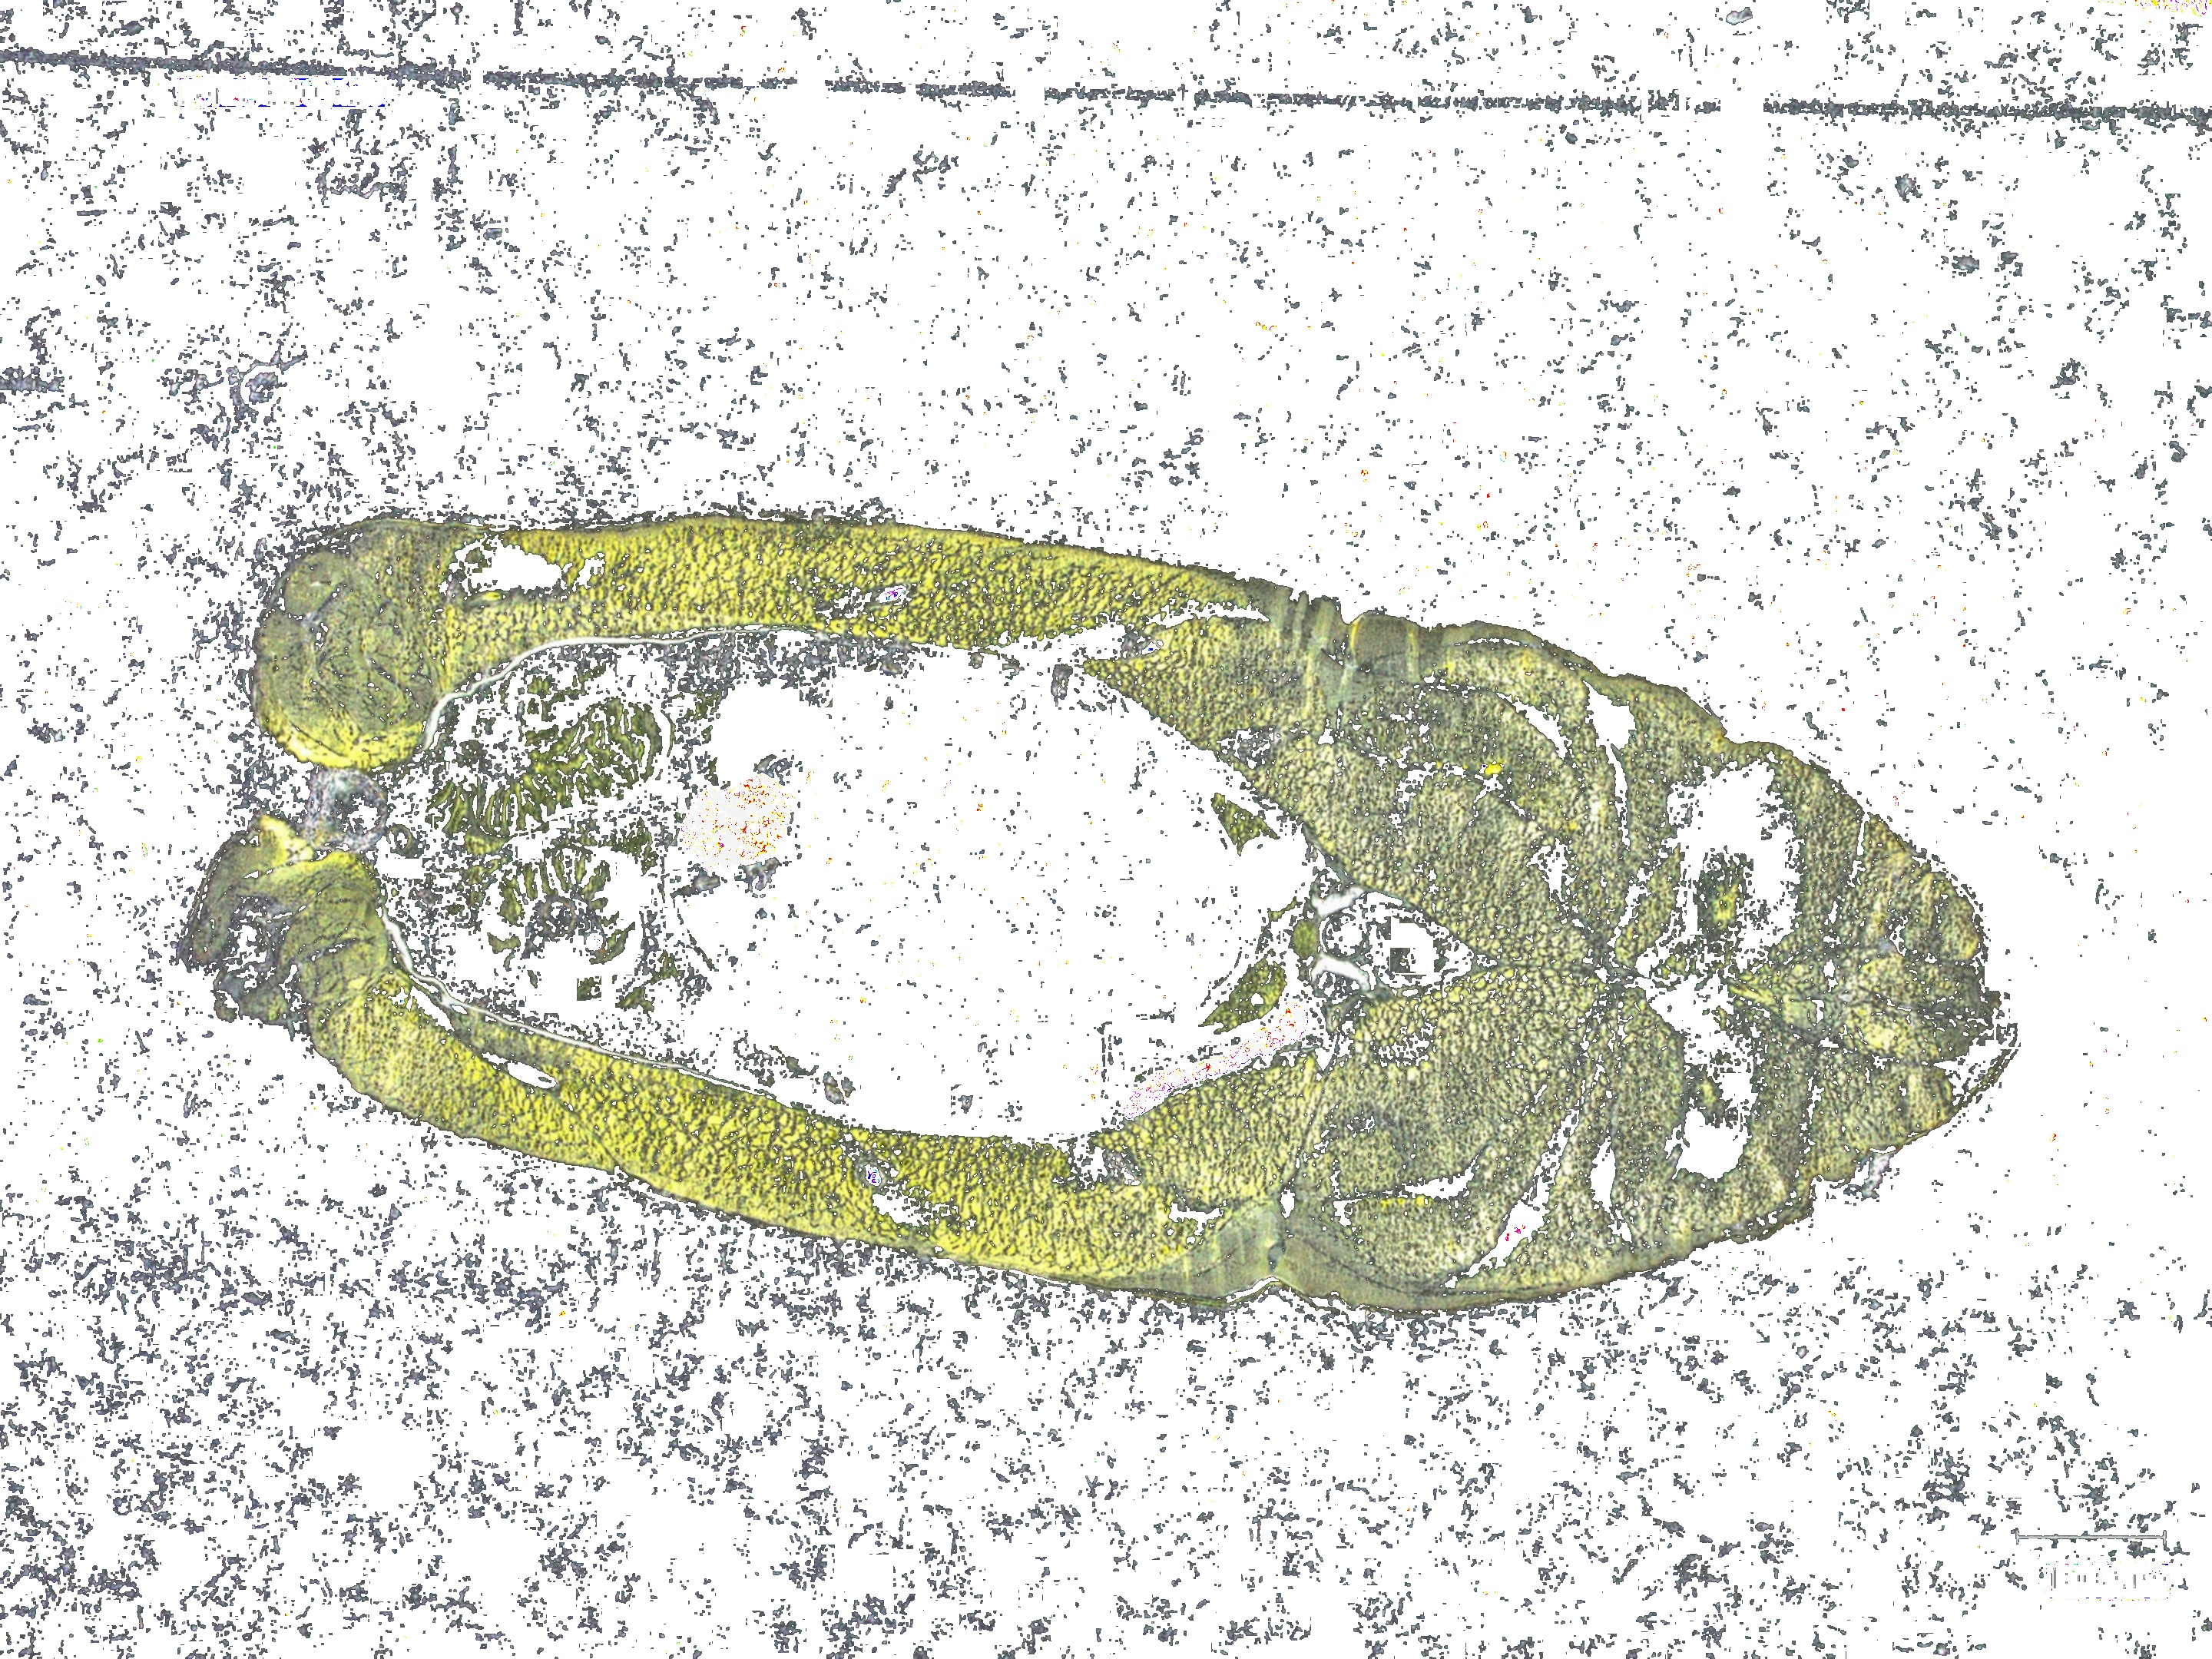
\includegraphics[width=\textwidth]{./fig/threshold/final.jpg}
        \caption{final}
        \label{fig:mask}
    \end{minipage}
    \begin{minipage}{0.4\textwidth}
        \centering
        \includegraphics[width=\textwidth]{./fig/threshold/fingerprint.jpg}
        \caption{fingerprint}
        \label{fig:fingerprint}
    \end{minipage}
\end{figure}

\subsubsection{另一种阈值分割方法-指纹算法}
在进行文献综述的时候,发现有一篇论文是基于otsu算法改进的分割方法用于进行指纹分割。考虑到切片样本和指纹都属于生物组织,因此我们尝试使用论文中提到的算法进行分割。结果如图\autoref{fig:fingerprint}所示。

\subsubsection{小结}
根据上文提到的图像预处理方法,我们可以看到,边缘检测和阈值分割的效果都不错,都能够很好的突出生物组织的特征,去除石蜡的干扰。对此我们可以设置三组数据集,分别是经过边缘检测后的图像,经过阈值分割后的图像和经过指纹算法分割后的图像。这三组数据集将作为我们的训练集,用于下一节的模型训练。

\FloatBarrier



\subsection{模型2:预处理图像+简单的cnn网络}

在这里基础模型选用在上一节模型1中表现最好的模型1c。在这里我们将模型1c的输入改为经过预处理后的图像,即经过\textbf{边缘检测后,阈值分割和指纹算法分割后的图像}。在这里模型的架构不变,只是输入的数据发生了变化。

所有的模型2采用和模型1c同样的架构构成,分别由三个包含32个特征图,卷积核为3*3的卷积层和最大池化层,一个包含256个神经元的全连接层组成。模型2a的输入为经过\textbf{canny边缘检测}后的图像。
模型2b采输入为经过\textbf{阈值分割}后的图像。
模型2c输入为经过\textbf{指纹算法分割}后的图像。

结果如下:
\begin{figure}
    \centering
    \begin{minipage}{0.49\textwidth}
        \centering
        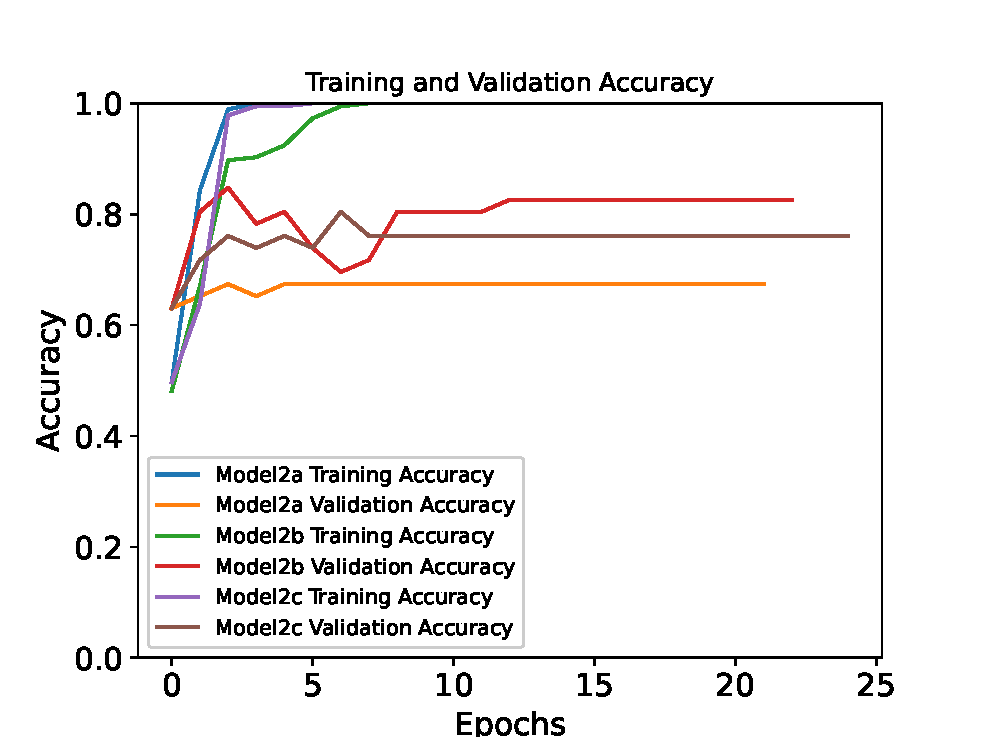
\includegraphics[width=\textwidth]{./fig/model2/accuracy22.eps}
        \caption{Model 2 accuracy}
        \label{fig:model22_acc}
    \end{minipage}
    \begin{minipage}{0.49\textwidth}
        \centering
        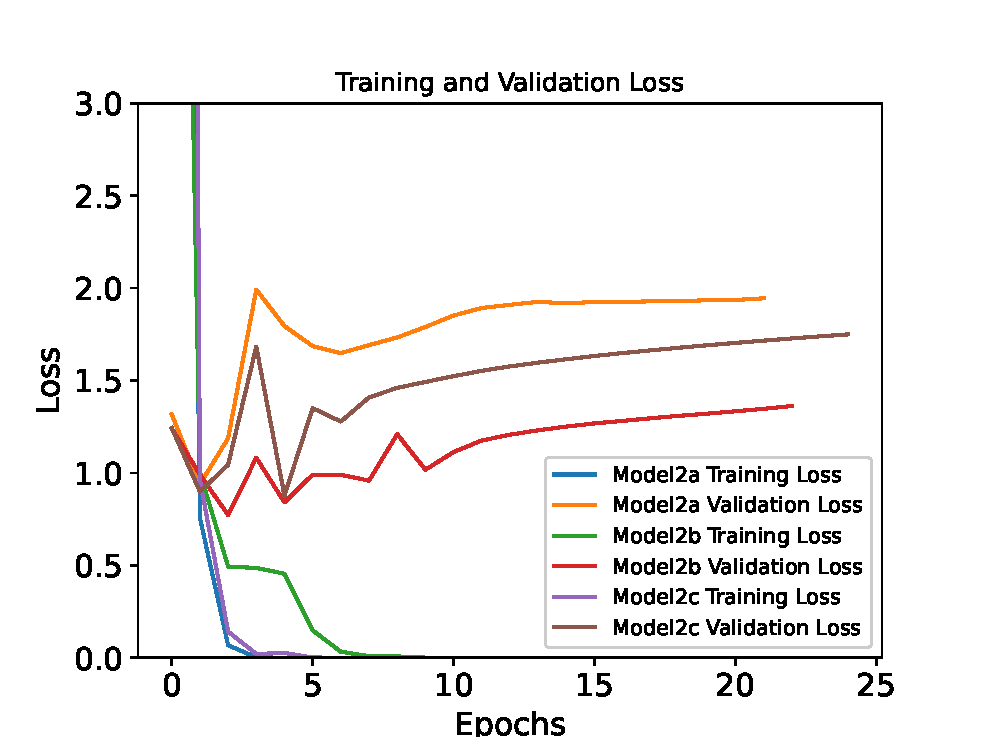
\includegraphics[width=\textwidth]{./fig/model2/loss22.eps}
        \caption{Model 2 loss}
        \label{fig:model22_loss}
    \end{minipage}
\end{figure}


\subsubsection{小结}
在图中,对比了模型2a、2b和2c的训练和验证准确度以及损失的变化情况。模型2a和模型2c的训练和验证准确度在经过约8个训练周期后开始趋于稳定,其中训练准确度接近于100\%,而验证准确度稳定在65\%和75\%左右。尽管准确度较高,两者的验证损失仍旧较高,都在1以上。这可能指示了模型对训练数据过拟合,而对未见数据的泛化能力有限。

对于模型2b,其在约10个训练周期后开始收敛,与模型2a和2c相比,模型2b拥有最高的的验证准确度,约为82\%左右,但是其损失显著低于模型2a和2c,在1-1.2波动。这表明模型2b在泛化到验证集上时的性能更优,损失更低,反映了模型更好的适应性和鲁棒性。

可能原因是模型2a和2c可能处理的是灰度图像,而模型2b处理的是彩色图像。彩色图像包含的RGB通道信息可以提供更丰富的特征,从而可能增强了模型的特征提取和泛化能力。然而,即使彩色图像提供了额外信息,前处理步骤,尤其是模型2b的阈值分割,可能会导致重要细节的丢失,这反过来可能会影响到模型在特定图像上的表现。这种情况下,模型的预处理步骤需要仔细检查,以确保不会因过于激进的图像简化而丢失关键信息。

一个丢失关键信息的例子如下所示:

\begin{figure}
    \centering
    \begin{minipage}{0.45\textwidth}
        \centering
        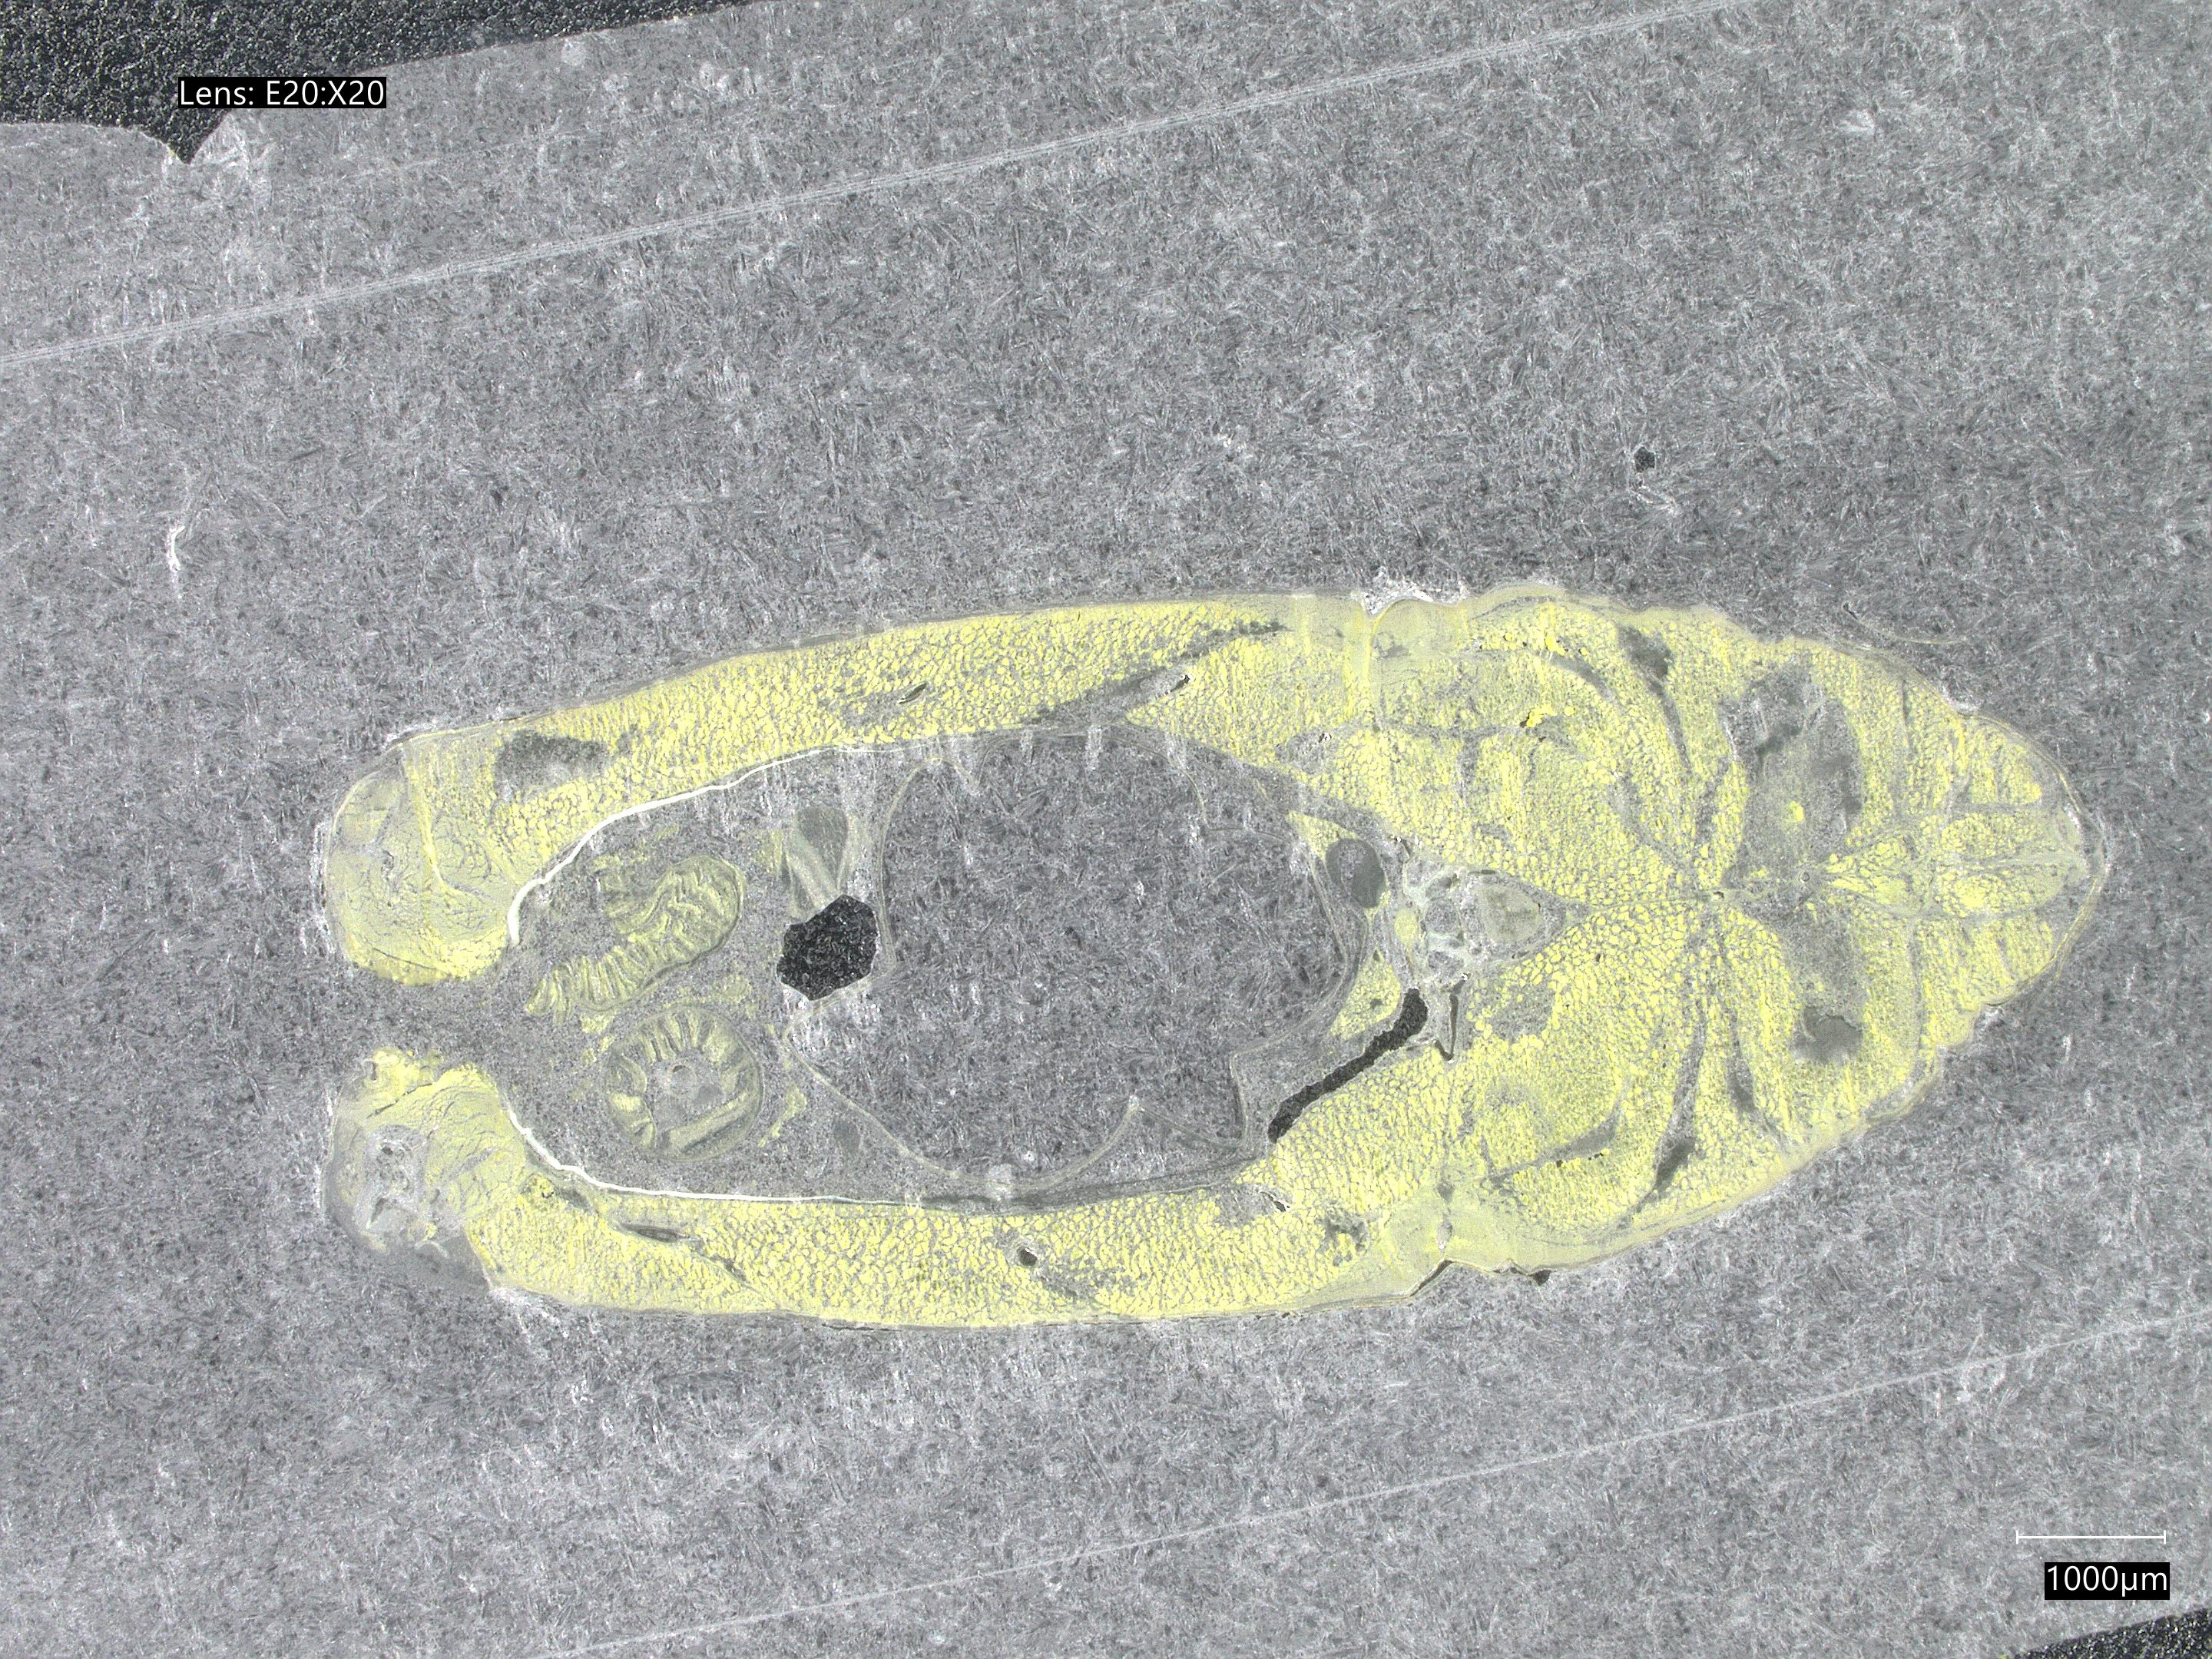
\includegraphics[width=\textwidth]{./fig/model2/origin20240205_161427.jpg}
        \caption{origin}
        \label{fig:origin}
    \end{minipage}
    \begin{minipage}{0.45\textwidth}
        \centering
        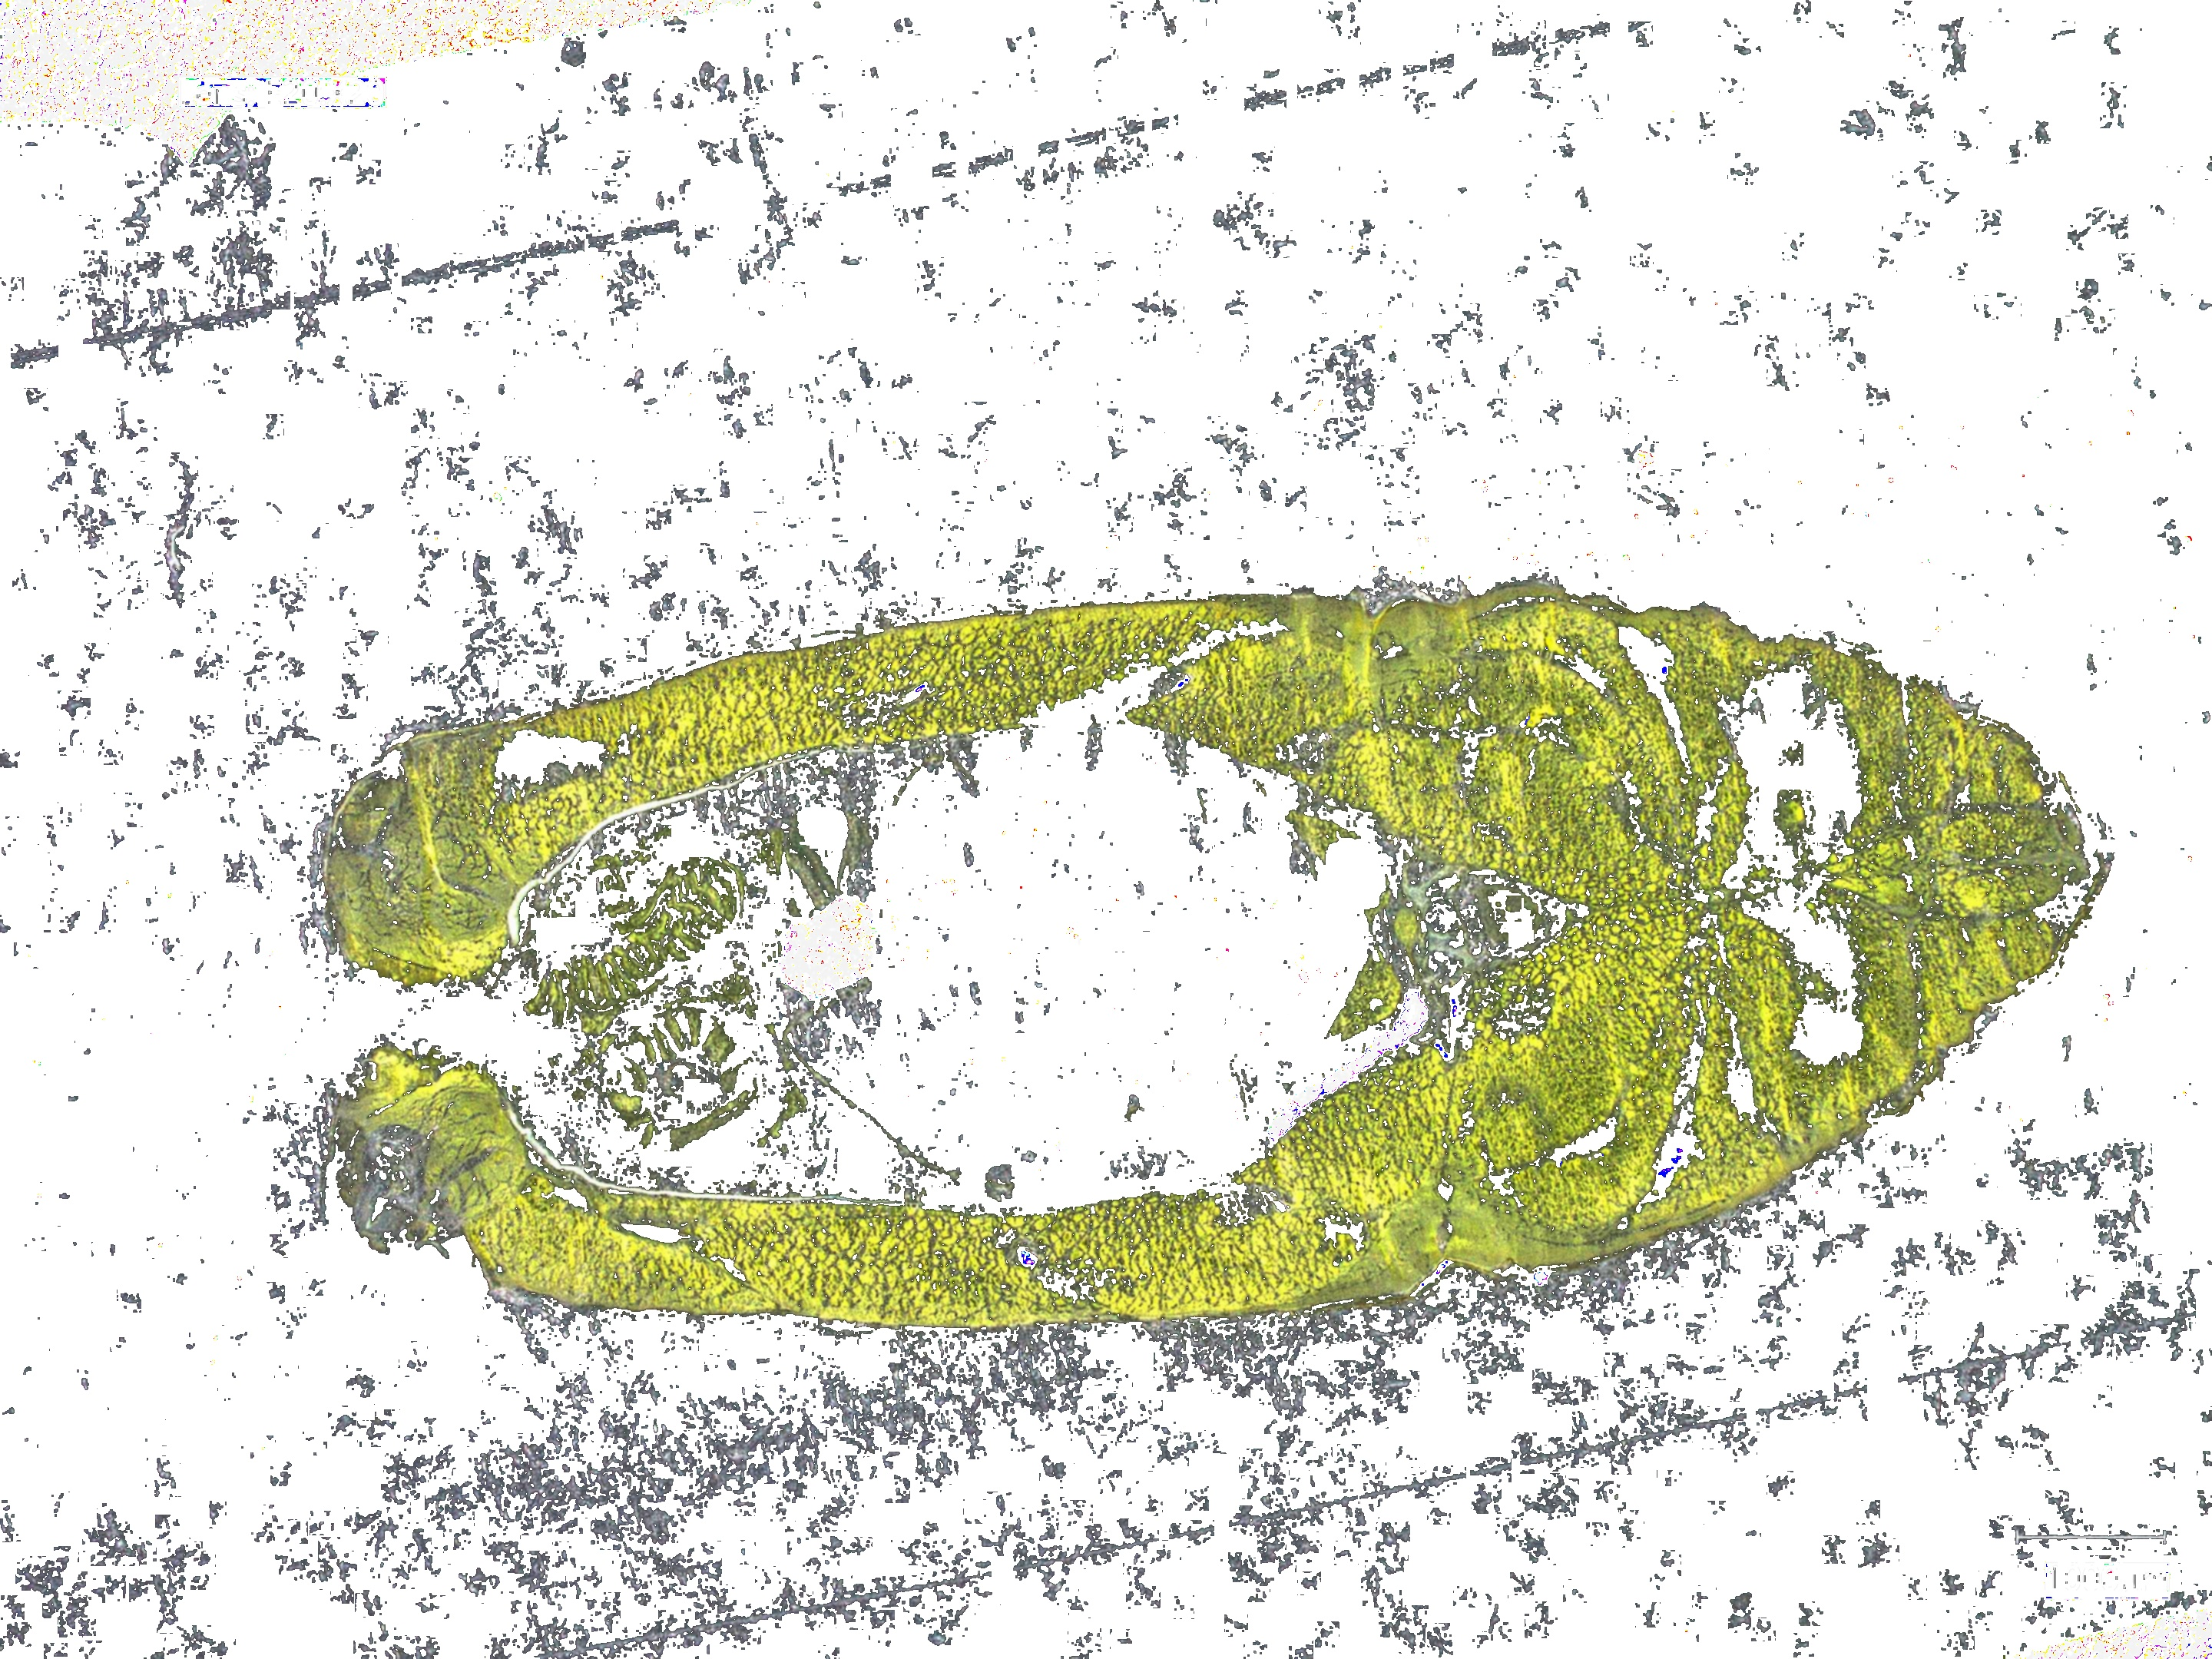
\includegraphics[width=\textwidth]{./fig/model2/yellow20240205_161427.jpg}
        \caption{yellow}
        \label{fig:yellow}
    \end{minipage}
\end{figure}

\autoref{fig:yellow}是模型2b训练集(经过黄色阈值分割后的图像)中的一张图片,对比原图(\autoref{fig:origin})可以观察发现,原本切片中能够被接受的水平褶皱瑕疵被阈值分割算法显著增强了,这有极有可能会影响模型的训练效果,即模型会在一定程度上与horizental line混淆。

由此可以看出,对于图像预处理,其实并不能显著的提高模型的训练效果,反而可能会因为过于激进的预处理而丢失关键信息,导致模型的训练效果下降。在后面将会尝试使用迁移学习的方法,使用预训练好的大规模深度学习模型,将其迁移到我们的数据集上,以提高模型的训练效果。

\FloatBarrier

\subsection{模型3:原始图像+迁移学习}

现在我们已经尝试过了简单的cnn网络,以及对图像进行预处理后的cnn网络。既然训练结果不是很理想,那我们为什么不去尝试更大更深的模型? 在这一节,我们尝试使用迁移学习的方法,使用预训练好的大规模深度学习模型,将其迁移到我们的数据集上,以提高模型的训练效果。

正如在第三节methodology里提到的,在这里将使用VGG16,VGG19和InceptionV3三个模型进行迁移学习。这三个模型都是在ImageNet数据集上训练好的模型,具有已经训练好的权重。

在这里为了避免迁移学习过拟合,不仅使用了原有的早停法,还限制了模型的学习率为1e-5(对于inceptionV3模型,学习率为1e-4)。

model3a是使用VGG16模型进行迁移学习的模型。model3b是使用VGG19模型进行迁移学习的模型,VGG19和VGG16相比只是在中间增加了3个额外的卷积层,其他则与VGG16相同。model3c是使用InceptionV3模型进行迁移学习的模型,其中InceptionV3是一个相对于VGG16和VGG19更加复杂的模型,其在训练过程中引入了Inception模块,能够更好的提取图像的特征。

在这里统一将模型的输入调整为224*224,因为VGG16和VGG19模型在预训练时的输入层是224*224的图像,而InceptionV3的默认值为299*299的图像。

并且,在基础模型后面还需要添加一个全局平均池化层,一个全连接层。全局平均池化层的作用是将每个特征图减小到一个单一的数值,全连接层的作用是将全局平均池化层的输出转换为我们需要的输出,其输出节点的个数则和分类的数量相等。

\begin{figure}[H]
    \centering
    \begin{minipage}{0.49\textwidth}
        \centering
        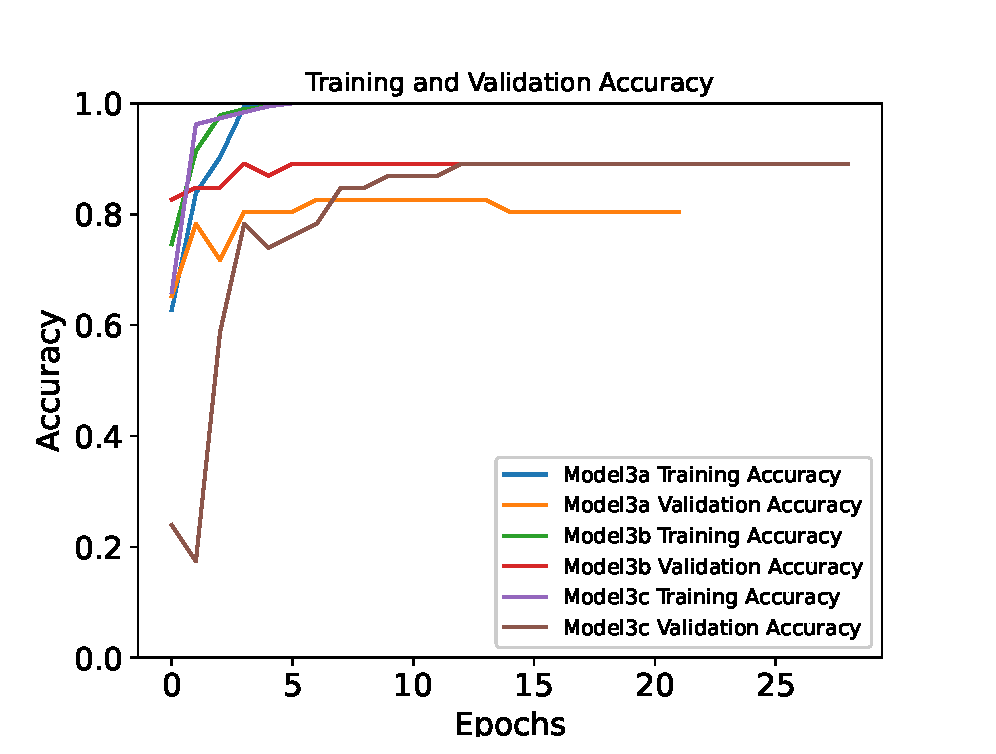
\includegraphics[width=\textwidth]{./fig/model3/accuracy33.eps}
        \caption{Model 3 accuracy}
        \label{fig:model33_acc}
    \end{minipage}
    \begin{minipage}{0.49\textwidth}
        \centering
        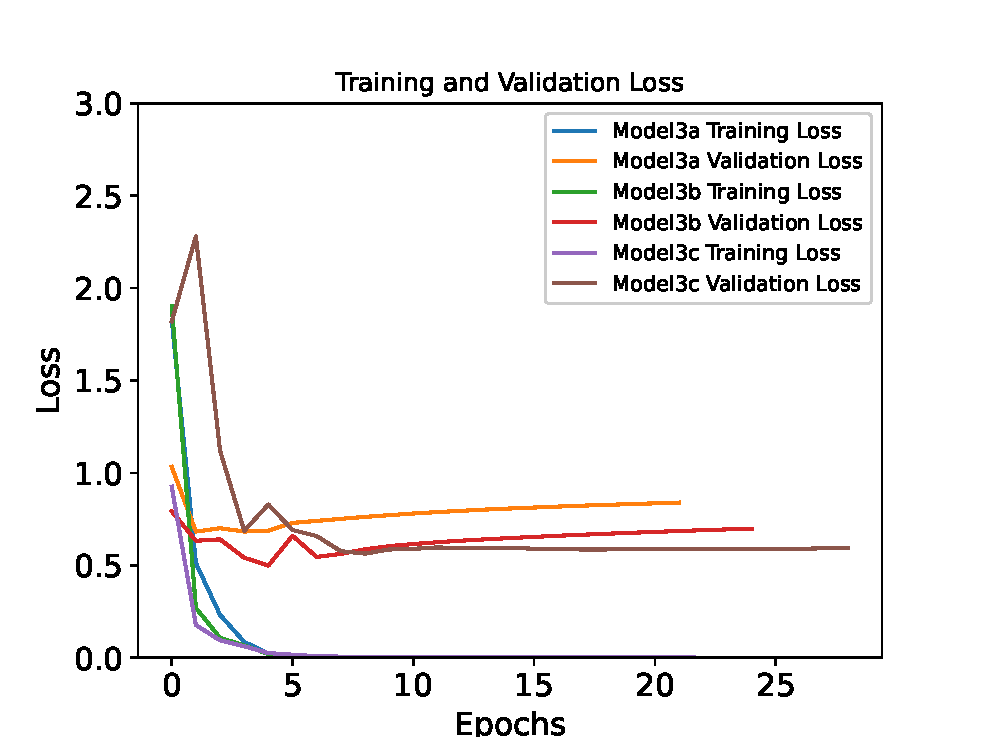
\includegraphics[width=\textwidth]{./fig/model3/loss33.eps}
        \caption{Model 3 loss}
        \label{fig:model33_loss}
    \end{minipage}
\end{figure}

对比三个模型,可以观察得到model3b和model3c的验证集的准确度显著高于model3a,约为90\%左右。观察损失图,可以得出model3c在这三个模型中验证集的损失是最低的,model3b次之,model3a表现最差。这可能是因为InceptionV3模型的复杂度更高,能够更好的提取图像的特征。而VGG16和VGG19模型相对于InceptionV3模型而言,更加简单,可能在提取图像特征上存在一定的局限性。此外,model3b性能显著高于model3a可以说明,VGG19模型相对于VGG16模型而言,多出的三个卷积层能够更好的提取图像的特征。符合模型的复杂度越高,其训练效果越好的规律。

\subsubsection{小结}

对比VGG16,VGG19和InceptionV3三个模型,可以发现InceptionV3的训练效果最好,其训练准确度和验证准确度收敛于1和0.9左右,损失收敛于0.6左右。这说明InceptionV3模型的训练效果最好,其泛化能力最强。

\subsection{模型选择总结}

当比较模型系列——模型1,模型2和模型3时,显然模型3的表现最好,特别是模型3c。其主要原因可能是模型3基于深度卷积网络,这些网络在大规模图像数据集上进行了预训练,使得特征提取更有效,形成了一个强大的特征空间。

模型3c(InceptionV3)的显著特性:

\begin{itemize} 
    \item \textbf{架构设计:} InceptionV3具有模块化设计,包含多个“inception模块”,这些模块包括在同一层内并行运行的多尺度卷积层。这种模块化方法使网络能够在各种尺度和深度上捕获广泛的特征。 
    \item \textbf{特征提取:} Inception模块可以通过在同一层内处理不同尺度的特征来适应性地捕获适当的特征表示。这种适应性使其在处理复杂的图像数据(如生物医学图像)时具有出色的能力。 
    \item \textbf{深度网络处理:} InceptionV3集成了批量归一化和残差连接,这些在训练深度网络中至关重要。这些技术有效地缓解了梯度消失的问题,从而有助于训练更深的模型而不降低性能。 
\end{itemize}

鉴于这些优点,我们选择模型3c(InceptionV3)作为我们的最终模型进行进一步的应用和测试。这个模型不仅因其先进的架构创新而脱颖而出,而且在泛化到新的、未见过的数据方面也显示出了其有效性,使其非常适合医学图像分析等复杂任务,其中准确性和可靠性至关重要。
